\documentclass[11pt,oneside]{book}
\usepackage{fontspec}
\usepackage{xeCJK}
\setmainfont{Latin Modern Roman}
\setCJKmainfont[ItalicFont={Noto Serif CJK TC},BoldItalicFont={Noto Serif CJK TC Bold}]{Noto Serif CJK TC}
\setCJKsansfont{Noto Sans CJK TC}
\setCJKmonofont{Noto Sans Mono CJK TC}
\newfontfamily\proseunicodefont{DejaVu Serif}
\usepackage[margin=1in]{geometry}
\usepackage{microtype}
\usepackage{amsmath,amssymb,amsthm,mathtools,bm}
\usepackage{graphicx}
\usepackage{xcolor}
\usepackage{booktabs}
\usepackage{array}
\usepackage{longtable}
\usepackage{enumitem}
\usepackage{float}
\usepackage{caption}
\usepackage{hyperref}
\usepackage{fancyhdr}
\usepackage{tikz}
\usetikzlibrary{arrows.meta,positioning,calc,decorations.pathmorphing}

\hypersetup{
  colorlinks=true,
  linkcolor=blue!50!black,
  urlcolor=blue!50!black,
  citecolor=blue!50!black
}

\setlength{\parskip}{0.5em}
\setlength{\parindent}{0pt}
\setlist[itemize]{topsep=0.25em,itemsep=0.2em}
\setlist[enumerate]{topsep=0.25em,itemsep=0.2em}
\setlength{\headheight}{40pt}
\numberwithin{equation}{chapter}

\newtheorem{theorem}{定理}[chapter]
\newtheorem{proposition}[theorem]{命題}
\newtheorem{lemma}[theorem]{引理}
\newtheorem{corollary}[theorem]{推論}
\theoremstyle{definition}
\newtheorem{definition}[theorem]{定義}
\newtheorem{example}[theorem]{例}
\theoremstyle{remark}
\newtheorem{remark}[theorem]{註}

\providecommand{\ket}[1]{\left\lvert#1\right\rangle}
\providecommand{\bra}[1]{\left\langle#1\right\rvert}
\providecommand{\braket}[2]{\left\langle#1\,\middle|\,#2\right\rangle}
\providecommand{\expect}[1]{\left\langle#1\right\rangle}
\newcommand{\lectureoverview}[1]{\paragraph{概述。} #1}

\makeatletter
\newcommand{\course@headerfont}{\normalfont\small\itshape}
\newcommand{\course@pagefont}{\normalfont\small}
\newcommand{\course@headerraise}{14pt}
\newlength{\course@headerboxheight}
\setlength{\course@headerboxheight}{\dimexpr\headheight-\course@headerraise-9pt\relax}
\newcommand{\course@leftheadbox}[1]{%
  \raisebox{\course@headerraise}{%
    \parbox[t][\course@headerboxheight][t]{0.82\textwidth}{%
      \raggedright\course@headerfont\strut\MakeUppercase{#1}\strut%
    }%
  }%
}
\newcommand{\course@rightheadbox}[1]{%
  \raisebox{\course@headerraise}{%
    \parbox[t][\course@headerboxheight][t]{0.82\textwidth}{%
      \raggedleft\course@headerfont\strut\MakeUppercase{#1}\strut%
    }%
  }%
}
\renewcommand{\chaptermark}[1]{\markboth{\MakeUppercase{\chaptername\ \thechapter.\ #1}}{}}
\renewcommand{\sectionmark}[1]{\markright{\MakeUppercase{\thesection\hspace{0.4em}#1}}}
\fancyhf{}
\fancyhead[L]{\course@leftheadbox{\leftmark}}
\fancyhead[R]{\course@pagefont\thepage}
\renewcommand{\headrulewidth}{0.5pt}
\pagestyle{fancy}
\fancypagestyle{plain}{%
  \fancyhf{}
  \fancyhead[L]{\course@leftheadbox{\leftmark}}
  \fancyhead[R]{\course@pagefont\thepage}
  \renewcommand{\headrulewidth}{0.5pt}
}
\makeatother

% Video2Book editorial provenance macros
\newenvironment{classroomqa}{%
  \par\medskip\noindent\begin{minipage}{\linewidth}\small\hrule\medskip
}{%
  \medskip\hrule\end{minipage}\par\medskip
}
\newcommand{\audiencequestion}[1]{\noindent\textbf{聽眾提問。} #1\par\smallskip}
\newcommand{\lecturerresponse}[1]{\noindent\textbf{回答。} #1\par}
\newcommand{\lecturetimestamp}[1]{\footnote{講課時間： #1.}}
\newcommand{\lectureframe}[1]{\par\smallskip{\centering\footnotesize\itshape 講課畫面： #1.\par}}
\newcommand{\editorialnote}[1]{\footnote{編者說明： #1}}

\renewcommand{\contentsname}{目錄}
\renewcommand{\chaptername}{章}
\renewcommand{\figurename}{圖}
\renewcommand{\tablename}{表}
\renewcommand{\proofname}{證明}
\renewcommand{\bibname}{參考文獻}
\emergencystretch=2em
\pdfstringdefDisableCommands{\def\proseunicodefont{}}

\geometry{paperwidth=177.6mm,paperheight=252mm,left=16mm,right=16mm,
 top=18mm,bottom=18mm,includeheadfoot,headheight=28pt,headsep=7mm,footskip=9mm}
\usepackage{scrextend}
\changefontsizes[17pt]{12pt}
\raggedbottom
\renewenvironment{classroomqa}{\par\medskip\begingroup}{\par\endgroup\medskip}
\fancyhf{}
\setlength{\headwidth}{\textwidth}
\fancyhead[L]{\parbox{\textwidth}{\raggedright\fontsize{9}{11}\selectfont\nouppercase{\leftmark}}}
\fancyfoot[C]{\small\thepage}
\renewcommand{\headrulewidth}{0.3pt}
\fancypagestyle{plain}{\fancyhf{}\fancyfoot[C]{\small\thepage}\renewcommand{\headrulewidth}{0pt}}

\graphicspath{{../../../generated_course_notes/supplementary/particle_physics_3_supersymmetry_and_grand_unification/2010_spring/figures/}{../../../generated_course_notes/supplementary/particle_physics_3_supersymmetry_and_grand_unification/2010_spring/assets/}}
\hypersetup{
  pdftitle={Particle Physics 3: Supersymmetry and Grand Unification},
  pdfauthor={Leonard Susskind},
  pdfsubject={Independently edited companion notes for the 2010 Spring lecture course}
}
\begin{document}
\frontmatter
\hypersetup{pageanchor=false}
\begin{titlepage}
\hyphenpenalty=10000\exhyphenpenalty=10000
\thispagestyle{empty}
\begin{tikzpicture}[remember picture,overlay]
  \node[anchor=center,inner sep=0] at (current page.center) {%
    \includegraphics[height=\paperheight,keepaspectratio]{../../../generated_course_notes/supplementary/particle_physics_3_supersymmetry_and_grand_unification/2010_spring/assets/cover-art.png}%
  };
  \node[
    anchor=north west,
    align=left,
    text width=0.78\paperwidth,
    fill=white,
    fill opacity=0.9,
    rounded corners=8pt,
    inner xsep=10pt,
    inner ysep=8pt
  ] at ([xshift=0.08\paperwidth,yshift=-0.06\paperheight]current page.north west) {%
    {\fontsize{30}{33}\selectfont\bfseries\color{black!88} 粒子物理學（三）：超對稱與大統一理論\\[0.85em]}
    {\large\color{black!72} 繁體中文版 / 2010年春季}
  };
  \node[
    anchor=south west,
    align=left,
    text width=0.68\paperwidth,
    fill=white,
    fill opacity=0.82,
    text opacity=1,
    rounded corners=6pt,
    inner sep=12pt
  ] at ([xshift=0.08\paperwidth,yshift=0.08\paperheight]current page.south west) {%
    {\normalsize\color{black!78} 原講授：Leonard Susskind\\[0.35em]}
    {\small\color{black!72} 講義輔助版本：\href{https://lazying.art}{LazyingArt LLC} / \href{https://github.com/lachlanchen/Video2Book}{Video2Book}}
  };
\end{tikzpicture}
\mbox{}
\end{titlepage}
\hypersetup{pageanchor=true}

\clearpage
\chapter*{關於本講義}
這些經獨立編輯的配套講義，根據 Leonard Susskind 的講課內容整理而成。編者根據機器轉錄稿、字幕和選取的黑板畫面重建講義內容，並與可取得的原始資料核對。這些講義並非 Susskind 教授的原稿，也未經他審閱或認可。

本版由 \href{https://lazying.art}{LazyingArt LLC} 採用開源 \href{https://github.com/lachlanchen/Video2Book}{Video2Book} 工作流程製作。機器轉錄稿另行提供，其中可能含有辨識錯誤。編輯上的釐清及非平凡的重建內容均於腳註中標示。
\clearpage
\tableofcontents
\mainmatter
\chapter{重整化、自然性與層級問題}

\lectureoverview{本課程的核心思想源自標準模型中關於重整化的種種疑問。因此，我們先從重整化的物理意義談起：消去對當前問題而言過小、變化過快的自由度，再將其效應納入有效描述。分子提供了一個典型範例。接著，量綱分析把相同的推理帶入標量量子場論，揭示標量質量對截斷尺度的二次敏感性、希格斯場的層級問題、費米子與規範玻色子所受到的保護，以及更嚴重的真空能問題。}

\section{依問題尺度而定的物理}

本季將探討的大部分思想，都源自標準模型中關於重整化的問題---有時是疑難，有時是有用的觀察---。重整化結合了兩種思考方式。第一種是從描述中移除距離短到與當前問題無關的結構。第二種是量綱分析；它往往能在計算任何困難的積分之前，就決定短距離下的答案。

這種剔除細節的做法遍及物理學各領域。若要理解原子核，可以從夸克和量子色動力學出發。算出質子與中子的質量、自旋，以及它們所產生的有效核力之後，在許多情況下就可以不再理會它們的夸克次結構。核的運動足夠緩慢，因此以質子和中子為對象的非相對論量子力學，往往是更有用的描述。

到了下一個層次，原子物理通常不必理會原子核的內部組成。核物理告訴我們有哪些原子核和同位素，也提供質量、電荷等性質。於是我們以一組新的有效基本物件重新開始：原子核和電子。夸克、質子和中子並未消失；它們的效應已濃縮在原子核所帶有的參數之中。

要保留多少資訊，取決於接下來要回答什麼問題。原子計算可能需要核質量，因為它會進入約化質量；當然也需要核電荷，因為它決定庫侖場。通常不必知道各夸克分別攜帶多少核動量。元素的核電荷約有九十種，若計入同位素，核種還會更多。這份目錄可以直接作為輸入。另一方面，電子還不能消去：原子結構正是由電子的運動形成的。

解出原子問題後，我們也可以把原子視為分子的構建單元。Susskind 列出的曲奇原子、咖啡原子、巧克力原子和番茄醬原子，雖然異想天開，卻點出了嚴肅的道理：每個層次都有新的描述。一旦知道分子的性質和作用力，就能把分子組合成更大的 Tinkertoy 式結構，不必每一步都重新處理電子問題。

每一次這樣的轉換都是一次粗粒化。新的描述在絕對意義上或許不那麼精確，但在預定的尺度上實用得多。量子場論無法避開這個問題，因為場在每個波長上都有模式，波長甚至可以任意短。因此，我們把短到無法解析的波長所產生的效應加總，再以新的有效參數取代這些細節。這項操作連同量綱分析，構成了重整化的物理內涵。

\section{分子：典型範例}

考慮兩個原子，並試著簡單描述它們的相對運動。每個原子都由一個重原子核和一團電子雲組成。即使是質子，質量也約為電子的兩千倍；更重的原子核則讓兩種尺度相差更大。一個有用的圖像是：兩顆保齡球周圍有一群快速飛舞的蒼蠅——原子核反應緩慢，電子態則迅速重新排列。

令原子核的位置和動量分別為 \(R_a\) 和 \(P_a\)，共同質量為 \(M\)；電子的座標和動量分別為 \(r_i\) 和 \(q_i\)，質量為 \(m_e\)。略去 \(4\pi\epsilon_0\) 等慣用因子後，哈密頓量的示意形式如下：
\begin{align}
H={}&
\frac{P_1^2}{2M}+\frac{P_2^2}{2M}
+\frac{e^2}{R_{12}}
+\sum_i\frac{q_i^2}{2m_e}
+\frac12\sum_{i\ne j}\frac{e^2}{r_{ij}}
\nonumber\\
&-\sum_i\left(
\frac{e^2}{|R_1-r_i|}
+\frac{e^2}{|R_2-r_i|}
\right).
\label{eq:molecular-hamiltonian}
\end{align}
第一行包括原子核的動能、原子核彼此之間的庫侖排斥，以及電子的動能。第二行包括電子彼此之間的排斥和電子與原子核之間的吸引。若原子核的電荷一般記為 \(Z_a\)，就要補回相應因子；本講將電荷寫成示意形式，是因為重點在於時間尺度的分離。

這裡有兩種特徵運動：原子核質量大、運動慢；電子質量小、運動快，快到看起來像一團模糊的影像。第一步近似是固定原子核的位置，並將所有依賴電子座標的項合併成電子哈密頓量：
\begin{equation}
H_{\mathrm{el}}(R_1,R_2).
\end{equation}
對每一種固定的原子核構型，求解
\begin{equation}
H_{\mathrm{el}}(R_1,R_2)
\psi_0(r_1,\ldots,r_N;R_1,R_2)
=
E_{\mathrm{el}}(R_1,R_2)\psi_0.
\label{eq:electronic-ground-state}
\end{equation}
我們保留最低的電子本徵值。電子並未被忽略；它們所有快速運動的效應，都已由函數 \(E_{\mathrm{el}}(R_1,R_2)\) 概括。

這套推理採用絕熱近似。在電子快速調整的一段時間內，原子核移動極少，因此可以把它們的座標視為參數。解出電子本徵值問題後，再讓同一組座標恢復運動。每當構型緩慢改變，電子雲便跟隨當下的基態。更精確的處理可以納入激發的電子態勢能面，以及不同態之間的躍遷；不過，最低能態勢能面已足以呈現重整化的概念。

\begin{figure}[htbp]
\centering
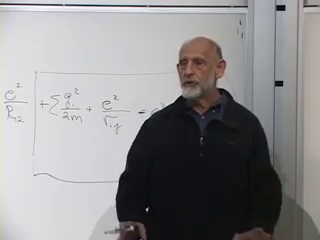
\includegraphics[width=0.72\textwidth]{lecture_01_figure_02.png}
\caption{介紹電子基態問題時，分子哈密頓量仍留在黑板上。式~\eqref{eq:molecular-hamiltonian}的排版形式列出了畫面中被遮住的各項。}
\lectureframe{00:16:19}
\end{figure}

\begin{classroomqa}
\audiencequestion{原子核的動量只是被設為零嗎？\lecturetimestamp{00:15:39}}
\lecturerresponse{只是暫時如此。在最低階近似中，原子核被視為固定不動，因為它們的運動遠比電子慢。求解有效的原子核問題時，我們會把原子核的動量納入，因此這項近似並未違反不確定性原理。}
\end{classroomqa}

電子基態能量現在成為原子核所感受到的有效位能的一部分：
\begin{equation}
V_{\mathrm{eff}}(R_1,R_2)
=\frac{e^2}{R_{12}}+E_{\mathrm{el}}(R_1,R_2).
\label{eq:molecular-effective-potential}
\end{equation}
對兩個孤立原子而言，轉動和平移不變性使這個位能只依賴兩原子間距 \(R_{12}\)。在距離極短時，原子核之間的庫侖排斥占主導；距離極遠時，交互作用很弱。在這兩個極限之間，電子雲可以形成吸引區域和一個極小值。原子核的波函數因而集中在該極小值附近，描述出一個束縛分子。

請注意運算順序。我們並不是猜出一個經驗上的吸引力就把電子丟開，而是先在固定的原子核背景下求解電子的量子問題，之後才消去電子的顯式座標，保留所得的本徵值。短距離物理的效應保留在 \(V_{\mathrm{eff}}\) 的形狀、深度和曲率之中。極小值的位置決定平衡間距；曲率決定小振動的性質；漸近形式則決定束縛態是否存在。一個有效函數就把所有這些電子資訊帶入較慢的問題。

因此，複雜的多電子哈密頓量已轉化為帶有新位能的雙原子核哈密頓量。我們消去了快速自由度，同時完整保留它們對低能物理的影響。這個位能經過了重整化。熟悉的 Born--Oppenheimer 推理通常不以重整化之名介紹，卻恰好包含我們需要的概念：
\begin{equation}
\begin{gathered}
\text{fast microscopic dynamics}\\
\Downarrow\\
\text{effective parameters for slow dynamics}
\end{gathered}
\end{equation}

\section{自然單位制與場的量綱}

在量子場論中，要消去的模式也可以稱為短距離、短波長、高頻率或高能量模式。在畫費曼圖之前，先確定量綱的計算方式。

一般力學使用彼此獨立的長度、時間和質量單位。在粒子物理中，我們令
\begin{equation}
\hbar=c=1.
\end{equation}
如此一來，能量和質量由 \(E=mc^2\) 聯繫起來；由於 \(c=1\)，長度和時間等價；而 \(\hbar=1\) 使動量成為長度的倒數。最後只剩下一種量綱：
\begin{equation}
[M]=[E]=[p]=L^{-1},
\qquad
[x]=[t]=L.
\label{eq:natural-units}
\end{equation}

這並沒有消除量綱，而是選定換算因子，讓時間可以用長度表示，質量可以用長度的倒數表示。只要指定一個單位，其他單位就都隨之確定。因此，截斷尺度既可以用短距離 \(\delta\) 描述，也可以用高能量 \(\Lambda=1/\delta\) 描述：兩者只是同一尺度的不同說法。

考慮一個實標量場 \(\phi\)，其拉格朗日密度採用以下示意性的正規化：
\begin{equation}
\mathcal L=(\partial_\mu\phi)(\partial^\mu\phi)-V(\phi),
\qquad
S=\int d^4x\,\mathcal L.
\label{eq:scalar-action}
\end{equation}

\begin{figure}[htbp]
\centering
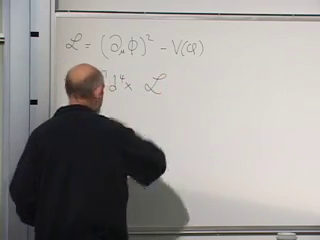
\includegraphics[width=0.78\textwidth]{lecture_01_figure_03.png}
\caption{局域的標量拉格朗日密度，以及將它對時空積分所得的作用量。}
\lectureframe{00:26:08}
\end{figure}

拉格朗日密度是局域的，描述單一時空點。經典場方程由作用量取駐值的條件導出。在量子理論中，同一個作用量出現在路徑積分的相位 \(\exp(iS)\) 中。無論採用哪種觀點，\(S\) 的量綱都至關重要。恢復 \(\hbar\) 後，相位為 \(\exp(iS/\hbar)\)；令 \(\hbar=1\) 後，\(S\) 本身必須是無量綱的。

\begin{classroomqa}
\audiencequestion{作用量的單位是\(\hbar\)嗎？\lecturetimestamp{00:26:13}}
\lecturerresponse{是的。既然 \(\hbar\) 已設為一，作用量在這套單位制中就是無量綱的。四維積分測度的量綱是 \(L^4\)，因此拉格朗日密度的量綱必須是 \(L^{-4}\)。}
\end{classroomqa}

現在由動能項決定場的量綱：
\begin{align}
[S]&=1, & [\mathcal L]&=L^{-4},\\
[\partial_\mu]&=L^{-1}, &
[(\partial\phi)^2]&=L^{-2}[\phi]^2=L^{-4},\nonumber\\
&& [\phi]&=L^{-1}.
\label{eq:scalar-dimension}
\end{align}
這個簡單的計算將決定後續所有圖在紫外區的量綱。

將位能展開為
\begin{equation}
V(\phi)=\frac{m^2}{2}\phi^2+g\phi^3+\lambda\phi^4+\cdots.
\label{eq:scalar-potential}
\end{equation}
每一項的量綱都必須是 \(L^{-4}\)。由於
\([\phi^n]=L^{-n}\)，
\begin{equation}
[m^2]=L^{-2},
\qquad
[g]=L^{-1},
\qquad
[\lambda]=1.
\label{eq:coupling-dimensions}
\end{equation}
四次耦合是無量綱的。這類耦合在重整化中特別重要，因為它們對尺度的依賴性無法單從長度的簡單冪次看出。

\begin{classroomqa}
\audiencequestion{\(g\)的單位是質量嗎？\lecturetimestamp{00:29:52}}
\lecturerresponse{是的。因子 \(\phi^3\) 的量綱是 \(L^{-3}\)，而位能密度的量綱必須是 \(L^{-4}\)。因此 \([g]=L^{-1}\)；在自然單位制中，它的量綱就是質量。}
\end{classroomqa}

\section{頂點與短距離傳播子}

費曼規則由頂點和傳播子構成。\(g\phi^3\)項提供一個三線頂點，其因子正比於 \(g\)；\(\lambda\phi^4\)項提供一個四線頂點，其因子正比於 \(\lambda\)。二次項則提供一個局域的兩點插入。可以把它想成一個粒子進入後被吸收，再重新發射出來；其係數正比於 \(m^2/2\)。本講刻意略去數值正規化、正負號、\(i\) 的因子和對稱因子，因為重點在於找出尺度依賴性，而非計算散射截面。

這些圖有其操作上的詮釋。三點頂點可以吸收兩個量子並發射一個量子，也可以代表三條線的其他交叉相關配置。四點頂點可以描述兩個粒子入射、兩個粒子出射。二次項的交叉符號仍代表合法的兩線頂點，雖然通常會把它併入自由傳播子中。我們把它畫出來，是因為稍後可以藉由比較，辨認出每一種未解析的兩點過程。

傳播子連結兩個時空點。圖中的線並不表示量子粒子沿著經典直線運動，而是代表在 \(x\) 產生場激發，並在 \(y\) 將它移除或探測到的振幅：
\begin{equation}
\Delta(x-y)=\langle0|\phi(y)\phi(x)|0\rangle.
\label{eq:position-propagator}
\end{equation}
從右向左讀這個式子。\(\phi(x)\)作用在真空上，會在 \(x\) 產生一個單粒子成分。\(\phi(y)\)作用在左矢上，則移除 \(y\) 的成分。它們的真空矩陣元是第一個時空點產生粒子、第二個時空點探測粒子的重疊振幅。符號 \(x\) 和 \(y\) 代表完整的四向量，不只是兩個笛卡兒座標。

態不帶物理量綱，而每個場帶有量綱 \(L^{-1}\)。因此
\begin{equation}
[\Delta]=L^{-2}.
\end{equation}
無質量場沒有內在的長度尺度，所以量綱分析決定其短距離行為為
\begin{equation}
\Delta(x-y)\sim\frac{1}{(x-y)^2}.
\label{eq:massless-propagator}
\end{equation}
分母是洛侖茲不變的間隔平方；在奇點處須採用通常的處方。\editorialnote{為了進行冪次計數，將間隔作 Wick 轉動至歐幾里得時空會更方便；此時其大小明確地正比於 \(1/|x-y|^2\)。這不會改變以下分析所用的紫外冪次。}

當 \(y\) 趨近 \(x\) 時，傳播子會發散。這種間隔趨近於零時的傳播奇異性，正是更複雜圖形中紫外發散的來源。

\section{標量質量的重整化}

對標量場而言，動力學參數是 \(m^2\)，這點已可從相對論性的色散關係看出：
\begin{equation}
E=\sqrt{\mathbf p^2+m^2}.
\end{equation}
令 \(\delta\) 為有效描述所能解析的最短距離。若頂點間距小於 \(\delta\)，我們便不加以區分。任何這類未解析過程，只要有一個入射標量和一個出射標量，其可觀測的兩點結構就與質量插入相同，因此必須對有效質量有所貢獻。

可以把加速器想成顯微鏡。若它最精細的解析度是 \(\delta\)，那麼在一處吸收、又在遠小於 \(\delta\) 的距離外發射，便無法和真正的局域事件區分。我們刻意在這個尺度上模糊頂點。重整化的規則，就是把所有這類低於解析度、彼此無法區分的過程，納入相應局域算符的係數。

\subsection{第一個四次作用修正}

從一個 \(\phi^4\) 頂點開始。兩條線是外部粒子；另外兩條線形成短迴圈，在幾乎同一點發射並重新吸收。把重合點的傳播子在截斷距離上平滑化，可得
\begin{equation}
\Delta(0)\ \longrightarrow\ \Delta(\delta)\sim\frac{1}{\delta^2},
\end{equation}
因此
\begin{equation}
\delta m^2_{(1)}\sim\frac{\lambda}{\delta^2}.
\label{eq:one-loop-scalar-mass}
\end{equation}
若 \(m_0^2\) 表示輸入參數，也就是裸參數，則低解析度下的兩點係數示意為
\begin{equation}
\frac{m_{\mathrm{eff}}^2}{2}
\sim
\frac{m_0^2}{2}
+c_1\frac{\lambda}{\delta^2},
\label{eq:first-renormalized-mass}
\end{equation}
其中 \(c_1\) 包含此處略去的數值因子和依賴慣例的因子。在無法解析小於 \(\delta\) 距離的實驗中，所測得的實驗室質量就是這個重整化後的量，而非單獨的 \(m_0\)。

因此，觀測到的兩點事件有兩種無法區分的發生方式：原有的二次頂點吸收並重新發射粒子，或者四次交互作用在短暫發射並重新吸收一個虛標量粒子的同時，造成相同結果。量子力學會將振幅相加。當迴圈的尺度低於解析度時，它獨立的歷程不再出現在有效描述中，但它對測得係數的貢獻仍然存在。

\subsection{下一個四次作用修正}

現在把兩個四次頂點連接起來：一個外部粒子從 \(x\) 入射，另一個從 \(x+\Delta\) 出射，兩個頂點之間由三個內部傳播子連接。這裡有兩個 \(\lambda\) 因子，而傳播子則給出 \(\Delta^{-6}\)。量子振幅必須對所有無法解析的出射位置加總，因此要對相對四向量積分：
\begin{equation}
\delta m^2_{(2)}
\sim
\lambda^2
\int_{|\Delta|\gtrsim\delta}
d^4\Delta\,\frac{1}{|\Delta|^6}.
\label{eq:two-loop-power-count}
\end{equation}

\begin{classroomqa}
\audiencequestion{頂點旁的小標記表示那裡只有三個粒子嗎？\lecturetimestamp{00:46:35}}
\lecturerresponse{不是。我們用的仍是四次交互作用，每個頂點都有四條線相接。在這個兩點圖中，一條是外線，另外三條在兩個頂點之間延伸。第二個頂點也同樣有四條線相接。}
\end{classroomqa}

積分測度貢獻長度的四次方，而三個傳播子合計貢獻長度的負六次方。由於紫外截斷是估算中唯一的尺度，
\begin{equation}
\int_{|\Delta|\gtrsim\delta}
\frac{d^4\Delta}{|\Delta|^6}
\sim\frac{1}{\delta^2},
\qquad
\delta m^2_{(2)}
\sim\frac{\lambda^2}{\delta^2}.
\label{eq:two-loop-scalar-mass}
\end{equation}
這裡的 \(\Delta^\mu\) 是四分量積分變數；積分涵蓋時間分量和三個空間分量。小寫的 \(\delta\) 則是固定的截斷距離。講課時一開始對兩者使用相同的口頭稱呼，之後才更正記號。

把四維測度改寫成徑向形式，也能看出相同結果。略去角度積分所給的常數，
\begin{equation}
\int_{\delta}\frac{d^4\Delta}{|\Delta|^6}
\sim
\int_{\delta}\frac{R^3\,dR}{R^6}
=\int_{\delta}\frac{dR}{R^3}
\sim\frac{1}{\delta^2}.
\end{equation}
因此，大距離端的積分上限對紫外估算並不重要：積分主要由下限決定。

更高階的圖也遵循相同模式。包含更多四次頂點的圖會帶來更高次的 \(\lambda\)，但量綱分析仍允許質量修正呈二次發散：
\begin{equation}
\begin{aligned}
m_{\mathrm{eff}}^2
={}&m_0^2
+\frac{1}{\delta^2}
\left(c_1\lambda+c_2\lambda^2+c_3\lambda^3+\cdots\right)\\
&+\text{weaker terms}.
\end{aligned}
\label{eq:scalar-mass-series}
\end{equation}

\subsection{三次交互作用與對數發散}

兩個三次頂點之間有兩個傳播子，連接鄰近的時空點。其貢獻的尺度關係為
\begin{equation}
\delta m_g^2
\sim
g^2\int_{|\Delta|\gtrsim\delta}
\frac{d^4\Delta}{|\Delta|^4}.
\label{eq:cubic-loop}
\end{equation}
此時測度和分母帶有相同的冪次，因此剩下的是對數依賴，而非冪次依賴：
\begin{equation}
\delta m_g^2
\sim
c_g g^2\log\!\left(\frac{1}{\mu\delta}\right).
\label{eq:cubic-log}
\end{equation}
參考尺度 \(\mu\) 使對數的引數成為無量綱量。這就是講課中示意寫法 \(g^2\log\delta\) 的完整量綱形式。對數的變化遠比任何逆冪緩慢，因此截斷距離縮短時，\(1/\delta^2\) 會占主導。

徑向形式再次清楚呈現這項差異：
\begin{equation}
\int_{\delta}^{R_{\mathrm{IR}}}
\frac{d^4\Delta}{|\Delta|^4}
\sim
\int_{\delta}^{R_{\mathrm{IR}}}\frac{R^3\,dR}{R^4}
=\log\!\left(\frac{R_{\mathrm{IR}}}{\delta}\right).
\end{equation}
測度和分母的冪次相同時會產生對數；分母的冪次較高時，則產生截斷距離的逆冪。這裡不需要計算角度因子；講課的目的，是教我們一眼看出紫外行為。

\begin{classroomqa}
\audiencequestion{這裡的對數是以什麼為底？\lecturetimestamp{00:57:42}}
\lecturerresponse{使用自然對數。改變底數只會乘上一個數值常數，而這個常數會併入係數中。此處尚未計算該係數內的 \(2\)、\(\pi\) 和對稱因子。}
\end{classroomqa}

\begin{classroomqa}
\audiencequestion{對長度取對數，量綱上不會出問題嗎？質量修正的量綱又從何而來？\lecturetimestamp{00:58:32}}
\lecturerresponse{對數比較的總是兩個尺度；嚴格來說，取對數的必須是 \(1/(\mu\delta)\) 這類無量綱比值。耦合 \(g\) 的量綱是質量的一次方，因此 \(g^2\) 的量綱恰好是質量平方，符合修正項所需的量綱。}
\end{classroomqa}

\begin{classroomqa}
\audiencequestion{費曼圖給出振幅。振幅的絕對值平方就是機率嗎？\lecturetimestamp{00:59:41}}
\lecturerresponse{若把振幅放進實際的躍遷計算，並納入所需的態因子和相空間因子，是的。這裡更直接的用途則不同：未解析的兩點振幅具有與質量項相同的局域形式，因此會改變有效質量參數。}
\end{classroomqa}

\section{所有參數都會成為有效參數}

質量修正圖形有無窮多個，並不會因為 \(\lambda\) 很小就消失。微擾論依耦合常數的冪次排列這些圖，因此後續各項可能逐次變小，但圖形仍有無窮多個。同樣的短距離消去也會使交互作用本身受到重整化。

\begin{classroomqa}
\audiencequestion{即使是質量重整化，也有無窮多個圖形嗎？\lecturetimestamp{01:00:35}}
\lecturerresponse{沒錯。如果 \(\lambda\) 足夠小，微擾級數可能仍然有用，因為高次項會逐次受到抑制。不過，重整化後的參數由整個級數定義，而不只由第一個圖形決定。}
\end{classroomqa}

從操作上來說，局域的 \(\lambda\phi^4\) 交互作用就是一個兩粒子入射、兩粒子出射的振幅。若更複雜的四點過程完全發生在無法解析的區域內，在低解析度下便無法和原來的局域頂點區分。因此，這些圖形都併入有效的 \(\lambda\)。在四維 \(\phi^4\) 理論中，它們的主導尺度依賴通常呈對數形式。本講並未計算該貝他函數，而是以此例說明一項普遍原則：
\begin{equation}
\begin{gathered}
\text{parameters measured at low energy}\\
\ne\\
\text{parameters entered at the microscopic cutoff}
\end{gathered}
\end{equation}

四點例子很重要，因為它排除了可能的誤解：重整化不是只用來處理質量發散的特殊修補。拉格朗日量中每個允許的算符，都可以由具有相同外部線和對稱性的未解析圖形再現。兩點過程會重整化二次項係數，四點過程會重整化四次項係數，而真空到真空的過程則會重整化常數項。低能拉格朗日量是一份精簡的帳目，記錄了所有這些短距離過程。

\begin{classroomqa}
\audiencequestion{既然 \(\Delta\) 的量綱是長度，對它取對數在量綱上不會有問題嗎？另外，黑板上的大寫和小寫 delta 是否曾經對調？\lecturetimestamp{01:01:34}}
\lecturerresponse{這裡的對數實際上是尺度之比，因此是無量綱的。沒錯，記號一度對調：\(\Delta^\mu\) 是積分變數，而 \(\delta\) 是最後留在答案中的最小距離截斷。}
\end{classroomqa}

這是分子範例在場論中的對應情況。我們解出不可見的快速電子所產生的效應，並將結果納入位能。此處則是加總不可見的短距離過程，再將結果納入質量、耦合常數和其他所有允許的局域係數中。所有參數都會改變。

\begin{classroomqa}
\audiencequestion{可以再說明一次嗎？測得的量是否包含實驗看不到的更小尺度所產生的效應？\lecturetimestamp{01:05:13}}
\lecturerresponse{是的。這些尺度上的個別漲落無法解析，但加總後的效應仍然存在。所有涉及更短尺度的圖形都會合併到單一有效係數中；低能實驗稱這個係數為物理質量平方等參數。}
\end{classroomqa}

\begin{classroomqa}
\audiencequestion{那輸入項 \(m_0^2\) 是否必須抵消其他貢獻？\lecturetimestamp{01:06:00}}
\lecturerresponse{如果測得的標量質量遠小於各個紫外貢獻，就必須如此。這種所需的抵消，就是接下來要談的精細調節問題。}
\end{classroomqa}

\section{希格斯層級問題}

假設截斷距離就是普朗克長度，那麼有效場論就得概括從實驗室尺度到量子重力必須介入之尺度間的漲落。
以粒子物理單位表示，
\begin{equation}
\delta\sim M_{\mathrm{Pl}}^{-1}\sim10^{-19}\,\mathrm{GeV}^{-1},
\qquad
\frac{1}{\delta^2}\sim10^{38}\,\mathrm{GeV}^2.
\label{eq:planck-cutoff}
\end{equation}
採用約化或未約化的普朗克尺度，並不影響這項巨大尺度差異的比較。

長度尺度之間的差異同樣驚人。普朗克長度比質子半徑小約十九個數量級，比本講所討論的加速器直接探測距離小約十六或十七個數量級。將這段長度差平方，就得到標量質量平方參數中約三十四位數的抵消。

希格斯場是標量場；所需的弱尺度約為數百 GeV，而不是 \(10^{19}\) GeV。然而，式~\eqref{eq:scalar-mass-series}中的各項自然可以達到普朗克尺度。這些項的正負號尚未逐一確定：有些可能為正，有些可能為負，裸質量平方也可能為正或負。但若要留下電弱尺度的結果，這些巨大項目就必須在約三十四位小數的精度內彼此抵消。Susskind 起初說十七位，隨後便更正，因為這裡比較的是質量平方。這種微調程度由質量平方之比決定。

\begin{classroomqa}
\audiencequestion{\(\lambda\)是小於還是大於 1？\lecturetimestamp{01:09:50}}
\lecturerresponse{假設它略小於 1。若逐次冪愈來愈大，微擾理論就會變得難以處理；而純標量理論在四次耦合任意大的情況下，也無法一致地外推。不過，\(\lambda\)遠沒有\(10^{-38}\)那麼小；講座以百分比量級的數值作為參考。}
\end{classroomqa}

\begin{classroomqa}
\audiencequestion{即使\(\lambda<1\)，是不是仍有許多項因為各自都帶有很大的截斷因子而舉足輕重？\lecturetimestamp{01:10:43}}
\lecturerresponse{是的。更高次冪最終會抑制級數，但在抑制作用顯現之前，仍可能有許多項作出貢獻。這些項和裸項都必須彼此精確配合，才能留下極其微小的物理結果。}
\end{classroomqa}

回顧一下為什麼希格斯質量參數已知處於弱尺度。依照講座採用的慣例，將對稱破缺勢寫成
\begin{equation}
V(\phi)=-\frac{\mu^2}{2}\phi^2+\frac{\lambda}{4}\phi^4.
\label{eq:higgs-potential}
\end{equation}
負的二次項係數使原點不穩定，正的四次項則使勢能保持穩定。對勢能微分，
\begin{equation}
\frac{dV}{d\phi}=-\mu^2\phi+\lambda\phi^3
=\phi(-\mu^2+\lambda\phi^2),
\end{equation}
可得非零極小值
\begin{equation}
\phi_{\min}^2=f^2=\frac{\mu^2}{\lambda}.
\label{eq:higgs-minimum}
\end{equation}
黑板上將四次項概略寫成\(\lambda\phi^4\)，但引用的是式~\eqref{eq:higgs-minimum}；補上慣用因子\(1/4\)後，這兩處便一致，而論證本身不變。

\(-\mu^2\)的符號很重要，但無法解決自然性問題。驅動自發對稱破缺的是原點處的負曲率。重整化會以很大的正、負貢獻改變這個曲率。觀測到的破缺真空要求這些貢獻的總和不只要很小，還必須恰好是特定的小負值，才能使極小值落在弱尺度。

\(W\)與\(Z\)玻色子的質量，決定了\(f\)在講座採用的粗略歸一化下約為\(200\,\mathrm{GeV}\)。若\(\lambda\)既不極大也不小得驚人，\(\mu\)就必須大致處於相同量級。因此，觀測到的弱尺度係數，是若干個各自可能大上數十個數量級的貢獻相加後所剩下的結果。

這個問題稱為希格斯微調問題、階層問題或規範階層問題。所謂階層，指的是一般弱尺度與可能的大統一尺度或普朗克尺度之間的巨大比值。數值很小本身未必構成悖論；真正令人不安的是，這個小數值由幾個很大、看似互不相關的部分組成，而它們必須以極高精度相消。這個問題在1970年代末、1980年代初便已受到重視；尋找這種相消背後的機制，促使人們提出超對稱以及其他幾種競爭性的構想。

無限微擾級數使這個謎題更加尖銳，而非將它消除。百分比量級的\(\lambda\)會使足夠高次的冪變小，但在抑制作用佔上風之前，仍可能有許多項作出貢獻。只靠單圈貢獻偶然抵消裸質量並不足夠；納入其餘短距離過程後，有效弱尺度仍必須保持穩定。若各項之間存在結構性的關係，便能構成解釋；若只是彼此無關的數字逐位相消，那就只是微調。

\section{為什麼費米子質量的情況較好}

標準模型的其他粒子不需要承受同類的獨立微調。狄拉克費米子的質量項為
\begin{equation}
\mathcal L_m=-m\bar\psi\psi
=-m\left(\bar\psi_L\psi_R+\bar\psi_R\psi_L\right).
\label{eq:fermion-mass}
\end{equation}
這個質量項含有質量，而非質量的平方，並且耦合左右手徵態。因此，局域的質量插入會將\(L\)轉變為\(R\)，或將\(R\)轉變為\(L\)。

\begin{figure}[htbp]
\centering
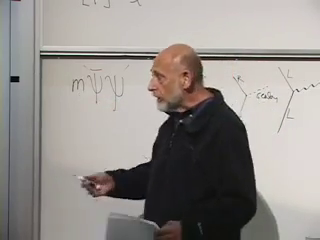
\includegraphics[width=0.76\textwidth]{lecture_01_figure_04.png}
\caption{費米子質量項，以及黑板上改變手徵性的線條示意圖。由於部分粉筆筆跡被遮住，以下會根據代數關係重建這些圖。}
\lectureframe{01:23:36}
\end{figure}

講課時常會說手性或螺旋度。若要精確描述這種保護機制，以手徵性表述最為清楚。對於超相對論性粒子，螺旋度的圖像可以提供直觀理解；不過，式~\eqref{eq:fermion-mass}中的左右手場所帶有的量是手徵性。

規範相互作用會保持手徵性：
\begin{equation}
L\xrightarrow{\ \gamma\ }L,
\qquad
R\xrightarrow{\ \gamma\ }R.
\label{eq:gauge-preserves-chirality}
\end{equation}
與標量場的湯川相互作用則會連結相反的手徵性：
\begin{equation}
L\xleftrightarrow{\ \phi\ }R.
\label{eq:scalar-flips-chirality}
\end{equation}
先假設電子以\(m_0=0\)開始。無論發射並重新吸收多少光子，都無法產生質量，因為每個規範頂點都保持手徵性。從左手開始的整個過程便會一直保持左手。因此，純量子電動力學可以一致地容許無質量電子：電磁自能無法在質量為零時產生額外的質量。

在線條圖像中，先從左手徵電子開始。經過第一個光子頂點後，它仍是左手徵；光子傳播並被重新吸收後，它依然是左手徵。重複這個過程只會加入更多保持手徵性的頂點。外部二點函數可以經過重整化，但不會因此產生定義質量所需的左右手結構。

發射標量粒子能做到嗎？一個標量頂點會將\(L\)轉變為\(R\)，但發射出的標量粒子必須再被吸收。因此，二點自能圖中會有偶數個標量頂點。第二次翻轉會抵銷第一次，所以完整的圖仍保持外部手徵性。無論內部圖有多複雜，發射與重新吸收都會使頂點成對出現，因而在起始質量為零時，無法產生可加的\(L\)到\(R\)項。

這是根據翻轉次數奇偶性所作的論證。一個標量頂點會使手徵性翻轉一次；每條內部標量線都必須閉合，因此需要另一個端點，也就需要第二次翻轉。四個標量頂點會造成四次翻轉，依此類推。翻轉偶數次後，費米子會回到原本的手徵性。這個結論不限於黑板上畫出的最簡單圈圖。

只有在圖中已經有質量插入時，才可能產生非零的質量修正。例如，光子的發射與重新吸收可以發生在一個\(m_0\bar\psi\psi\)插入的兩側。規範頂點帶來電荷的二次方，而唯一一次手徵性翻轉則帶入原有的質量：
\begin{equation}
\begin{aligned}
m_e
&=m_0+c_1e^2m_0+c_2e^4m_0+\cdots\\
&=m_0\left(1+c_1e^2+c_2e^4+\cdots\right).
\end{aligned}
\label{eq:multiplicative-fermion-mass}
\end{equation}
若\(m_0=0\)，結果仍為零。若\(m_0\)很小，每一項修正都正比於這個小量。我們仍可以追問，為什麼電子相對於基本尺度如此之輕；但不必再靠相減巨大而互不相關的數值來得到電子質量。就這個意義而言，小的費米子質量在技術上是自然的。

質量插入清楚展現了這個允許的過程。從\(L\)開始。光子發射會保持\(L\)；插入\(m_0\)後，\(L\)轉變為\(R\)；光子重新吸收則保持\(R\)。此時，圖的外部手徵性符合質量項的形式，但其數值必然含有因子\(m_0\)。這正是它與式~\eqref{eq:one-loop-scalar-mass}的關鍵差異：即使將起始標量質量設為零，式中的標量修正仍不為零。

規範玻色子也受到類似的保護：規範對稱性禁止獨立的質量項，因此起初無質量的規範玻色子，在所有微擾階數下都會保持無質量。在標準模型中，費米子和弱規範玻色子的質量來自對希格斯期望值的響應。只要控制好希格斯尺度，其餘輕粒子的質量就不必各自再經歷同樣災難性的微調。

這指出了超對稱意圖處理的問題：理論能否阻止希格斯標量獲得巨大的可加質量修正？在適當的超對稱架構中，答案是肯定的，因為玻色子與費米子的貢獻彼此相關，而非各自獨立。詳細機制將從下一講開始說明。

\section{另一種微調：真空能量}

還有一個更嚴重的重整化問題，但只有納入引力後才會成為可觀測現象。在非引力物理中，對所有能量加上同一個常數，不會改變任何實驗結果。例如，電子質量不是絕對能量，而是從真空中加入一個電子所需的額外能量：
\begin{equation}
m_e=E(\text{vacuum}+\text{one electron})-E(\text{vacuum})
\end{equation}
這是在電子靜止系中定義的。若真空與所有激發態的能量一起平移，它們之間的差值便保持不變。

然而，真空到真空的圖確實會改變真空能量。在\(\lambda\phi^4\)理論中，將一個四次頂點的四條線接成兩個短迴圈。每個重合的傳播子都貢獻\(1/\delta^2\)，因此
\begin{equation}
\delta\rho_{\mathrm{vac}}
\sim
c_{\mathrm{vac}}\frac{\lambda}{\delta^4}.
\label{eq:vacuum-energy-divergence}
\end{equation}
更複雜的真空圖會帶有不同的耦合因子和係數，但量綱分析通常仍會得到相同的四次截斷尺度依賴，出現在能量密度中。

沒有外部線，正是辨認這項修正的關鍵。二點圖比較單粒子態與真空，因而改變質量；四點圖會改變散射；沒有入射或出射粒子的圖，則會改變真空到真空的振幅本身。一個四次頂點帶來\(\lambda\)，它的兩個短迴圈則各帶來\(\delta^{-2}\)。依量綱分析，能量密度便會具有\(\delta^{-4}\)的尺度。

沒有引力時，人們可以任意選定能量的零點，並且認為這不會造成影響。廣義相對論則取消了這項自由：應力能量會產生時空曲率，因此均勻的真空能量也會使空無一物的空間產生引力。真空能量表現為宇宙常數，並在觀測上與暗能量相關。因此，實測到的微小真空能量必須在形如\(\delta^{-4}\)的貢獻之下仍保持微小。

這就是納入引力後，問題為何會改變。在普通量子力學中，將每個能階都平移同一個常數，不會改變躍遷頻率。在引力中，這個常數並非無關緊要：真空的應力張量正比於度規，會使時空彎曲。原本任意選定的能量零點，於是成了愛因斯坦方程中的源。

因此，至少存在兩個極端的自然性難題。講座估計，真空能量的微調約涉及123位小數，希格斯質量的微調則約涉及30--35位。確切數目取決於紫外尺度與採用的慣例，但兩者差異之大毫無疑問。超對稱或許能回應這裡討論的希格斯問題；然而，超對稱一旦破缺，本身並不能解釋觀測到的宇宙常數。\editorialnote{這也說明了為什麼精確超對稱下玻色子--費米子的相消，無法在現象學上解決觀測到的真空能量問題：我們的世界中超對稱必須破缺。}

\section{課堂提問總結}

\begin{classroomqa}
\audiencequestion{希格斯修正取決於截斷尺度\(\delta\)，但截斷尺度似乎是任意的。它可以是普朗克長度、普朗克長度的十倍，或是別的尺度嗎？這是否代表微調也是任意的？\lecturetimestamp{01:33:50}}
\lecturerresponse{數值貢獻取決於有效理論所適用的最短尺度。這種依賴是物理計算的一部分，不能藉此迴避問題。只要標準模型在某個尺度上仍然適用，該尺度的模式及其效應就必須納入計算。可以選擇在預期新物理出現的距離處設定\(\delta\)---，例如普朗克尺度，或接近\(10^{16}\,\mathrm{GeV}\)的大統一尺度。累積到該尺度的貢獻，已經構成這個問題的一個下限。若將同一理論延伸至更短距離，二次敏感性只會更大。我們必須解釋，從實驗室尺度到那個紫外邊界之間，各個尺度的貢獻是如何被抵消的。}
\end{classroomqa}

\begin{classroomqa}
\audiencequestion{如何定義標量粒子？有什麼例子？\lecturetimestamp{01:37:26}}
\lecturerresponse{希格斯粒子就是這裡要舉的例子。標量在空間旋轉下不會轉變成不同的分量；換言之，它的粒子量子自旋為零。光子以向量場描述，引力場則以張量描述。在2010這場講座進行時，還沒有探測到任何基本的零自旋粒子。\editorialnote{希格斯玻色子於2012年在 CERN 被發現，其測量性質與零自旋相符。}}
\end{classroomqa}

\begin{classroomqa}
\audiencequestion{\(Z\)粒子也是規範玻色子嗎？\lecturetimestamp{01:38:31}}
\lecturerresponse{是。\(Z\)、\(W^+\)和\(W^-\)都是自旋為 1 的規範玻色子，光子也是如此。它們的場方程與相互作用，是麥克斯威式規範描述在非阿貝爾或電弱理論中的推廣。}
\end{classroomqa}

\begin{classroomqa}
\audiencequestion{為什麼玻色子的基態貢獻不會抵消真空能量中的費米子貢獻？\lecturetimestamp{01:39:10}}
\lecturerresponse{費米子迴圈與相應的玻色子迴圈，確實可能以相反符號出現。但抵消並非自動發生：粒子的質量、多重度和耦合都必須匹配。即使只有些微差異，也會留下對截斷尺度敏感的巨大殘值；而無窮多族的圖也必須逐階匹配。精確超對稱會強制玻色子--費米子之間存在這類關係。一般的非超對稱粒子內容則不會如此；超對稱破缺後，真空能量問題仍會留下。}
\end{classroomqa}

\section{展望}

本講的安排有其用意。首先，分子計算說明消去快變數既不是忽略它們，也不是變魔術：快變數的基態能量會成為慢變數的勢能。量子場論則在不同波長上重複這項操作。接著，量綱分析揭示哪些有效參數會對截斷尺度敏感。標量質量會得到正比於\(\delta^{-2}\)的加性項，因此小的希格斯尺度顯得異常脆弱。手徵性保護零質量極限，使費米子質量接受乘性重整化；規範對稱性也同樣保護無質量規範玻色子。真空能量的敏感性更高，按\(\delta^{-4}\)的尺度變化；引力則使它的絕對值成為可觀測量。

超對稱正是在這個時刻進入課程：它不是裝飾性的新數學，而是試圖讓標量部門的表現更接近受到保護的部門。接下來要理解的是，什麼樣的對稱性可以將玻色子和費米子緊密聯繫起來，並藉此組織這些相消。
\chapter{費米子符號與超對稱相消}

\lectureoverview{超對稱將玻色子與費米子聯繫起來，但在寫下其代數之前，先看看為何需要這種關係會更容易理解。我們先從旋轉的拓撲談起，接著透過干涉讓費米子波函數的符號成為可觀測量，再由交換反對稱性推導閉合費米子圈的負號，最後運用玻色子圈與費米子圈符號相反這一點，說明真空能與標量自能為何可能相消。後半部則探討超對稱可以破缺到什麼程度、如何探測超對稱伴粒子，以及為什麼精確超對稱會抹去一般原子的殼層結構。}

\section{超對稱之前：旋轉的一個奇特之處}

超對稱是費米子與玻色子之間的對稱性。然而，在嘗試構造這種對稱性之前，不妨先回想這兩類粒子對旋轉的反應有多麼不同。這個問題始於一個拓撲事實：它很容易演示，但看過之後卻令人難以忘懷。

手掌朝上，轉動手腕\(2\pi\)。手回到原來的朝向，但手臂顯然沒有回到等價的狀態：它扭轉了。再轉\(2\pi\)，必要時讓手臂跟著移動，就能解開扭轉。因此，在周圍環境保持固定時，\(2\pi\)旋轉無法連續形變至無旋轉，而\(4\pi\)旋轉則可以。這個手部演示，字面上說，就是一種「揮手證明」。

不借助人體解剖也能說明同一件事。把一顆球放在固定的盒子裡，用任意多條柔軟、可伸展但不會斷裂的繩子，將球連接到盒壁。讓球旋轉一周，轉過\(2\pi\)。繩子會糾纏起來，單靠移動繩子無法恢復原來的狀態。若球總共轉過\(4\pi\)，就能讓繩子繞著球移動，直到糾纏解開。盒壁代表空間無窮遠；這個比較之所以有意義，是因為邊界沒有跟著球一起旋轉。

\begin{classroomqa}
\audiencequestion{能不能轉動盒子來解開繩子的糾纏？\lecturetimestamp{00:02:53}}
\lecturerresponse{那就改變了問題。盒子代表空間無窮遠，因此保持固定。我們比較的是物體相對於周圍環境的旋轉，而不是物體與環境一起旋轉。}
\end{classroomqa}

\begin{classroomqa}
\audiencequestion{為什麼不把球再轉\(2\pi\)？\lecturetimestamp{00:03:20}}
\lecturerresponse{這正是兩種情形的差別。若不再繼續轉動球，一次\(2\pi\)旋轉留下的糾纏就無法解開。再轉一周，總共轉過\(4\pi\)之後，糾纏便能解開。}
\end{classroomqa}

用現代群論的語言來說，旋轉群的閉合路徑有兩種拓撲類別：
\begin{equation}
\pi_1\!\left(SO(3)\right)\cong \mathbb Z_2.
\end{equation}
遍歷一次屬於非平凡類別，遍歷兩次則屬於平凡類別。
換句話說，\(SU(2)\)是\(SO(3)\)的雙重覆蓋。這便是費米子符號的幾何前史。

\editorialnote{\(SO(3)\)、\(SU(2)\)與基本群等數學語言，讓拓撲結構一目了然。手臂和繩子的演示則從幾何上呈現了同樣的二值性。}

\section{\texorpdfstring{\(2\pi\)}{2 pi}旋轉對量子態的作用}

現在固定粒子的位置，只考慮它的自旋態，記為\(\ket{\psi}\)。整數自旋粒子是玻色子，半整數自旋粒子是費米子。要實現物理旋轉，可以將帶電自旋置於強磁場中並轉動磁場，也可以讓自旋在固定磁場中進動所需的角度。

\begin{classroomqa}
\audiencequestion{在實驗室裡，究竟要如何旋轉電子自旋？\lecturetimestamp{00:05:26}}
\lecturerresponse{磁場提供了操控自旋的方式。可以轉動足夠強的磁場，讓自旋跟著磁場轉動；也可以讓自旋繞著固定磁場進動。徒手抓住電子並不是可行的實驗方法。}
\end{classroomqa}

假設完整旋轉\(2\pi\)會使量子態乘上一個相位：
\begin{equation}
R(2\pi)\ket{\psi}=\xi\ket{\psi}.
\end{equation}
將此操作執行兩次，得到
\begin{equation}
R(4\pi)\ket{\psi}=\xi^2\ket{\psi}.
\end{equation}
由於\(4\pi\)路徑在拓撲上屬於平凡類別，在這裡的比較中，它必須等同於恆等操作。因此
\begin{equation}
\xi^2=1,
\qquad
\xi=+1\ \hbox{or}\ -1.
\end{equation}
玻色子對應正號，費米子對應負號：
\begin{align}
R(2\pi)\ket{\psi_B}&=+\ket{\psi_B},\\
R(2\pi)\ket{\psi_F}&=-\ket{\psi_F}.
\end{align}
對於自旋確定為\(j\)的態，可以簡潔地寫成
\begin{equation}
R(2\pi)=(-1)^{2j}.
\end{equation}
逐字稿簡短地說，第二種可能是乘以\(2\pi\)；但從前後推導及板書論證可知，原意應是乘以\(-1\)。

乍看之下，這似乎沒有物理意義。若整個波函數變號，
\begin{equation}
\Psi\longmapsto-\Psi,
\end{equation}
機率仍然不變，因為
\begin{equation}
(-\Psi)^*(-\Psi)=\Psi^*\Psi.
\end{equation}
準備兩組狀態相同的電子，將其中一組的每個電子旋轉\(2\pi\)，另一組則保持不動。對任何單獨電子進行測量，都無法判斷它來自哪一組。整體相位不是可觀測量。

\section{讓負號成為相對量}

若只對波函數的一個相干分支施加符號變化，而不影響另一分支，這個符號就能被觀測到。讓電子逐一通過雙路徑裝置。不要測定電子走哪條路徑，因為路徑資訊會破壞干涉。令上、下兩條路徑的振幅分別為\(\psi_1\)與\(\psi_2\)，重新合併後的態就是
\begin{equation}
\Psi=\psi_1+\psi_2.
\end{equation}
設想暫時將兩個分支各自限制在一個磁場區域內。只將第二個分支所經區域的磁場旋轉\(2\pi\)。若粒子是費米子，態便變為
\begin{equation}
\Psi'=\psi_1-\psi_2.
\end{equation}
這就不再是整體符號變化。相對相位會使干涉極大值與極小值互換。若返回的兩個波包以探測器中央為對稱中心、互為鏡像，反對稱組合在中央便會相消為零：
\begin{equation}
\Psi'(0)=\psi_1(0)-\psi_2(0)=0.
\end{equation}
因此，在這個對稱點絕不會探測到電子。若改為同時旋轉兩個分支，則會得到\(-\psi_1-\psi_2=-\Psi\)，不會產生可觀測效應。

講座強調這項實驗的關係性。讓一個磁場區域相對於另一個區域旋轉，就像球旋轉而盒子保持固定；讓兩個區域一起旋轉，則像球和盒子一起轉動。相對旋轉\(4\pi\)會使效應消失，因為此時費米子態回到原狀時帶有正號。這項實驗由 Yakir Aharonov 與 Leonard Susskind 於1967年提出，講座也順帶提到，它後來以干涉儀實現。同一原理也適用於電子或帶電離子：若干涉條紋移動，表示自旋為半整數；若條紋不移動，則表示自旋為整數。

\begin{classroomqa}
\audiencequestion{若相對磁場轉過\(4\pi\)，移動後的條紋會回到原來的位置嗎？\lecturetimestamp{00:12:21}}
\lecturerresponse{會。兩次符號變化相乘得到\(+1\)，造成極大值與極小值互換的相對相位便消失了。}
\end{classroomqa}

\begin{classroomqa}
\audiencequestion{盒子裡的繩子應該在多大程度上被視為與費米子有字面上的關聯？\lecturetimestamp{00:13:43}}
\lecturerresponse{那些繩子是用來記憶拓撲的比喻，並非真的繫在電子上的物理繩子。玻色子的行為就像轉過\(2\pi\)後不留任何痕跡；費米子則恰好保留了非平凡糾纏所代表的符號痕跡。}
\end{classroomqa}

\begin{classroomqa}
\audiencequestion{兩個磁場區域裡各有一個電子嗎？一個被旋轉，另一個沒有？\lecturetimestamp{00:14:29}}
\lecturerresponse{不是。只有一個電子，處於相干的空間疊加態。它有振幅分布在兩個分支上，而裝置不能揭露它位於哪個分支。旋轉一個區域會改變一個振幅相對於另一個振幅的相位；同時旋轉兩個區域則只會改變共同相位。}
\end{classroomqa}

角度\(2\pi\)很特殊，因為自旋方向會回到原狀，而旋量會多出一個負號。一般的相對旋轉也會改變自旋方向。若兩條路徑的自旋態分別以\(\ket{\chi_1}\)和\(\ket{\chi_2}\)返回，干涉項便正比於
\begin{equation}
\braket{\chi_1}{\chi_2}.
\end{equation}
其大小決定條紋的可見度。\editorialnote{自旋重疊公式是對講座中干涉部分減弱或完全消失之定性討論的標準補充。}若自旋態彼此正交，就能完整判定粒子走過哪條路徑，因此不會發生干涉。

\begin{classroomqa}
\audiencequestion{如果測量電子位於哪個磁場區域，會發生什麼事？\lecturetimestamp{00:18:03}}
\lecturerresponse{干涉圖樣會消失。任何能分辨兩條路徑的紀錄，都會破壞兩個振幅的相干疊加。}
\end{classroomqa}

\begin{classroomqa}
\audiencequestion{如果所有自旋一開始都朝同一方向，最後再測量自旋，\(2\pi\)這項操作本身會改變那個方向嗎？\lecturetimestamp{00:18:17}}
\lecturerresponse{不會。經過\(2\pi\)旋轉後，物理上的自旋方向仍與原來相同；只有費米子分支多了一個負號。正因如此，這項操作可以改變干涉，卻不會留下不同的自旋方向作為路徑標記。}
\end{classroomqa}

\begin{classroomqa}
\audiencequestion{如果磁場只轉過\(\pi\)，而不是\(2\pi\)，會怎麼樣？\lecturetimestamp{00:18:43}}
\lecturerresponse{那麼自旋方向就會改變。上自旋分支與下自旋分支可以彼此區分，因此無法干涉。中間角度會使可見度逐漸降低；相對旋轉\(180^\circ\)則會使干涉完全消失。}
\end{classroomqa}

\section{交換對稱性與閉合圈的符號}

旋轉的討論已經揭示一個費米子負號。全同粒子交換時，還會出現另一個密切相關的符號。對於雙粒子波函數，
\begin{align}
P_{12}\Psi_B(1,2)&=+\Psi_B(1,2)=+\Psi_B(2,1),\\
P_{12}\Psi_F(1,2)&=-\Psi_F(1,2)=-\Psi_F(2,1).
\end{align}
玻色子態具有對稱性，費米子態則具有反對稱性。

\begin{figure}[htbp]
\centering
\includegraphics[width=0.74\textwidth]{lecture_02_figure_02.png}
\lectureframe{00:24:27}
\caption{以態記號表示的交換論證。畫面中只有 ket 標記能確實辨認；反對稱性方程式是排印於正文中，並未聲稱是被遮擋的板書內容。}
\end{figure}

現在不必計算積分，就能判定閉合粒子圈的相對符號。考慮一個沒有外腿的真空費曼圖。可以把它想成粒子在時空中走過一條閉合路徑，也可以想成一對粒子與反粒子產生後又湮滅。這種真空圖會貢獻於真空振幅，因而也貢獻於真空能。

先考慮兩個互不連通的圈。不連通圖的貢獻相乘；因此，若單一圈的符號為\(\sigma\)，兩個圈的符號便是
\begin{equation}
\sigma^2=+1.
\end{equation}
在同一時刻，例如\(t=0\)，將兩個圈都切開。這個時間切片上有兩個全同粒子。不交換粒子便重新接合，會恢復成兩個分離的圈；若在接合前交換兩個粒子，拓撲便變成單一的圈。交換對玻色子貢獻\(+1\)，對費米子則貢獻\(-1\)。由於起初兩個圈的符號乘積為正，最後單一圈的符號就是
\begin{equation}
\begin{aligned}
\operatorname{sign}(\text{closed boson loop})&=+1,\\
\operatorname{sign}(\text{closed fermion loop})&=-1.
\end{aligned}
\end{equation}
更一般地，含有\(L_F\)個獨立閉合費米子圈的圖，會帶有因子
\begin{equation}
(-1)^{L_F}.
\end{equation}
講座刻意從粒子交換推導這條規則，而不訴諸格拉斯曼積分。這個初等論證清楚呈現了符號的物理起源。

\section{相反的圈符號與真空能}

玻色子真空圈以一種符號增加真空能的貢獻，費米子圈則以相反符號貢獻。這立刻帶來啟發：觀測到的暗能量密度，與量子場論中粗略的截斷估算相比，極其微小。講座引用的這項著名差異約為\(123\)個數量級。確切的指數取決於採用哪個紫外尺度；關鍵在於兩者之間驚人的落差。

圈圖的貢獻不只取決於統計性質，也取決於質量、電荷、多重度與交互作用。然而，若玻色子與費米子在所有相關性質上都相匹配，它們大小相同的貢獻便可能相消：
\begin{equation}
\begin{gathered}
m_B=m_F,\qquad q_B=q_F,\qquad g_B=g_F,\\
\Delta\rho_{\mathrm{vac}}^{(B)}
+\Delta\rho_{\mathrm{vac}}^{(F)}=0.
\end{gathered}
\end{equation}
這個觀察並未解決宇宙學常數問題，只是提供了普通玻色子圈無法提供的東西：符號相反的貢獻。在適當假設下，精確未破缺的全域超對稱理論確實能使真空能精確相消；超對稱破缺後，觀測到的微小非零值仍未獲得解釋。\editorialnote{這項限定說明，講座提出的動機與更棘手的宇宙學常數問題並非一回事。}

已知精確匹配並不符合自然界的情況。假如電子有一個質量和電荷都相同、自旋為零的伴粒子，電子與正電子經由虛光子湮滅時，就能產生一對這種粒子：
\begin{equation}
e^-e^+\longrightarrow\gamma^*
\longrightarrow\widetilde e^-\widetilde e^+.
\end{equation}
帶電標量粒子若與電子質量簡併，就不可能逃過一般的對撞機實驗。因此，玻色子與費米子之間的對應不可能是觀測到的粒子譜所具有的精確對稱性。這是粒子種類之間的對應，不是物理空間中的反射。

\section{更直接的目標：標量自能}

真空能是第一個例子，但講座主要關注的是標量質量的輻射不穩定性。裸質量為零的標量粒子仍可能受到對截斷尺度呈二次敏感的修正。概略而言，
\begin{equation}
\Delta m_H^2\sim \frac{g_B^2}{16\pi^2}\Lambda^2
\end{equation}
這項修正來自玻色子圈。費米子質量受到另一種機制保護：若無質量費米子具有精確的手徵對稱性，輻射修正就不能產生加法質量項。這就是前一講提到的左右手論證。

現在設想一種足夠嚴格的對稱性，能將標量與費米子納入同一多重態，並使兩者的交互作用相匹配。如此一來，費米子圈就會帶有相反的符號：
\begin{equation}
\Delta m_H^2
\sim
\frac{g_B^2-g_F^2}{16\pi^2}\Lambda^2+\cdots .
\end{equation}
若超對稱要求\(g_B=g_F\)且兩者質量相等，二次項便會相消。如此一來，費米子所受到的保護便延伸到了它的玻色子伴粒子。這不只是兩個費曼圖之間的數值巧合；對稱性必須在每一階及所有允許的交互作用中，確保這種相消。

這幅橫跨整塊黑板的比較，呈現了講座如何從個別圈圖轉向傳播粒子的成對圈圖修正。

\begin{figure}[htbp]
\centering
\includegraphics[width=0.79\textwidth]{lecture_02_figure_04.png}
\lectureframe{00:40:23}

\medskip
\begin{tikzpicture}[scale=0.9]
\draw (-4.2,0) circle (0.55);
\draw[dashed] (-2.4,0) circle (0.55);
\draw (0,0) -- (3.7,0);
\fill (1.85,0) circle (0.055);
\draw (1.85,0) -- (1.85,0.25);
\draw[dashed] (1.85,0.85) circle (0.6);
\end{tikzpicture}
\caption{一般粒子圈圖與伴粒子圈圖拓撲結構的整板對照。排印的草圖只保留了畫面中看得見的拓撲差異，沒有標註被遮擋的粒子名稱。}
\end{figure}

課間休息後，講座從所謂的零階圖像重新開始。這不是微擾論中的階數，而是指最粗略但仍有用的描述：
\begin{quote}
每種粒子都有一個統計性質相反的超對稱伴粒子。每個費米子都有一個玻色子伴粒子，每個玻色子也都有一個費米子伴粒子。
\end{quote}
在精確超對稱理論中，伴粒子也會與原粒子質量簡併，也就是兩者質量相等。自然界並非如此。不過，即使質量不完全相等，只要差距不太大，相消仍可能足以避免標量修正暴增。在軟超對稱破缺下，危險的尺度概略上會由超對稱伴粒子的質量劈裂取代：
\begin{equation}
\Delta m_H^2\sim
\frac{g^2}{16\pi^2}\,\Delta m_{\mathrm{SUSY}}^2
\ln\!\frac{\Lambda^2}{\Delta m_{\mathrm{SUSY}}^2}
\end{equation}
其中還有依模型而異的係數。\editorialnote{這個公式表達了講座中的定性說法：質量無法完全匹配時，會留下由質量劈裂控制的殘餘修正。這個公式並非抄自板書。}

\section{超對稱破缺與2010年的實驗賭注}

這場講座於2010年錄製，當時還沒有觀測到任何超對稱伴粒子。直接的推論是：如果這些伴粒子確實存在，它們必定比已知粒子重，也超出先前實驗設備的探測能力。超對稱模型也區分了兩種粒子：一種只有在電弱對稱性破缺後才取得質量；另一種則可具有較大的、在對稱性保持時就存在的質量。講座以此說明，為什麼超對稱粒子譜中可見的那一半可能較輕，未見的那一半則較重；同時也坦承，這樣的安排有些牽強。Susskind 表示自己預期能探測到超對稱伴粒子，但隨即說明，這只是猜測，並非結論。

因此，大型強子對撞機是這場講座展望的核心。當時預期它會搜尋希格斯玻色子與超對稱伴粒子。這些說法必須放在2010年的背景下理解：講座是在希格斯玻色子發現、以及後來的 LHC 搜尋結果出爐之前，說明當時的實驗賭注。

為什麼受自然性考量驅動的超對稱伴粒子不應該落在普朗克尺度？因為那樣就無法完成它被賦予的任務。若玻色子與費米子的質量相差極大，兩者的圈圖積分在較輕粒子的質量以上便不再相消。剩餘的標量修正大致由較重粒子之間的質量劈裂決定，而非由弱尺度決定。即使超對稱存在於任意遙遠的尺度，它仍是數學上的對稱性，但已無法令人信服地解釋希格斯部門為何如此輕。

講座根據當時的預期，推論相關質量劈裂應在數百 GeV 左右，因此落在 LHC 的探測範圍內。這個數值估計具有時代背景，也取決於模型；更重要的是以下推理：
\begin{equation}
\begin{gathered}
\text{Higgs protection}\\
\Downarrow\\
\text{effective boson--fermion cancellation}\\
\Downarrow\\
\Delta m_{\mathrm{SUSY}}\ \text{not too large}.
\end{gathered}
\end{equation}

\begin{classroomqa}
\audiencequestion{所有費米子貢獻能不能只在總體上抵消所有玻色子貢獻，而不必有一對一對應的伴粒子？\lecturetimestamp{00:45:01}}
\lecturerresponse{數值上確實可能相消，但那會是偶然的相消，其精細調節程度與原本的問題一樣。超對稱的主張更強：合理的假設能確保各項貢獻相匹配，而超對稱破缺則解釋了為什麼質量只能近似匹配。這裡以真空能作為例子；眼前真正關注的是希格斯自能。}
\end{classroomqa}

\begin{classroomqa}
\audiencequestion{若說總體相消不自然，是否已經預設了以還原論方式組織理論？\lecturetimestamp{00:47:51}}
\lecturerresponse{這是合理的質疑。沒有人對自然性有最終定義，而尋找解釋本身也多少是在摸索，試圖找到一種令人信服的說法。超對稱與自發超對稱破缺提供了已知的數學架構，能確保所需的相消模式。尚待解答的是：自然界是否採用這套架構？它是否獨一無二？}
\end{classroomqa}

\section{直接產生、虛粒子效應與衰變鏈}

重粒子即使未以殼上態產生，也可能影響實驗。它可以作為虛粒子出現在圈圖內部，稍微改變一般電子與正電子的散射振幅。因此，即使質心能量低於直接產生粒子對的閾值，精密電弱測量仍能限制超對稱伴粒子的性質。
\begin{equation}
\sqrt{s}<2m_{\widetilde p}.
\end{equation}
講座在2010年的評估是，精密資料已開始壓縮超對稱參數空間，但還沒有將超對稱排除。

\begin{classroomqa}
\audiencequestion{能不能像早先對某些重粒子的情況一樣，在直接觀測之前，根據精確的產生率間接推斷超對稱伴粒子？\lecturetimestamp{00:49:01}}
\lecturerresponse{可以。虛超對稱伴粒子圈圖會稍微改變一般的散射振幅，因此問題就轉為高精度電弱現象學，而不是直接產生。若有一座環境乾淨、能量足夠高的電子正子對撞機，會特別有幫助。質子碰撞則比較複雜，因為質子是由夸克和膠子組成的複合態；實際碰撞的是不斷漲落的組成粒子，而不是初始條件明確已知的兩個基本粒子。}
\end{classroomqa}

一名學生問，能否反過來進行這種反應，從大量超粒子開始。問題不在時間反演對稱性，而在於能否取得這些粒子。必須先產生重的超對稱伴粒子，而其中大多數預期會迅速衰變為較輕的態。

\begin{classroomqa}
\audiencequestion{如果某個宇宙中有很多超粒子，兩個超粒子能不能碰撞並轉變成一般粒子？\lecturetimestamp{00:53:43}}
\lecturerresponse{原則上，相關反應存在逆向通道，但重的超對稱伴粒子不太可能以自由粒子的形式大量存在。它們會衰變至較低能量的態，因此實驗必須先提供足夠的碰撞能量，才能產生這些粒子。}
\end{classroomqa}

這就帶出了暗物質的問題。在許多超對稱模型中，一條離散選擇定則會阻止衰變鏈末端的超對稱伴粒子完全消失。因此，每個較重的超對稱伴粒子都會級聯衰變，最後到達最輕超對稱伴粒子（LSP）。若 LSP 是電中性的，它就可能穩定且難以探測，因此可作為暗物質候選者。逐字稿在這段對話中有一次說成「暗能量」，但聽眾的提問和對粒子的描述都明確指向暗物質。

\begin{classroomqa}
\audiencequestion{超對稱伴粒子快速衰變，會不會與某種超對稱伴粒子可能構成暗物質的說法互相矛盾？\lecturetimestamp{00:54:53}}
\lecturerresponse{不會。在要求每條衰變鏈末端都留下一個超對稱伴粒子的模型中，大多數伴粒子可以衰變，最輕的那個則保持穩定。帶電粒子通常會帶來額外的現象學難題，因此可行的 LSP 很可能是電中性的。它並非原理上不可探測，但不會像帶電超電子那樣留下明顯的電離軌跡。}
\end{classroomqa}

\section{匹配也包括耦合常數}

只匹配質量還不夠。比較電子真空圈與超電子圈：兩者的統計性質不同，因而符號相反；要使貢獻大小相等，還需要質量相等。再接上兩個外部光子。係數也含有電磁耦合，因此相消還要求電荷相等：
\begin{equation}
\begin{gathered}
q_{\widetilde e}=q_e,\\
\mathcal A_{\mathrm{loop}}^{(e)}
+\mathcal A_{\mathrm{loop}}^{(\widetilde e)}=0,\\
\text{provided the full couplings match.}
\end{gathered}
\end{equation}
任何一處不匹配，都會留下未相消的發散項。超對稱的價值在於，它不只關聯粒子的名稱與自旋，也關聯它們的交互作用。

\begin{figure}[H]
\centering
\includegraphics[width=0.66\textwidth]{lecture_02_figure_05.png}
\lectureframe{00:57:15}

\medskip
\begin{tikzpicture}[scale=0.9]
\draw (-2.0,0) circle (0.85);
\draw[dashed] (2.0,0) circle (0.85);
\node at (-2.0,-1.2) {fermion loop};
\node at (2.0,-1.2) {bosonic partner loop};
\end{tikzpicture}
\caption{電荷匹配論證中用來比較的實線圈圖與虛線圈圖。由於僅憑畫面無法判定每個外部端點如何連接，因此沒有補畫遭裁切的外部標記。}
\end{figure}

\begin{classroomqa}
\audiencequestion{超對稱伴粒子會不會只是因為耦合常數不同，才一直沒有被探測到？\lecturetimestamp{00:56:23}}
\lecturerresponse{若要求相同的費曼圖彼此相消，就不會是這樣。加入光子交互作用後，就能檢驗每條粒線所帶的電荷。耦合不相等會使圈圖因子大小不同，於是大幅殘餘項又會出現。對稱性必須確保相應的電荷與交互作用相匹配。}
\end{classroomqa}

\begin{classroomqa}
\audiencequestion{光子的超對稱伴粒子也應該是無質量的嗎？\lecturetimestamp{00:58:01}}
\lecturerresponse{在精確超對稱理論中，它會是無質量的，因為它與光子質量簡併。觀測到的世界並非精確超對稱，因此實際存在的類光微子態不必與光子質量相同。}
\end{classroomqa}

\section{超對稱伴粒子名稱一覽}

這些命名規則不算優雅，但很實用。玻色子的費米子伴粒子名稱通常以\emph{-ino}結尾，例如光子與光微子、\(W\)與 wino、\(Z\)與 zino、膠子與膠微子、希格斯玻色子與希格斯微子、引力子與引力微子。一般費米子的玻色子伴粒子名稱，通常以\emph{s-}開頭，例如電子與超電子、夸克與超夸克。

\begin{center}
\begin{tabular}{@{}>{\raggedright\arraybackslash}p{0.40\linewidth}>{\raggedright\arraybackslash}p{0.52\linewidth}@{}}
\toprule
普通態 & 超對稱伴子與自旋變化\\
\midrule
標量希格斯場，\(j=0\) & 希格斯微子，\(j=\tfrac12\)；\(\Delta j=+\tfrac12\)\\
規範玻色子，\(j=1\) & 規範微子，\(j=\tfrac12\)；\(\Delta j=-\tfrac12\)\\
物質費米子，\(j=\tfrac12\) & 超費米子，\(j=0\)；\(\Delta j=-\tfrac12\)\\
引力子，\(j=2\) & 引力微子，\(j=\tfrac32\)；\(\Delta j=-\tfrac12\)\\
\bottomrule
\end{tabular}
\end{center}

一般而言，同一超多重態中的成員自旋相差半個單位：
\begin{equation}
\Delta j=\frac12.
\end{equation}
講課中舉的粗略例子，是將自旋為\(\tfrac12\)的物質費米子與標量配成一對，以及將自旋為一的規範玻色子與自旋為\(\tfrac12\)的規範微子配成一對。完整的相互作用模型在對稱性破缺後可能發生態混合，因此物理質量本徵態未必沿用這些最簡單的名稱。

\begin{classroomqa}
\audiencequestion{所有新的標量伴子都可能各自發生自發對稱性破缺嗎？\lecturetimestamp{01:01:27}}
\lecturerresponse{標量場可以取得真空期望值，但任意的額外對稱性破缺在現象學上會造成災難性的後果。可行的超對稱模型必須妥善安排標量勢，避免色對稱、電荷對稱及其他必要的對稱性以不適當的方式破缺。}
\end{classroomqa}

\begin{classroomqa}
\audiencequestion{希格斯微子是否有與希格斯四次項相對應的特殊相互作用？\lecturetimestamp{01:02:19}}
\lecturerresponse{超對稱不只使粒子彼此配對，也使相互作用彼此配對。這種關係並非把每條希格斯線直接換成希格斯微子線就能得到；標量四次項，以及相關的費米子與輔助場相互作用，都屬於同一個受約束的結構。講課尚未進一步說明這些細節。}
\end{classroomqa}

\begin{classroomqa}
\audiencequestion{\(2\pi\)旋轉與\(4\pi\)旋轉定理在其他維度也有類似的結果嗎？\lecturetimestamp{01:03:07}}
\lecturerresponse{有，但維度不同，可能的情形也不同。在二維空間中，交換路徑可以彼此纏繞，因此可能出現任意子；它們的交換相位比玻色子的\(+1\)與費米子的\(-1\)更為一般。這類激發會出現在凝聚態系統中，但不在本課程的討論脈絡內。}
\end{classroomqa}

\section{為什麼精確超對稱會抹去化學}

最後，我們來問：一個超對稱完全精確的世界會是什麼樣子？這裡所說的精確，意指每一對粒子與超對稱伴子的質量相等、相互作用相匹配。電子會有一個質量與電荷都相同的玻色子伴子超電子，而無質量的光子則會有一個無質量的費米子伴子光微子：
\begin{equation}
m_{\widetilde e}=m_e,
\qquad
q_{\widetilde e}=q_e,
\qquad
m_{\widetilde\gamma}=m_\gamma=0.
\end{equation}

我們熟悉的化學週期結構仰賴費米統計。氫原子的最低軌域中有一個電子。氦原子在該軌域中容納兩個電子，因為它們的自旋標記不同。鋰的第三個電子必須佔據較高的軌域：泡利不相容原理禁止三個全同電子佔據同一個單粒子態。這個外層電子能量較高，會傾向往內躍遷，通常並伴隨光子放射；但較低能態已被填滿，因此這個躍遷受到阻擋。

精確超對稱開啟了另一種途徑：
\begin{equation}
e^-_{\mathrm{outer}}
\longrightarrow
\widetilde e^-_{\mathrm{inner}}
+
\widetilde\gamma .
\end{equation}
起初的電子與放出的光微子都是費米子，而剩下的超電子是玻色子。超電子遵從玻色統計，而非費米統計，因此即使低軌域中已有粒子，最後的超電子也不會被排除在外。於是，價電子可以轉變成超電子並往內躍遷。

\begin{figure}[H]
\centering
\includegraphics[width=0.62\textwidth]{lecture_02_figure_06.png}
\lectureframe{01:09:18}

\medskip
\begin{tikzpicture}[scale=0.9]
\fill (0,0) circle (0.075);
\draw (0,0) circle (0.72);
\draw (0,0) circle (1.45);
\draw[-{Latex[length=2.2mm]}] (1.42,0.2) .. controls (1.2,0.52) and (0.92,0.42) .. (0.72,0.1);
\draw[decorate,decoration={snake,amplitude=1.4pt,segment length=7pt},-{Latex[length=2.2mm]}]
  (1.58,0) -- (3.55,0);
\node[above] at (2.7,0.12) {$\widetilde\gamma$};
\node[below] at (0,-1.65) {selectron drops to a lower orbital};
\end{tikzpicture}
\caption{這個原子躍遷用來說明精確超對稱為何會改變化學。圖中可見向外射出的波浪線；根據逐字稿，這條線代表光微子。}
\end{figure}

這個結論不只適用於類鋰原子。在大型原子中，化學的多樣性正是由價電子造就的。如果價電子能反覆轉變成玻色子超電子，它們便可能聚集到能量允許的最低區域，而不再填滿各個電子殼層。結果會像是玻色子集中在原子核附近，而非形成我們熟悉的價軌域結構。由方向性鍵與未填滿殼層構成的分子，也將不復存在。講課中把假想的鋰的後代稱為\emph{超鋰}；這個玩笑帶出一個嚴肅的結論：精確超對稱會產生不同於一般化學的物質，因而也不會有一般的生物學。

\begin{classroomqa}
\audiencequestion{電子轉變成超電子的耦合會不會弱到足以讓一般原子存留下來？\lecturetimestamp{01:10:23}}
\lecturerresponse{在我們設想的精確理論中，不會。超對稱將這種轉變與電磁相互作用聯繫起來，因此其耦合強度由電荷決定，不能任意調小。講課中估計類鋰原子的壽命約在微秒量級；這並非精確計算，而是為了強調衰變會很快。}
\end{classroomqa}

因此，光憑日常物質，我們就知道超對稱在低能下不可能是精確的，無須仰賴對撞機搜尋。粒子與其超對稱伴子的質量差，相較於原子或質子的尺度極大；但若與大統一尺度或普朗克尺度相比，這個差距仍可能很小。

\begin{classroomqa}
\audiencequestion{那麼，超對稱為什麼會破缺？\lecturetimestamp{01:11:19}}
\lecturerresponse{講課中提出一個最低限度的選擇性解釋：若超對稱沒有破缺，由一般化學構成的觀測者便不會存在，也就無從提出這個問題。這並不能取代超對稱破缺的動力學理論，只說明了為何低能世界若超對稱完全精確，就不可能是我們所處的世界。}
\end{classroomqa}

超對稱在數學上可以破缺，而且在許多構造中相當普遍；然而，要安排出符合現實的破缺並非自然而然就能做到。另一方面，精確超對稱量子場論具有足夠特殊的結構，使其中某些理論能比一般理論受到更深入的分析。它們既是整理粒子物理學的候選架構，也是格外強大的數學實驗室。下一講將從這項物理動機轉向探討更多這類結構。

\section{論證脈絡}

通往超對稱的論證刻意採取迂迴的路徑：
\begin{enumerate}
\item 空間中的\(2\pi\)旋轉屬於非平凡的拓撲類，而\(4\pi\)旋轉則可以連續變形至恆等變換。
\item 費米子態在\(2\pi\)旋轉下會取得負號；雙路徑實驗顯示，當這個負號是相對的而非全域的時，就能觀測到它。
\item 費米子在交換下的反對稱性，使每個閉合費米子迴圈相較於玻色子迴圈多出一個負號。
\item 當質量與耦合相匹配時，迴圈符號相反便能使對稱性強制真空貢獻與標量自能貢獻彼此抵消。
\item 自然界中並不存在精確的匹配。若超對稱能保護希格斯部門，其破缺就不能讓相關伴子的質量變得任意大。
\item 若低能下的超對稱精確成立，電子便可以轉變成玻色子超電子，使一般化學所依賴的殼層結構崩解。
\end{enumerate}

因此，超對稱之所以引人注目，又不可能以樸素的精確形式存在，原因相同：它將玻色子與費米子緊密地聯繫在一起。這種緊密關係可以抑制危險的量子修正；但如果超對稱不經破缺地延續到原子物理的尺度，這個世界就不會再像我們身處的世界。
\chapter{紫外發散與超對稱的解決之道}

\lectureoverview{在引入超對稱的形式數學之前，我們應先確切說明它要解決什麼問題。我們會分別在位置空間與動量空間描述紫外發散，透過量綱分析推導標量與費米子傳播子的短距離行為，並估算標量質量的領先圈修正。標量圈與費米子圈對截止尺度的二次依賴相同，但符號相反。若要讓這種抵消來自結構而非偶然，就得追問有什麼原理能使兩者的耦合、多重度與質量充分匹配；超對稱的說服力正是在這個問題上顯現。}

\section{為什麼要重新討論發散？}

原本打算立即開始介紹超對稱的數學架構。不過，最好先把抽象內容延後一講，重新建立其動機。先前對發散與質量重整化的說明過於匆促；若不先看清楚究竟需要修正什麼，超對稱就會像是任意發明的數學構造。

費曼圖在粒子物理學中有兩種密切相關的用途。最常見的是用來整理散射振幅：我們指定入射與出射粒子，再將所需階數的所有圖所代表的振幅加總。費曼圖也用來構造\emph{有效拉格朗日量}。此處的``有效''不是稱讚它特別成功，而是表示這種描述只是一種近似：無法探測的短距離細節已被消去或積分掉，其影響則編碼在留下來的參數與相互作用中。

每種這樣的描述都有其適用範圍。我們可以用最短的可信距離來界定這個範圍，記作\(\delta\)；也可以用最大的可信動量來界定：
\begin{equation}
\Lambda\sim \delta^{-1}.
\end{equation}
這兩種截止並非彼此獨立的假設，而是同一紫外極限的傅立葉對偶描述。

\section{一個傳播子，兩種描述}

傳播子是粒子在一個時空點被產生或插入，並在另一個時空點被移除或探測到的振幅。令這兩個點為\(x^\mu\)與\(y^\mu\)，並將兩點間的間隔寫作
\begin{equation}
\Delta^\mu=y^\mu-x^\mu.
\end{equation}
我們用小寫符號\(\delta\)表示截止尺度，以免和兩點間的間隔混淆。

平移不變性表示，自由傳播子對\(x\)與\(y\)的依賴只透過\(\Delta\)呈現。同一個量也可以作傅立葉變換：
\begin{equation}
G(\Delta)
=\int\frac{d^4k}{(2\pi)^4}\,e^{-ik\cdot\Delta}\,\widetilde G(k).
\end{equation}

向聽眾提出``位置的傅立葉共軛量是什麼？''時，答案是動量。因此，在位置空間中，圈圖可描述為傳播子返回起點；在動量空間中，則等價地描述為對所有可能繞圈傳遞的動量積分。動量空間的規則要求在每個頂點施加動量守恆；位置空間則讓目前的冪次計數論證更清楚。

在進行任何計算之前，這種等價性已指出紫外問題所在。在位置空間中，圈圖探測的是兩點重合的極限\(\Delta\to0\)；在動量空間中，則探測\(|k|\to\infty\)的極限。大動量對應短波長，因此短距離奇異性與高動量發散，只是同一現象在不同座標下的呈現。

本講討論最簡單的幾種自旋類別：標量場、費米子場，以及作為背景的規範場。標量的自旋為零，以單分量場\(\phi(x)\)表示。2010年錄製本講時，希格斯粒子尚未被發現，當時被描述為粒子物理學中預期存在的主要標量。這段歷史背景說明了戲稱``希格斯威格斯''的由來：這個場在物理上備受關注，但當時尚未獲得實驗證實。

對實標量場而言，傳播子可示意性地寫成
\begin{equation}
G_\phi(x,y)=\expect{0|T\!\left\{\phi(x)\phi(y)\right\}|0}
=G_\phi(\Delta).
\end{equation}
時間排序的慣例與正規化不影響冪次計數。重要的是，這兩個場的插入分別描述粒子在一點被產生，以及在另一點被湮滅。

\begin{classroomqa}
\audiencequestion{\(x\)和\(y\)是空間中的位置，還是時空中的位置？\lecturetimestamp{00:09:31}}
\lecturerresponse{它們是時空點，各自都是四向量。因此，傳播子取決於兩點間的四維間隔；在洛倫茲不變的真空中，它取決於相應的不變間隔。}
\end{classroomqa}

自旋為二分之一的粒子以狄拉克場\(\psi_i(x)\)描述。指標\(i\)是旋量指標，不是空間分量，因此傳播子是矩陣：
\begin{equation}
S_{ij}(x,y)=\expect{0|T\!\left\{\psi_i(x)\bar\psi_j(y)\right\}|0}
=S_{ij}(\Delta).
\end{equation}

向聽眾提出的一個問題給出了分量數：四維狄拉克場有四個複數分量。無質量的外爾場可用兩個複數分量描述，因此左手場與右手場可以分開處理。就目前的量綱論證而言，只要知道傳播子具有旋量矩陣結構即可。

由於\(S_{ij}\)是\(4\times4\)矩陣，可以將它按狄拉克矩陣的基底展開。我們先略去這些指標，等到需要時再寫回來。這不是說矩陣結構不存在，而是在建立紫外冪律時刻意採取的簡化。

\begin{classroomqa}
\audiencequestion{傳播子中何時必須出現共軛場或厄米共軛場？\lecturetimestamp{00:14:06}}
\lecturerresponse{在這個示意性討論中，實的中性標量場由同一個場包含產生與湮滅算符，因此不需要另外引入厄米共軛場。對於帶電場，則必須區分粒子與反粒子的算符。因此，對電子而言，\(\psi\)、\(\psi^\dagger\)與其協變形式\(\bar\psi=\psi^\dagger\gamma^0\)扮演不同的角色。}
\end{classroomqa}

希格斯粒子本身是電中性的，儘管標準模型中的希格斯場是電弱二重態。本講以實的中性標量作為局部模型；對紫外估算來說，這項簡化已經足夠。\editorialnote{這項區分可避免把示意性的實標量例子誤認為對電弱希格斯多重態的完整描述。}

\section{自然單位與標量場的量綱}

令\(\hbar=c=1\)。於是長度與時間的單位相同，而能量、質量與動量的量綱都是長度的倒數：
\begin{equation}
[m]=[E]=[p]=L^{-1}.
\end{equation}
作用量出現在相位\(e^{iS}\)中，因此是無量綱的。四維時空中，一個典型的標量作用量為
\begin{equation}
S_\phi=\int d^4x\left[
\frac12\partial_\mu\phi\,\partial^\mu\phi
-\frac12m^2\phi^2
-\frac{\lambda}{4!}\phi^4
+\cdots\right].
\end{equation}
慣用的因子\(1/2\)與\(1/4!\)不影響量綱分析。

先看動能項。由於\([d^4x]=L^4\)與\([\partial_\mu]=L^{-1}\)，無量綱條件給出
\begin{align}
1
&=L^4\left(L^{-1}[\phi]\right)^2,\\
[\phi]&=L^{-1}.
\end{align}
質量項也可用來檢查：
\begin{equation}
L^4[m^2][\phi^2]
=L^4L^{-2}L^{-2}=1.
\end{equation}

接著向聽眾提出的問題是四次耦合的量綱。在四維時空中，它是無量綱的：
\begin{equation}
L^4[\lambda][\phi]^4=L^4[\lambda]L^{-4}=1
\quad\Longrightarrow\quad [\lambda]=L^0.
\end{equation}
因此，\(\phi^4\)相互作用在四維中特別。\(\phi^6\)及更高次相互作用的量綱也遵循同一規則，但其耦合帶有質量的負次冪，表示它們在有效理論中的適用範圍較受限制。

因此，只看場的量綱，就能知道哪些相互作用可以帶有無量綱係數。同樣的方法也能求出傳播子與湯川耦合的量綱，無須計算詳細的費曼積分。

\section{短距離下的標量傳播子}

先考慮無質量標量。它沒有內在長度尺度，因此唯一可用的尺度就是間隔\(\Delta\)。平移不變性表示依賴只透過\(\Delta\)呈現；洛倫茲不變性則將其限制為依賴不變模長。兩個標量場的乘積具有\(L^{-2}\)的量綱。因此，略去數值常數後，
\begin{equation}
G_0(\Delta)\sim\frac{1}{\Delta^2}.
\end{equation}
僅憑量綱分析無法決定\(4\pi^2\)等因子。

質量引入康普頓長度\(m^{-1}\)。從色散關係可以最容易看出它的影響：
\begin{equation}
E=\sqrt{\bm p^{,2}+m^2},
\qquad
E=|\bm p|\quad(m=0).
\end{equation}
當\(|\bm p|\gg m\)時，質量可以忽略。高動量探測的是短距離，因此當\(\Delta\to0\)時，有質量的傳播子必須趨近無質量傳播子的\(1/\Delta^2\)行為。距離遠大於\(m^{-1}\)時，傳播會受到抑制。講座以此式示意：
\begin{equation}
G_m(\Delta)\sim \frac{e^{-m|\Delta|}}{\Delta^2}.
\end{equation}
這刻意不是精確公式。在四維歐幾里得空間中，精確的自由傳播子正比於\(mK_1(mr)/r\)，其中\(r=|\Delta|\)；它具有相同的\(1/r^2\)紫外奇異性，並在長距離呈指數衰減，另帶有冪律前因子。\editorialnote{貝塞爾函數形式是講座中示意性指數衰減的標準精確表述，但冪次計數不需要用到它。}

關鍵之處很簡單：質量會抑制長距離傳播，卻無法消除兩點重合處的奇異性。靠近一點到足夠程度時，任何有限質量都變得無關緊要。

\section{標量蝌蚪圖與精細調節}

四次相互作用\(\lambda\phi^4\)會產生一個有四條線的頂點。將其中兩條線彼此接起來，另外兩條標量線則留作外線，就得到蝌蚪圖。這個圖修正\(\phi^2\)的係數，也就是標量質量平方的係數。

保留的畫面正好呈現了從量綱分析轉向圈修正的時刻。色散關係仍在左側，標量作用量與場的量綱仍部分顯示於右側，而中央剛出現一個小蝌蚪圖。

\begin{figure}[H]
\centering
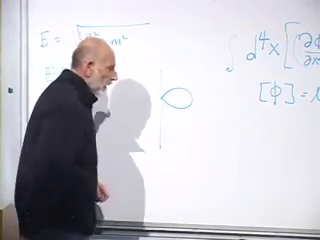
\includegraphics[width=0.72\textwidth]{lecture_03_figure_02.png}
\lectureframe{00:28:30.560}

\medskip
\begin{tikzpicture}[line width=0.8pt,scale=1.0]
  \draw[dashed] (-2.6,0) -- (0,0) -- (2.6,0);
  \fill (0,0) circle (0.055);
  \draw (0,0) .. controls (-0.85,0.7) and (-0.85,1.6) .. (0,1.6)
                .. controls (0.85,1.6) and (0.85,0.7) .. (0,0);
\end{tikzpicture}
\caption{標量自能推導過程中的黑板畫面，以及隨後對蝌蚪圖拓樸所作的保守示意重繪。截圖可清楚確認圈圖、相對論性與無質量能量公式，以及部分作用量；被遮住的係數與標示無法確認，因此不予呈現。}
\end{figure}

在頂點處，標量可以被吸收再發射，另外兩條線則從該點傳播後回到同一點。略去數值與組合因子，修正為
\begin{equation}
\delta m_\phi^2\sim \lambda G_\phi(0).
\end{equation}
在連續理論近似下，重合點的傳播子是無限大。有效理論不宣稱在任意短距離都適用，因此施加\(|\Delta|\geq\delta\)。於是
\begin{equation}
G_\phi(0)\longrightarrow G_\phi(\delta)sim\frac{1}{\delta^2},
\qquad
\delta m_\phi^2\sim\frac{\lambda}{\delta^2}sim\lambda\Lambda^2.
\end{equation}
這稱為二次發散，因為其中含有動量截止的二次方。動量空間的積分也會導出相同結論：過大的貢獻來自任意大的圈動量。最短尺度最終由大統一、量子重力，或尚未想到的其他物理設定，都不影響這項有效理論的判斷。

這就是精細調節問題。如果\(\delta\)極小，而\(\lambda\)並未小到異常的程度，輻射修正就會遠大於低能下觀測到的標量質量平方。如此一來，裸係數與圈修正必須精確抵消到許多位數，令人難以置信：
\begin{equation}
m_{\mathrm{physical}}^2
=m_{\mathrm{bare}}^2+\delta m_\phi^2.
\end{equation}
有質量傳播子也無法挽救這個情況。在造成發散的距離上，\(e^{-m|\Delta|}\simeq1\)。紫外圈圖在到達截止尺度之前，就早已不受質量影響。

\section{費米子的量綱與傳播子}

現在以相同的量綱分析處理狄拉克費米子。其自由作用量為
\begin{equation}
S_\psi=\int d^4x\,
\bar\psi\left(i\gamma^\mu\partial_\mu-m\right)\psi.
\end{equation}
伽馬矩陣是數值矩陣，且無量綱。動能項只含一個導數，因此
\begin{align}
1
&=L^4[\bar\psi]L^{-1}[\psi],\\
[\psi]=[\bar\psi]&=L^{-3/2}.
\end{align}
半整數次冪不必令人擔心；費米子在許多地方都會帶來半整數。

\begin{classroomqa}
\audiencequestion{從質量項推導\([\psi]\)不是比較簡單嗎？\lecturetimestamp{00:36:02}}
\lecturerresponse{是的。質量項給出\(L^4L^{-1}[\bar\psi\psi]=1\)，因此\([\bar\psi\psi]=L^{-3}\)，也就得到\([\psi]=L^{-3/2}\)。先從動能項推導，是因為這種推導在無質量理論中仍然適用，也能顯示為什麼費米子質量以\(m\)而非\(m^2\)的形式出現。}
\end{classroomqa}

兩個費米子場的乘積具有\(L^{-3}\)的量綱，因此講義以簡潔的量綱記號將無質量傳播子寫成
\begin{equation}
S(\Delta)\sim\frac{1}{|\Delta|^3}.
\end{equation}
恢復其矩陣結構後，洛倫茲協變性要求分子具有更精確的形式：
\begin{equation}
S_{ij}(\Delta)
\propto
\frac{\left(\gamma_\mu\Delta^\mu\right)_{ij}}
{\left(\Delta^2\right)^2}.
\end{equation}
分子多出一個長度冪次，因此分母含有間隔的四次方；整體量綱仍為\(L^{-3}\)。和標量情形一樣，費米子質量會抑制大間隔處的傳播，但不改變短距離的尺度行為。

\section{為什麼閉合費米子圈帶負號}

現在可以問，費米子圖能否抵消有問題的玻色子自能。標量蝌蚪圖的符號為正，至多乘上\(\pi\)的冪次或組合係數等正數值因子。閉合費米子圈則帶有相反的符號。

\begin{classroomqa}
\audiencequestion{費米子圈的負號和先前提到的完整一圈旋轉有關嗎？\lecturetimestamp{00:40:21}}
\lecturerresponse{它們都源於費米子相同的符號結構，但此處有用的證明是從交換反對稱性出發，而不是訴諸圈圖的幾何取向。將兩個圈各切開一處，交換全同粒子，再把線重新接起來。交換會使兩個圈變成一個圈，而且只有費米子會因此多出一個負號。}
\end{classroomqa}

這個論證值得完整說明。假設某個單圈圖的符號是\(\sigma\)，亦即正號或負號。兩個互不相連且相同的圈，其符號為
\begin{equation}
\sigma^2=+1.
\end{equation}
同時切開兩個圈後，會有兩個全同粒子在切口之間傳播。一般而言，玻色子的雙粒子波函數在交換下對稱，費米子的則反對稱：
\begin{align}
\Psi_B(x_1,x_2)&=+\Psi_B(x_2,x_1),\\
\Psi_F(x_1,x_2)&=-\Psi_F(x_2,x_1).
\end{align}
反對稱性也解釋了泡利不相容原理：若兩個費米子處於相同狀態，交換它們在物理上不會造成任何改變，但波函數必須反號，因此只能為零。

交換兩個粒子後，再把切開的線重新接起來。從拓樸上看，兩個圈已經變成一個。未交換時，雙圈振幅為正。交換之後，玻色子的振幅仍為正，費米子的振幅則反號。因此
\begin{equation}
\begin{aligned}
\operatorname{sign}(\text{closed boson loop})&=+1,\\
\operatorname{sign}(\text{closed fermion loop})&=-1.
\end{aligned}
\end{equation}
這是普遍的結論：每個獨立的閉合費米子圈都帶來一個\(-1\)因子。

\section{湯川圈圖}

回到標量質量。玻色子不能轉變成單一費米子，因為這會改變費米子數的奇偶性。最簡單的費米子修正是標量分裂成一對費米子與反費米子，兩者繞圈傳播後再重新結合。這種相互作用由湯川耦合描述：
\begin{equation}
\mathcal L_Y=-g\phi\bar\psi\psi.
\end{equation}
對希格斯而言，這些費米子可以是夸克或輕子。圖中有兩個相互作用頂點，因此會出現兩個\(g\)因子。

標量蝌蚪圖只有一個頂點；由於平移不變性只帶來時空體積因子，因此可以固定頂點的整體位置。湯川圈圖則有兩個頂點。我們可以固定其中一個的位置，或等價地固定兩者的平均位置，但仍須對它們的相對間隔\(\Delta\)積分。每個費米子傳播子都貢獻短距離因子\(1/|\Delta|^3\)，因此
\begin{equation}
\delta m_{\phi,F}^2
\sim
-g^2\int_{|\Delta|\geq\delta}d^4\Delta\,
\frac{1}{|\Delta|^6}.
\end{equation}

寫出兩個傳播子、間隔積分與兩個耦合之後，聽眾補上最後缺少的因子：負號。兩個傳播子閉合成費米子圈，因此整個原本為正的短距離積分要乘上\(-1\)。

量綱分析已足以確定發散程度。\(d^4\Delta\)帶來四個長度冪次，分母有六個，而唯一剩下的長度尺度是截止尺度：
\begin{equation}
\int_{|\Delta|\geq\delta}
\frac{d^4\Delta}{|\Delta|^6}
\sim\frac{1}{\delta^2}.
\end{equation}
用四維歐幾里得徑向座標可以明確寫出：
\begin{equation}
\int_{\delta}^{R}d^4\Delta\,\frac{1}{|\Delta|^6}
=2\pi^2\int_{\delta}^{R}dr\,\frac{r^3}{r^6}
=\pi^2\left(\frac{1}{\delta^2}-\frac{1}{R^2}\right).
\end{equation}
旋量跡與傳播子的正規化會改變係數，但不會改變截止尺度的二次方。\editorialnote{這個徑向積分具體呈現了講座中的量綱估算。它以歐幾里得距離表示，使正定性與紫外冪次計數一目了然。}

\begin{classroomqa}
\audiencequestion{反轉積分限或採用不同的積分限會改變符號嗎？\lecturetimestamp{00:51:06}}
\lecturerresponse{不會。這不是由積分限決定物理符號的一維有向積分，而是對四個分量積分；更明確地說，是對正的徑向測度積分。其紫外貢獻為正。負號完全來自閉合費米子圈。}
\end{classroomqa}

\begin{classroomqa}
\audiencequestion{湯川耦合\(g\)的量綱是多少？\lecturetimestamp{00:51:51}}
\lecturerresponse{在四維中，它是無量綱的。由於\([\phi]=L^{-1}\)與\([\bar\psi\psi]=L^{-3}\)，乘積\(\phi\bar\psi\psi\)的量綱為\(L^{-4}\)，恰好由\(d^4x\)抵消。}
\end{classroomqa}

因此，領先的費米子修正為
\begin{equation}
\delta m_{\phi,F}^2
\sim -C_F\frac{g^2}{\delta^2}
=-C_Fg^2\Lambda^2,
\end{equation}
其中\(C_F>0\)包含數值、自旋與多重度因子。標量圈的修正則具有相應形式：
\begin{equation}
\delta m_{\phi,B}^2
\sim+C_B\frac{\lambda}{\delta^2}
=+C_B\lambda\Lambda^2.
\end{equation}
我們還沒有解決精細調節問題，但已經找到一個不可或缺的條件：存在一項紫外發散程度相同、符號相反的貢獻。

\section{抵消所需的條件}

若彼此無關的耦合恰好滿足
\begin{equation}
C_B\lambda=C_Fg^2
\end{equation}
且精確度足以符合巨大尺度階層的要求，那將是非比尋常的巧合。講座以\(g^2=\lambda\)簡略表示這項條件，省略了依慣例與多重度而定的因子。真正的解決方案需要一種數學結構來強制這項關係，而不只是容許它成立。

這就是超對稱的動機。超對稱將玻色子與費米子聯繫起來，並限制其耦合，使之形成能抵消許多原本危險發散項的組合。這種抵消會在不同圖中一再出現，因為它源自對稱性，而不是逐圈調整參數的結果。

質量匹配同樣重要。若玻色子與費米子的質量完全相同，就能最緊密地配對兩者的完整傳播子。若質量略有差異，完整的有限結果便不會完全抵消，因為傳播子在康普頓波長相當的距離上有所不同。不過，兩者相同的短距離漸近行為仍能抵消發散部分：
\begin{equation}
\mathcal I_B(\Delta)-\mathcal I_F(\Delta)
\quad\hbox{may be finite as}\quad \Delta\to0,
\end{equation}
其中\(\mathcal I_B\)與\(\mathcal I_F\)分別表示納入頂點、分子與多重度後，完整的玻色子圈與費米子圈被積函數。兩者的傳播子本身量綱不同，因此並非直接相減。即使紫外項抵消，仍可能留下有限的殘餘項。這便為近似超對稱或破缺超對稱留下空間。質量完全相等時，抵消最為乾淨；若破缺受到充分控制，仍可能消除紫外災難，同時留下可觀測的質量劈裂。

因此，即使還沒寫出超對稱的代數，我們已經推導出超對稱的動機。整段推理如下：
\begin{equation}
\begin{gathered}
G_\phi(\Delta)\sim \Delta^{-2},
\qquad
\delta m_{\phi,B}^2\sim+C_B\lambda\Lambda^2,\\[0.4em]
S_\psi(\Delta)\sim \Delta^{-3},
\qquad
\delta m_{\phi,F}^2\sim-C_Fg^2\Lambda^2,\\[0.4em]
\text{symmetry-enforced matching}\\
\Longrightarrow\quad
\text{quadratic divergences cancel}.
\end{gathered}
\end{equation}
接下來要理解能強制這些關係成立的抽象對稱原理，並看幾個具體例子，了解它如何作用。
\chapter{從普通對稱性到格拉斯曼代數}

\lectureoverview{超對稱是一種對稱性，因此我們先回顧這個詞在量子力學中的意義。物理變換由作用於希爾伯特空間的么正算符表示；連續變換可由無窮小變換生成，而其交換子則編碼了變換的組合方式。真正的對稱性會保持能量不變，這等價於變換與哈密頓量對易。超對稱改變了所有熟悉例子共有的一項假設：它的生成元會將玻色子變為費米子，也會將費米子變為玻色子。構造這類生成元，自然會引出產生與湮滅算符、反對易子，以及奇元素平方為零的有限維格拉斯曼代數。}

\section{對稱性關聯不同的組態}

對稱性不只是裝飾性的規律，而是一種將一個物理組態與另一個組態關聯起來的操作。例如，左右反射會將兩隻手彼此對應。如果一個人及其周遭定律具有精確的左右對稱性，兩隻手的相應性質就會一致。更一般地說，由精確對稱性相連的物體或態，必須具有該對稱性所保持的物理量。在粒子物理學中，這通常意味著質量相等；在原子物理學中，則意味著同一轉動多重態中的態具有相同能量。

我們的目標是超對稱，但不妨先回顧轉動和平移等連續對稱性。超對稱在通常意義上是否為「連續」對稱性，這個問題本身就不容易回答。它的無窮小參數不是普通的可交換實數。最好將它視為連續對稱性的分次推廣；下文引入的格拉斯曼算術，足以讓這個說法在目前的討論中變得精確。\editorialnote{現代術語將超對稱描述為連續分次對稱性。這項限定說明了講座中的提醒：通常的連續與離散之分，並不完全適用於超對稱。}

\section{希爾伯特空間上的么正操作}

量子系統以態向量\(\ket{\psi}\)表示。物理對稱操作則以作用於該態的算符\(U\)表示：
\begin{equation}
\ket{\psi}\longmapsto U\ket{\psi}.
\end{equation}
對空間轉動而言，轉軸與轉角決定了\(U\)。如果一個態包含位於多個位置的粒子，變換後的右矢便代表這些粒子都位於各自旋轉後的位置。平移的作用方式類似：它將原態變為整個組態都已平移的態。

\begin{classroomqa}
\audiencequestion{態向量屬於一個往往是無限維的希爾伯特空間。我們轉動的是希爾伯特空間，還是普通的三維空間？\lecturetimestamp{00:04:20}}
\lecturerresponse{這兩種說法是在不同層次上描述同一個操作。么正變換作用於希爾伯特空間中的向量，表示組態在普通空間中的物理轉動。這不是字面上將抽象的希爾伯特空間作三維轉動，而是在希爾伯特空間中表示空間轉動。}
\end{classroomqa}

關鍵條件是么正性：
\begin{equation}
U^\dagger U=UU^\dagger=\mathbf 1,
\qquad
U^{-1}=U^\dagger.
\end{equation}
這會保持內積，因而保持機率：
\begin{equation}
\braket{U\psi}{U\psi}
=\bra{\psi}U^\dagger U\ket{\psi}
=\braket{\psi}{\psi}.
\end{equation}

\begin{figure}[H]
\centering
\includegraphics[width=0.56\textwidth]{lecture_04_figure_02.png}
\lectureframe{00:05:56.420}
\caption{黑板上先從變換後的態過渡到么正性條件。右矢與帶匕首的乘積清晰可見，但講者遮住了等式右側的部分；完整方程見下文推導。}
\end{figure}

嚴格來說，維格納定理也容許反么正對稱性，例如時間反演。本文所討論、與恆等變換連續相連的變換，則由么正算符表示。\editorialnote{反么正變換是標準的補充說明，不影響講座對轉動、平移或超對稱生成元的討論。}

\section{無窮小變換與生成元}

什麼都不做所對應的是\(U=\mathbf 1\)，而不是\(U=0\)。足夠小的變換與恆等變換只差一個對小參數呈線性的項。對於轉過小角度\(\epsilon\)的轉動，
\begin{equation}
U(\epsilon)=\mathbf 1+i\epsilon L+O(\epsilon^2).
\end{equation}
么正性在一階近似下要求
\begin{align}
U^\dagger U
&=\left(\mathbf 1-i\epsilon L^\dagger\right)
  \left(\mathbf 1+i\epsilon L\right)+O(\epsilon^2)\\
&=\mathbf 1+i\epsilon(L-L^\dagger)+O(\epsilon^2),
\end{align}
因此
\begin{equation}
L^\dagger=L.
\end{equation}
算符\(L\)就是無窮小生成元。

轉動需要三個生成元，分別對應三個獨立的軸：
\begin{equation}
L_x,\qquad L_y,\qquad L_z.
\end{equation}
繞任意軸\(\widehat{\bm n}\)的轉動由下式生成：
\begin{equation}
L_{\widehat{\bm n}}=\widehat{\bm n}\cdot\bm L.
\end{equation}

\begin{classroomqa}
\audiencequestion{繞\(x\)、\(y\)和\(z\)軸的生成元，可以相加來生成繞另一軸的轉動嗎？\lecturetimestamp{00:07:50}}
\lecturerresponse{可以。它們的線性組合能生成繞中間方向軸的轉動。三個獨立分量足以構成所有無窮小空間轉動。}
\end{classroomqa}

對轉動而言，這些生成元就是角動量的分量。這套記號也適用於更一般的情況，因為任何連續對稱性都可以在局部透過其生成元來理解。

\section{作為乘法表的交換子}

轉動生成元滿足
\begin{align}
[L_x,L_y]&=iL_z,&
[L_y,L_z]&=iL_x,&
[L_z,L_x]&=iL_y,
\end{align}
簡潔地寫成
\begin{equation}
[L_i,L_j]=i\epsilon_{ijk}L_k.
\end{equation}
兩個指標相同時，Levi-Civita 符號為零；對\(1,2,3\)的偶排列或奇排列，它分別等於\(+1\)或\(-1\)。關鍵的結構性質是封閉性：兩個生成元的交換子仍是生成元。

為什麼交換子能描述轉動的幾何？先繞\(x\)軸作一次小轉動，再繞\(y\)軸作一次小轉動，接著反向轉回\(x\)軸的轉動，最後反向轉回\(y\)軸的轉動。這些操作不會彼此抵消，因為繞不同軸的轉動不對易。

\begin{classroomqa}
\audiencequestion{這種不對易現象，可以用飛機的滾轉、俯仰和偏航來理解嗎？\lecturetimestamp{00:12:36}}
\lecturerresponse{可以。依序繞機體軸轉動，便能直接從幾何上看出改變操作順序會改變最終姿態。下文的代數正是這個熟悉事實的無窮小版本。}
\end{classroomqa}

令
\begin{equation}
U_x(\epsilon)=\mathbf 1+i\epsilon L_x,
\qquad
U_y(\delta)=\mathbf 1+i\delta L_y.
\end{equation}
由於算符從右向左作用於右矢，所述的操作順序可表示為
\begin{equation}
\mathcal C
=U_y^{-1}(\delta)U_x^{-1}(\epsilon)
 U_y(\delta)U_x(\epsilon).
\end{equation}

\begin{classroomqa}
\audiencequestion{為什麼反向操作可以寫成逆算符，而不是厄米共軛？\lecturetimestamp{00:13:25}}
\lecturerresponse{因為這些變換是么正的：\(U^\dagger=U^{-1}\)。對無窮小變換取逆，只需反轉一階項的符號：\(U_x^{-1}=\mathbf 1-i\epsilon L_x+O(\epsilon^2)\)。}
\end{classroomqa}

在黑板上計算這四個因子的乘積，成了全班一起投入的練習：所有關於\(\epsilon\)或\(\delta\)的一階項都抵消了，大家逐一追蹤混合項；一度出現的係數二混淆，也顯示算符順序很容易弄錯。整理後的二階結果是
\begin{align}
\mathcal C
&=\mathbf 1+\epsilon\delta[L_x,L_y]
  +O(\epsilon^2\delta,\epsilon\delta^2)\\
&=\mathbf 1+i\epsilon\delta L_z
  +O(\epsilon^2\delta,\epsilon\delta^2).
\end{align}
因此，這個閉合操作序列留下了一個繞\(z\)軸的小轉動，其轉角正比於\(\epsilon\delta\)。\editorialnote{經過課堂上的嘗試性計算後，這裡列出的乘法結果確定了操作順序與係數。若採用相反的序列約定，符號也會反轉；但殘餘變換由交換子決定這一結論不變。}

\begin{classroomqa}
\audiencequestion{如果改變反向操作的順序，乘積會變成恆等變換嗎？\lecturetimestamp{00:25:23}}
\lecturerresponse{如果每個變換都緊接在它自己的逆變換旁邊，成對的因子就會抵消。這個非平凡的交換子序列刻意將它們分開；它無法化為恆等變換，正是順序依賴性的表現。}
\end{classroomqa}

較長的乘積確實會更複雜，但沒有引入新的原理。

\begin{classroomqa}
\audiencequestion{如果生成元多於三個，或有許多小變換，會發生什麼事？\lecturetimestamp{00:25:34}}
\lecturerresponse{交換子會更多，計算也更繁複；但只要知道封閉代數，就能確定任意多個無窮小變換如何組合。有限變換可以由許多小變換組成。}
\end{classroomqa}

就此而言，交換子代數就是連續群在恆等元附近的乘法表。

\section{平移補足空間變換的例子}

空間平移由動量生成。依照講座採用的符號約定，
\begin{equation}
\begin{aligned}
T_x(a)&=\mathbf 1+iaP_x+O(a^2),\\
T_y(b)&=\mathbf 1+ibP_y+O(b^2),
\end{aligned}
\end{equation}
其中\(a\)和\(b\)代表距離，而不是角度。

兩個平移彼此對易。先將一點沿\(x\)方向移動，再沿\(y\)方向移動；接著反向移動\(x\)方向的平移，最後反向移動\(y\)方向的平移，該點便回到原點：
\begin{equation}
[P_i,P_j]=0.
\end{equation}

\begin{classroomqa}
\audiencequestion{平移或轉動物理物體，是否需要施力才能讓它開始和停止運動？\lecturetimestamp{00:28:45}}
\lecturerresponse{這裡所定義的操作並非如此。對稱變換是比較原始狀態與整個組態已平移或轉動後的數學狀態。它描述的不是動力學軌跡、加速度，也不是移動裝置時所做的功。}
\end{classroomqa}

轉動和平移不對易。先平移一個點，再令它繞原點轉動，接著沿原來的軸反向平移，最後反向轉回；該點不會回到原來的位置。混合代數關係為
\begin{equation}
[L_i,P_j]=i\epsilon_{ijk}P_k.
\end{equation}
這個關係表示動量本身在轉動下會如向量般變換。此處繁複的指標計算不是重點；一般性的結論是，歐幾里得空間的變換由轉動和平移生成元之間的交換子編碼。

\section{對稱性必須保持能量}

現在我們從變換的組合轉向動力學。如果\(U\)確實是系統的對稱變換，施行它就不能改變能量。設\(\ket{E}\)為能量本徵態：
\begin{equation}
H\ket{E}=E\ket{E}.
\end{equation}
等式右側的\(E\)是數；\(\ket{E}\)則是以該本徵值標記的向量。

\begin{figure}[H]
\centering
\begin{minipage}[t]{0.43\textwidth}
\centering
\includegraphics[width=\linewidth]{lecture_04_figure_03.png}
\lectureframe{00:34:38.239}
\end{minipage}
\hfill
\begin{minipage}[t]{0.50\textwidth}
\centering
\includegraphics[width=\linewidth]{lecture_04_figure_04.png}
\lectureframe{00:36:22.376}
\end{minipage}
\caption{變換後的右矢\(U\ket{E}\)與定義本徵值的方程\(H\ket{E}=E\ket{E}\)，分別呈現在連續的黑板畫面中。}
\end{figure}

如果\(U\)是對稱變換，那麼\(U\ket{E}\)也具有相同的本徵值：
\begin{equation}
HU\ket{E}=EU\ket{E}.
\end{equation}
由於\(E\)是純量，與\(U\)對易，因此可以使用原本的本徵值方程：
\begin{align}
HU\ket{E}
&=EU\ket{E}\\
&=UE\ket{E}\\
&=UH\ket{E}.
\end{align}
所以
\begin{equation}
(HU-UH)\ket{E}=0.
\end{equation}

\begin{classroomqa}
\audiencequestion{能否從第一個關係式重新推導一次？\lecturetimestamp{00:35:55}}
\lecturerresponse{從\(H\ket{E}=E\ket{E}\)開始。對稱性表示\(U\ket{E}\)具有相同能量，因此\(HU\ket{E}=EU\ket{E}\)。將純量\(E\)移過\(U\)，再以\(H\ket{E}\)取代\(E\ket{E}\)，然後相減，便得到\((HU-UH)\ket{E}=0\)。}
\end{classroomqa}

\begin{figure}[H]
\centering
\includegraphics[width=0.70\textwidth]{lecture_04_figure_05.png}
\lectureframe{00:38:51.066}
\caption{完整的黑板推導。彎曲的引導標記將等能量的陳述連到代入式\(E\ket{E}=H\ket{E}\)；最後一行是\((HU-UH)\ket{E}=0\)。}
\end{figure}

這個論證對每一個能量本徵態都成立。假設這些態構成完備基底，那麼對其中每個態作用後都得到零的算符，就是零算符：
\begin{equation}
[H,U]=0.
\end{equation}
這就是與時間無關的么正變換成為哈密頓量對稱變換的判準。

對無窮小變換而言，
\begin{equation}
U(\epsilon)=\mathbf 1+i\epsilon L_i+O(\epsilon^2),
\end{equation}
恆等算符本來就與\(H\)對易，因此每個生成元都必須滿足
\begin{equation}
[L_i,H]=0.
\end{equation}

\begin{figure}[H]
\centering
\includegraphics[width=0.47\textwidth]{lecture_04_figure_06.png}
\lectureframe{00:42:14.296}
\caption{黑板上精簡列出的對稱性判準：\([U,H]=0\)，接著是其生成元形式；後者依據部分模糊的下標整理為\([L_i,H]=0\)。}
\end{figure}

如果\(L_i\)沒有顯含時間，海森堡方程給出
\begin{equation}
\frac{dL_i}{dt}
=i[H,L_i]=0
\qquad(\hbar=1).
\end{equation}
因此，對稱性生成元是守恆荷。空間平移對稱性導出動量守恆；轉動對稱性導出角動量守恆。\editorialnote{顯式時間導數的條件是標準的補充說明；講座陳述守恆律時，已隱含了這項條件。}

\section{變換整個物理系統}

如果只變換裝置的一部分，「轉動是對稱性」這句話就可能遭到誤用。自由自旋可以旋轉而不改變能量。然而，若將它置於固定磁場中，卻只旋轉自旋，其塞曼能量就會改變。這不代表轉動對稱性不成立，而是因為自旋相對於磁場轉動時，磁場仍保持固定。若讓自旋和磁場一起轉動，或是外加磁場本身在該操作下保持不變，能量就不會改變。

氫原子也有同樣的問題。只平移電子而讓質子保持不動，會改變兩者的距離，因而改變庫侖能量。平移對稱性作用於完整的電子—質子系統，讓兩者移動相同的距離。

\begin{classroomqa}
\audiencequestion{外部場本身也必須具有該對稱性嗎？\lecturetimestamp{00:43:09}}
\lecturerresponse{固定的外部場必須已在該操作下保持不變，或者外部場必須和系統其他部分一起變換。自旋相對於未轉動的磁場所作的轉動，形成的是不同的物理組態，並非整個裝置經對稱變換後的組態。}
\end{classroomqa}

原子中的轉動簡併是一個清楚的正面例子。對固定角動量\(l\)而言，轉動會混合磁量子數為
\begin{equation}
m=-l,-l+1,\ldots,l.
\end{equation}
的態。在沒有外加磁場或電場時，多重態中的所有成員能量相同：
\begin{equation}
E_{l,m}=E_l.
\end{equation}
對稱性將不同的態彼此關聯，並使它們具有簡併能階。

\section{超對稱改變了什麼}

迄今討論的各種熟悉對稱性，都保留了玻色子與費米子的區別。轉動會將一個電子變為另一個電子，而不會將它變成光子。色旋轉會混合夸克的三種顏色，但不會將夸克變成膠子。普通的內部對稱性和時空對稱性可以混合不同分量或量子數標籤，但它們的生成元是玻色性的，不會改變費米子宇稱。

超對稱則不同：
\begin{equation}
Q\ket{B}\sim\ket{F},
\qquad
Q\ket{F}\sim\ket{B}.
\end{equation}
它的多重態跨越了玻色子與費米子之間的界線。在精確的超對稱理論中，同一多重態中的夥伴粒子質量相同。這正是前幾講所要求的配對：相互匹配的玻色子圈圖與費米子圈圖，可以抵消標量質量受到的大幅紫外修正。這種結構難以直觀理解，因為沒有普通的空間運動能讓整數自旋態變成半整數自旋態。因此，接下來我們採用代數方法。

\section{超荷的簡單模型}

設\(A,A^\dagger\)為玻色子的湮滅與產生算符，\(C,C^\dagger\)為費米子的湮滅與產生算符。交換兩種粒子的單粒子態，最簡單的厄米算符為
\begin{equation}
Q=C^\dagger A+A^\dagger C.
\end{equation}
第一項湮滅一個玻色子並產生一個費米子；第二項則湮滅一個費米子並產生一個玻色子。若\(Q\)作用於單玻色子態，\(A^\dagger C\)項會消失，因為沒有費米子可供湮滅；此時由\(C^\dagger A\)完成轉換。作用於單費米子態時，兩項的作用則互換。

\begin{classroomqa}
\audiencequestion{這種構造會產生一個同時為玻色子與費米子疊加態的單一粒子嗎？\lecturetimestamp{00:52:37}}
\lecturerresponse{\(Q\)是算符，不是態。它作用於純玻色態時會產生費米態；作用於純費米態時則會產生玻色態。若它線性作用於原本已是一般疊加態的態，便會產生另一個疊加態，就像任何線性算符一樣。}
\end{classroomqa}

接著來檢驗真空態。由於兩個湮滅算符作用於真空態都會得到零，
\begin{equation}
A\ket{0}=0,\qquad C\ket{0}=0,
\end{equation}
因此
\begin{equation}
Q\ket{0}=0.
\end{equation}
結果是零向量，而不是另一個真空態。

這個模型刻意採取示意性的簡化。一個自旋為零的玻色子可以轉換成自旋二分之一費米子的任一自旋分量，因此生成元本身需要帶有旋量指標：
\begin{equation}
Q_\alpha\ket{B}\sim\ket{F_\alpha}.
\end{equation}
在講座簡化的雙分量圖像中，
\begin{equation}
Q_\alpha\ket{F_\beta}\sim\delta_{\alpha\beta}\ket{B}.
\end{equation}

\begin{classroomqa}
\audiencequestion{自旋為零的玻色子只有一個自旋分量，自旋二分之一的費米子卻有兩個；這種情況下，態空間的維度如何能相符？\lecturetimestamp{00:55:02}}
\lecturerresponse{單一不帶指標的\(Q\)並不足夠。還有旋量分量\(Q_\alpha\)，每個分量都能產生一個費米子自旋分量。超荷本身帶有半單位自旋，因為它會使自旋改變半個單位。}
\end{classroomqa}

\(Q_\alpha\)是費米性算符，更精確地說，是格拉斯曼奇算符。每一項都含有奇數個費米子算符，因此會反轉費米子宇稱。一般可觀測量則是偶的。必須區分奇超荷與奇變換參數：有限的超對稱變換由\(\epsilon^\alpha Q_\alpha+\bar\epsilon_{\dot\alpha}\bar Q^{\dot\alpha}\)這類偶組合構成，其中\(\epsilon\)和\(Q\)都是奇的。\editorialnote{講座非正式地將生成元稱為格拉斯曼數。更精確地說，超荷是奇算符，反對易參數則是格拉斯曼數；兩者的乘積為偶，可以出現在有限變換中。}

\section{玻色子與費米子的算符代數}

對以\(i,j\)標記的玻色模式，
\begin{align}
[A_i,A_j]&=0,&
[A_i^\dagger,A_j^\dagger]&=0,&
[A_i,A_j^\dagger]&=\delta_{ij}.
\end{align}
這些標記可以代表動量、位置、自旋，或任何完備的單粒子基底。由於產生算符彼此對易，
\begin{equation}
A_i^\dagger A_j^\dagger\ket{0}
=A_j^\dagger A_i^\dagger\ket{0}.
\end{equation}
雙玻色子態在交換兩個粒子時保持對稱。

費米子算符滿足反對易關係：
\begin{align}
\{C_i,C_j\}&=0,&
\{C_i^\dagger,C_j^\dagger\}&=0,&
\{C_i,C_j^\dagger\}&=\delta_{ij},
\end{align}
其中
\begin{equation}
\{X,Y\}=XY+YX.
\end{equation}
對單一模式而言，
\begin{equation}
\{C^\dagger,C^\dagger\}=2(C^\dagger)^2=0,
\end{equation}
因此
\begin{equation}
(C^\dagger)^2=0.
\end{equation}
這個算符本身不為零，但它的平方為零。它可以在該模式中產生一個費米子；再作用一次就會得到零。這就是泡利不相容原理的算符表述。

對不同的標記而言，
\begin{equation}
C_i^\dagger C_j^\dagger\ket{0}
=-C_j^\dagger C_i^\dagger\ket{0},
\end{equation}
這體現了雙費米子態的反對稱性。代數上的替換關係
\begin{equation}
\begin{gathered}
\text{bosons: commutators}\\
\Updownarrow\\
\text{fermions: anticommutators}
\end{gathered}
\end{equation}
則編碼了統計性質的差異。

許多玻色子可以佔據同一個模式。因此，當光子佔據數很大時，其行為可以類似具有普通數值振幅的經典電磁場。費米子不能在同一模式中不斷累積，而奇費米場也不會取得普通的可交換經典值。因此，描述費米子時需要採用不同的算術。

\section{格拉斯曼數與宇稱}

普通數彼此可交換：
\begin{equation}
\alpha_i\alpha_j=\alpha_j\alpha_i.
\end{equation}
格拉斯曼生成元彼此反交換：
\begin{equation}
\theta_i\theta_j=-\theta_j\theta_i.
\end{equation}
令\(i=j\)，並考慮滿足\(2\neq0\)的數系，便得到
\begin{equation}
\theta_i^2=0.
\end{equation}
\(\theta_i\)不能取六或七這類普通數值。這些符號構成一種用來追蹤費米子符號的代數。

普通係數與格拉斯曼生成元彼此可交換：
\begin{equation}
\alpha\theta_i=\theta_i\alpha.
\end{equation}

\begin{classroomqa}
\audiencequestion{普通數乘上格拉斯曼數會得到什麼類型的物件？\lecturetimestamp{01:12:32}}
\lecturerresponse{結果仍是格拉斯曼奇元素。乘上普通係數只會改變尺度，不會改變宇稱。這些生成元所張成的空間，是以普通數為係數的向量空間。}
\end{classroomqa}

這個代數具有\(\mathbb Z_2\)宇稱。普通係數與偶數個生成元的乘積都是偶元素；單一生成元或奇數個生成元的乘積則是奇元素：
\begin{equation}
\begin{aligned}
\text{even}\cdot\text{even}&=\text{even},\\
\text{even}\cdot\text{odd}&=\text{odd},\\
\text{odd}\cdot\text{odd}&=\text{even}.
\end{aligned}
\end{equation}

\begin{classroomqa}
\audiencequestion{這類似實數與虛數的乘法規則嗎？或者，它像引入\(i\)那樣，是一種推廣嗎？\lecturetimestamp{01:14:25}}
\lecturerresponse{這是算術的一種推廣，但不宜過度延伸這個類比。虛數仍然可交換，並滿足\(i^2=-1\)；格拉斯曼奇量則反交換，且平方為零。兩者雖有相同的奇偶乘法模式，代數結構卻並不相同。}
\end{classroomqa}

像\(\theta_1\theta_2\)這樣的乘積是偶元素，並且與格拉斯曼代數中的每個齊次元素可交換，但它不是普通數。它本身不為零，然而
\begin{equation}
(\theta_1\theta_2)^2=0.
\end{equation}

\begin{classroomqa}
\audiencequestion{既然\(\theta_1\theta_2\)是偶的，為什麼它不只是普通數？\lecturetimestamp{01:17:36}}
\lecturerresponse{偶宇稱表示它在分次代數中可交換，但不表示它是實數或複數純量。它具有冪零性，立刻就能與非零普通數區分開來。}
\end{classroomqa}

\section{格拉斯曼變數的函數}

只有一個生成元時，任何多項式都只會有零階與一階項：
\begin{equation}
f(\theta)=\alpha+\beta\theta.
\end{equation}
所有符合\(n\geq2\)的冪\(\theta^n\)都為零。有兩個生成元時，最一般的元素為
\begin{equation}
f(\theta_1,\theta_2)
=\alpha+\beta_1\theta_1+\beta_2\theta_2
+\gamma\theta_1\theta_2.
\end{equation}
將最後一個單項式的因子順序反轉，符號也會改變：
\begin{equation}
\theta_2\theta_1=-\theta_1\theta_2.
\end{equation}

\begin{classroomqa}
\audiencequestion{將\(\theta_1\)乘以係數\(\beta\)，會產生第三個獨立的格拉斯曼變數嗎？\lecturetimestamp{01:18:39}}
\lecturerresponse{不會。這只會得到\(\theta_1\)所張成空間中的另一個向量，並不會產生新的基底生成元。只有兩個獨立生成元時，所有奇線性項都可寫成\(\beta_1\theta_1+\beta_2\theta_2\)。}
\end{classroomqa}

三個生成元的有序基底為
\begin{equation}
1,\quad
\theta_1,\theta_2,\theta_3,\quad
\theta_1\theta_2,\theta_1\theta_3,\theta_2\theta_3,\quad
\theta_1\theta_2\theta_3.
\end{equation}
一般而言，\(n\)個生成元會產生\(2^n\)個有序基底單項式。有限個格拉斯曼生成元的任何解析函數都會截斷成這類多項式，因為生成元重複出現時乘積為零。\editorialnote{\(2^n\)維基底明確呈現了講座以一、二、三個生成元建構出的規律。}

\section{格拉斯曼微分}

對單一變數，定義
\begin{equation}
\frac{\partial}{\partial\theta}\alpha=0,
\qquad
\frac{\partial}{\partial\theta}\theta=1,
\end{equation}
使得
\begin{equation}
\frac{\partial}{\partial\theta}
(\alpha+\beta\theta)=\beta.
\end{equation}
對兩個變數，採用左導數，並保持標準順序\(\theta_1\theta_2\)：
\begin{align}
\frac{\partial^L f}{\partial\theta_1}
&=\beta_1+\gamma\theta_2,\\
\frac{\partial^L f}{\partial\theta_2}
&=\beta_2-\gamma\theta_1.
\end{align}
第二行的負號來自奇導數必須先越過\(\theta_1\)，才能對\(\theta_2\)微分。

這可由分次乘法法則表達。若\(A\)的宇稱為\(|A|\in\{0,1\}\)，則
\begin{equation}
\frac{\partial^L}{\partial\theta}(AB)
=\left(\frac{\partial^L A}{\partial\theta}\right)B
+(-1)^{|A|}A
\left(\frac{\partial^L B}{\partial\theta}\right).
\end{equation}
這個法則的形式大致與普通乘法法則相同，但多了反交換性所要求的符號。格拉斯曼積分也可以定義；由於函數空間是有限維的，它可歸結為一個簡短的規則表。講座將那個表留待之後介紹。

\section{指數謎題的解答}

若只有一個格拉斯曼生成元，且普通係數為\(a\)，則
\begin{equation}
e^{a\theta}
=1+a\theta,
\end{equation}
因為所有更高次冪都為零。含有同一生成元的兩個指數滿足
\begin{align}
e^{a\theta}e^{b\theta}
&=(1+a\theta)(1+b\theta)\\
&=1+(a+b)\theta\\
&=e^{(a+b)\theta}.
\end{align}

接著，大家嘗試使用不同的生成元。直接相乘可得
\begin{equation}
e^{\theta_1}e^{\theta_2}
=(1+\theta_1)(1+\theta_2)
=1+\theta_1+\theta_2+\theta_1\theta_2.
\end{equation}
一開始，黑板上的展開式似乎暗示\(\theta_1+\theta_2\)的平方會給出最後一項。此時一位聽眾指出了符號錯誤：
\begin{equation}
(\theta_1+\theta_2)^2
=\theta_1^2+\theta_1\theta_2
 +\theta_2\theta_1+\theta_2^2
=0.
\end{equation}

\begin{classroomqa}
\audiencequestion{平方項會不會因為含有\(\theta_1\theta_2+\theta_2\theta_1\)而抵消？\lecturetimestamp{01:24:00}}
\lecturerresponse{會。這項修正改變了結論：\(e^{\theta_1+\theta_2}=1+\theta_1+\theta_2\)，而有序乘積\(e^{\theta_1}e^{\theta_2}\)也含有\(\theta_1\theta_2\)。樸素的指數加法公式不適用於不同的反交換指數。}
\end{classroomqa}

這並不矛盾。即使是普通矩陣，也只有在\(A\)與\(B\)對易時，才滿足\(e^Ae^B=e^{A+B}\)。此處
\begin{equation}
[\theta_1,\theta_2]
=\theta_1\theta_2-\theta_2\theta_1
=2\theta_1\theta_2.
\end{equation}
這個交換子為偶，且與兩個生成元都對易，因此 Baker–Campbell–Hausdorff 級數會終止：
\begin{equation}
e^{\theta_1}e^{\theta_2}
=\exp\left(
\theta_1+\theta_2+\frac12[\theta_1,\theta_2]
\right)
=e^{\theta_1+\theta_2+\theta_1\theta_2}.
\end{equation}
右側的指數是冪零的，因此恰好展開為
\(1+\theta_1+\theta_2+\theta_1\theta_2\)。\editorialnote{這項 BCH 計算解答了講座現場留下的問題。講座正確地發現樸素公式不成立，但在指出缺少的交換子項之前便已結束。}

\begin{classroomqa}
\audiencequestion{\(1+\theta_1\)是什麼類型的數？普通部分和格拉斯曼部分可以相加嗎？\lecturetimestamp{01:26:16}}
\lecturerresponse{這是格拉斯曼代數中的非齊次元素，包含偶部分\(1\)與奇部分\(\theta_1\)。這類和是允許的，但既不是普通純量，也不是齊次奇元素。}
\end{classroomqa}

接近結尾時，講座又檢驗了另一個看似矛盾的結果：
\begin{equation}
(\theta_1+\theta_2)^2=0.
\end{equation}
這不代表\(\theta_1\theta_2=0\)，因為兩個交叉項是彼此抵消，而不是各自為零。

\begin{classroomqa}
\audiencequestion{如果每個奇 Grassmann 元素的平方都為零，是否表示任意兩個 Grassmann 生成元的乘積也都為零？\lecturetimestamp{01:32:19}}
\lecturerresponse{不是。方程式 \((\theta_1+\theta_2)^2=0\) 表示 \(\theta_1\theta_2+\theta_2\theta_1=0\)。這證明的是反對易性，並不表示任一種排列下的乘積為零。不同的生成元相乘，結果可以不為零。}
\end{classroomqa}

\begin{classroomqa}
\audiencequestion{我們寫下這些指數函數時，是否假設採用通常的冪級數定義？\lecturetimestamp{01:34:42}}
\lecturerresponse{是的，而且這個定義是自洽的，因為每個級數都會終止。失效的不是指數函數本身，而是對非對易的 \(A\) 與 \(B\)，未經論證便套用恆等式 \(e^Ae^B=e^{A+B}\)。對易子修正項使合成律恢復正確。}
\end{classroomqa}

這樣以探索性的方式收尾恰如其分。從普通對稱性出發，我們由酉變換走到生成元與對易子；從超對稱性出發，我們由奇生成元走到反對易變數。在這兩種情形中，乘法律都是核心。對轉動而言，它體現在 \([L_i,L_j]\)；對 Grassmann 指數而言，它則體現在阻止直接相加的對易子項中。這套代數雖然陌生，卻自洽而有限，恰好適用於超對稱性所要求的費米子變換。

\chapter{超荷、閉合與超空間}

\lectureoverview{超對稱之所以困難，不在於規則繁多，而在於這些規則把普通物理學中分開處理的觀念結合在一起。我們從格拉斯曼變數談起：它們的奇元素彼此反交換，而以這些變數為自變數的函數只會有有限項。格拉斯曼變數的微分代數，接著提供了奇對稱生成元的模型。玻色振子與費米振子構成最簡單的超荷：這些超荷的反對易子就是哈密頓量，因此玻色子與費米子的互換，和時間平移密不可分。同一代數也能以幾何方式表示：在稱為超空間的擴展時空中，沿格拉斯曼方向平移。}

\section{為什麼前進之前必須先退一步}

超對稱是物理學中最抽象的構造之一。它和旋轉、平移一樣是一種對稱性，但若不擴展座標的概念，就無法將它納入普通時空。它的自然參數是格拉斯曼量：這些物件可以相加、相乘，卻是反交換而非交換。

因此，直接處理最後的代數並不恰當。我們會先讓奇數的運算變得容易使用，再回顧普通連續對稱性如何組織，最後才把兩種觀念結合起來。這條路雖然較長，但每一步都為下一步鋪路。

\section{實用形式的格拉斯曼代數}

\subsection{奇元素與偶元素}

令 \(\epsilon_i\) 表示彼此獨立的格拉斯曼生成元。它們滿足
\begin{equation}
\epsilon_i\epsilon_j=-\epsilon_j\epsilon_i,
\qquad
\{\epsilon_i,\epsilon_j\}=0.
\end{equation}
令 \(i=j\)，便得到
\begin{equation}
2\epsilon_i^2=0,
\qquad
\epsilon_i^2=0,
\end{equation}
這些關係在實數或複數上成立。生成元本身不為零；為零的只有它的平方。

每個齊次元素都有奇偶性。含有奇數個格拉斯曼生成元的乘積是奇的，含有偶數個的乘積則是偶的：
\begin{align}
\text{odd}\times\text{odd}&=\text{even},\\
\text{odd}\times\text{even}&=\text{odd},\\
\text{even}\times\text{even}&=\text{even}.
\end{align}
偶元素與齊次元素交換，兩個奇元素則反交換。因此，當 \(n\) 為偶時，
\begin{equation}
n\epsilon_i=\epsilon_i n,
\qquad
\epsilon_i\epsilon_j=-\epsilon_j\epsilon_i,
\end{equation}

偶元素不一定是普通的實數或複數。例如，乘積 \(\epsilon_1\epsilon_2\) 是偶元素且為冪零。普通數構成代數中的純量部分；偶元素的乘積則提供其他可交換的元素。

\begin{classroomqa}
\audiencequestion{格拉斯曼代數和格拉斯曼數有區別嗎？還是兩者指的是同一回事？\lecturetimestamp{00:06:45}}
\lecturerresponse{格拉斯曼數是代數中的元素；格拉斯曼代數則是由這些元素，以及它們的加法和乘法規則所構成。因此，寬鬆地說兩者指的是同一個對象也可以，但區分運算的對象與運算規則仍有助於理解。}
\end{classroomqa}

\subsection{函數的展開會終止}

單一格拉斯曼變數的函數只有兩種可能的冪次：
\begin{equation}
f(\epsilon)=a+b\epsilon.
\end{equation}
不會有 \(\epsilon^2\) 項。若有兩個彼此獨立的生成元，
\begin{equation}
f(\epsilon_1,\epsilon_2)
=a+b_1\epsilon_1+b_2\epsilon_2+c\epsilon_1\epsilon_2.
\end{equation}
展開在兩個生成元都出現後便會終止。對於 \(n\) 個彼此獨立的生成元，有序單項式構成一組 \(2^n\) 維基底：
\begin{equation}
1,\quad
\epsilon_i,\quad
\epsilon_i\epsilon_j,\quad
\ldots,\quad
\epsilon_1\epsilon_2\cdots\epsilon_n.
\end{equation}
\editorialnote{有限的 \(2^n\) 維情形，概括了單一與兩個生成元的例子。也可以定義含有無限多個生成元的格拉斯曼代數，但這裡使用的多項式都只涉及有限個生成元。}

將兩個實生成元組成複數對 \(\theta,\bar\theta\) 後，一般函數可依選定的順序寫成
\begin{equation}
f(\theta,\bar\theta)
=a+\bar b\,\theta+\bar\theta\,b+c\,\bar\theta\theta.
\end{equation}
上方的橫線表示此處採用的複數對記號。若將最後兩個因子的順序顛倒，符號就會改變：
\begin{equation}
\bar\theta\theta=-\theta\bar\theta.
\end{equation}

通常，我們會為整個函數指定確定的奇偶性。若 \(f\) 為偶，則 \(a\) 和 \(c\) 為偶，\(b\) 和 \(\bar b\) 為奇。若 \(f\) 為奇，奇偶性便全部對調。係數本身可以屬於更大的格拉斯曼代數，只要它們不依賴於展開所用的那些特定變數。

\begin{classroomqa}
\audiencequestion{格拉斯曼變數可以代入三角函數或其他解析函數嗎？\lecturetimestamp{00:11:06}}
\lecturerresponse{可以，但冪級數很快就會終止。對單一奇生成元而言，
\[
\sin\epsilon=\epsilon,\qquad
\cos\epsilon=1,\qquad
e^\epsilon=1+\epsilon.
\]
函數仍沿用熟悉的名稱，但可用的冪次太少，無法呈現一般解析函數的複雜性。}
\end{classroomqa}

\section{微分就是符號的整理}

我們採用左格拉斯曼導數。它的局部定義規則為
\begin{equation}
\partial_\theta a=0,
\qquad
\partial_\theta(\theta B)=B,
\end{equation}
只要 \(a\) 和 \(B\) 不依賴 \(\theta\)，上述關係就成立。微分前，先將相關的 \(\theta\) 移到左側。每當它越過另一個奇因子，符號就會改變。

例如，若 \(b\) 為奇，
\begin{equation}
b\theta=-\theta b,
\qquad
\partial_\theta(b\theta)=-b.
\end{equation}
導數本身沒有任何神祕之處。負號是在微分之前、重新排列奇因子時產生的。

\subsection{雙變數的計算}

回到
\begin{equation}
f(\theta,\bar\theta)
=a+\bar b\,\theta+\bar\theta\,b+c\,\bar\theta\theta.
\end{equation}
先假設 \(f\) 為偶。於是 \(\bar b\) 為奇，\(c\) 為偶。重新排列含有 \(\theta\) 的項：
\begin{align}
\bar b\,\theta&=-\theta\bar b,\\
c\,\bar\theta\theta&=-\theta c\,\bar\theta.
\end{align}
因此
\begin{equation}
\partial_\theta f=-\bar b-c\bar\theta.
\end{equation}

若 \(f\) 為奇，則 \(\bar b\) 為偶，\(c\) 為奇。第一項不必越過任何奇係數；最後一項中的 \(\theta\) 則會越過兩個奇因子：\(c\) 和 \(\bar\theta\)。兩個負號彼此抵消：
\begin{equation}
\partial_\theta f=\bar b+c\bar\theta.
\end{equation}

\begin{classroomqa}
\audiencequestion{為什麼偶函數的例子中，留下的兩項都帶有負號？\lecturetimestamp{00:16:49}}
\lecturerresponse{第一個負號來自 \(\theta\) 越過奇係數 \(\bar b\)。在最後一項中，\(c\) 是偶的，但 \(\theta\) 必須越過奇變數 \(\bar\theta\)。每次重新排列都越過一個奇因子，因此各產生一個負號。}
\end{classroomqa}

答案取決於排列的約定，但數學本身不受影響。若一開始寫成 \(c\theta\bar\theta\) 而非 \(c\bar\theta\theta\)，顯示的係數就會差一個負號，導數公式也會相應改變。

\begin{classroomqa}
\audiencequestion{最後一項能否改寫成 \(\theta\) 和 \(\bar\theta\) 順序相反的形式？這樣產生的符號有更深層的意義嗎？\lecturetimestamp{00:18:50}}
\lecturerresponse{可以採用任一種順序，但交換兩個奇變數會改變符號。這個負號可以併入係數 \(c\)。在目前這個階段，這只是整理符號的問題：順序會影響正負號，奇偶性則不會改變；符號改變也絕不會把奇物件變成偶物件。當同樣的符號規則用來確保費米子統計和超對稱成立時，它才顯出物理意義。}
\end{classroomqa}

\begin{classroomqa}
\audiencequestion{係數 \(a,b,c\) 就只是取自複數域嗎？\lecturetimestamp{00:20:47}}
\lecturerresponse{若所需奇偶性為偶，係數可以是普通複數；也可以含有選定的 \(\theta,\bar\theta\) 以外的生成元。通常，所考慮的代數包含所有複數純量，以及一組選定的奇生成元與它們的乘積。}
\end{classroomqa}

\begin{classroomqa}
\audiencequestion{偶函數與奇函數的導數看起來互為相反數。這是一般性的對稱關係嗎？\lecturetimestamp{00:22:31}}
\lecturerresponse{不一定。符號是依照各係數的奇偶性，以及運算時越過了多少個奇因子逐步決定的。有時兩個結果恰好互為相反數，但可靠的規則更簡單：每交換兩個奇物件，就會多出一個負號。}
\end{classroomqa}

\subsection{座標與導數作為算符}

有一個很有啟發性的普通情形可供類比。令乘以 \(x\) 和對 \(x\) 微分這兩個運算作用於任意函數 \(g(x)\)，則
\begin{align}
\partial_x\!\left(xg\right)&=g+xg',\\
x\partial_xg&=xg',
\end{align}
所以
\begin{equation}
[\partial_x,x]g=g.
\end{equation}
由於這對任意 \(g\) 都成立，
\begin{equation}
[\partial_x,x]=1.
\end{equation}
取 \(p=-i\partial_x\)，便得到熟悉的位置與動量代數；這裡採用 \(\hbar=1\) 的單位制。

格拉斯曼變數的類比關係使用反對易子。令
\begin{equation}
f(\theta)=a+\theta b,
\end{equation}
其中 \(a\) 為偶、\(b\) 為奇，因此 \(f\) 為偶。先看
\begin{equation}
\theta\partial_\theta f=\theta b.
\end{equation}
再看相反的運算順序：
\begin{align}
\partial_\theta(\theta f)
&=\partial_\theta(\theta a+\theta^2b)\\
&=a.
\end{align}
將兩種順序的結果相加，便得到原函數：
\begin{equation}
\left(\partial_\theta\theta+\theta\partial_\theta\right)f
=a+\theta b=f.
\end{equation}
因此
\begin{equation}
\boxed{\{\partial_\theta,\theta\}=1.}
\end{equation}
導數 \(\partial_\theta\) 本身是奇的。這就是它與奇座標之間的正則關係採用反對易子的原因。

\begin{classroomqa}
\audiencequestion{可以使用同時含有偶部分和奇部分的函數，而不指定確定的奇偶性嗎？\lecturetimestamp{00:31:05}}
\lecturerresponse{這類非齊次元素可以構造出來，但計算通常會分別以齊次的偶物件和奇物件進行。指定確定的奇偶性，能讓分次乘積中的符號一目了然；混合物件則拆成偶部分與奇部分來處理。}
\end{classroomqa}

\begin{classroomqa}
\audiencequestion{在普通對易子的計算中，測試函數 \(g(x)\) 必須是奇函數嗎？\lecturetimestamp{00:31:45}}
\lecturerresponse{不必。它是普通可交換座標的普通函數。引入它只是為了說明算符恆等式 \([\partial_x,x]=1\) 如何證明，接著再以格拉斯曼變數對 \(\partial_\theta,\theta\) 重複同樣的論證。}
\end{classroomqa}

\begin{classroomqa}
\audiencequestion{獨立格拉斯曼生成元的數目有限制嗎？\lecturetimestamp{00:32:16}}
\lecturerresponse{代數上沒有上限。對 \(n\) 個生成元而言，基底有 \(2^n\) 個單項式，因此整理符號的工作會迅速增加，但此構造適用於任何有限的 \(n\)。}
\end{classroomqa}

\subsection{積分}

單一格拉斯曼變數的積分定義為
\begin{equation}
\int d\theta\,1=0,
\qquad
\int d\theta\,\theta=1.
\end{equation}
因此，對於 \(f(\theta)=a+\theta b\)，
\begin{equation}
\int d\theta\,f(\theta)=b=\partial_\theta f(\theta).
\end{equation}
積分與微分會提取相同的分量。這稱為貝雷津積分。這種歸一化方式是最簡單、且與平移不變性及格拉斯曼分部積分相容的選擇。\editorialnote{這些分量規則精確表達了講義中「格拉斯曼積分與微分是同一種運算」的說法。}

\section{以普通對稱性為基準}

考慮一個連續么正群，其厄米生成元為 \(G_i\)。在單位元附近，
\begin{equation}
U(\alpha)=\mathbf 1+i\alpha^iG_i+O(\alpha^2),
\end{equation}
其中 \(\alpha^i\) 是普通的可交換參數。無窮小乘法的規則由李代數描述：
\begin{equation}
[G_i,G_j]=i f_{ij}{}^{k}G_k.
\end{equation}
常數 \(f_{ij}{}^k\) 稱為結構常數。所謂閉合，是指任意兩個生成元的對易子都會回到代數中，成為既有生成元的線性組合。

對於轉動，
\begin{equation}
[L_i,L_j]=i\varepsilon_{ijk}L_k.
\end{equation}
三個厄米分量可組合成非厄米的升降算符：
\begin{equation}
L_\pm=L_x\pm iL_y,
\end{equation}
它們會使磁量子數 \(m\) 增加或減少一。複數線性組合雖然方便，但不會改變底層物理生成元的厄米性。

在一般基底下，\(f_{ij}{}^k\) 只有前兩個指標必須反對稱。對於具有不變正交度量的緊緻李代數，可以降低最後一個指標，並選擇適當的約定，使 \(f_{ijk}\) 完全反對稱，就如同轉動代數的情形。\editorialnote{這個限定說明，對易子的反對稱性普遍成立；熟悉的轉動基底還具有更強的性質。}

若要讓 \(G_i\) 成為時間無關系統的對稱性生成元，就必須有
\begin{equation}
[H,G_i]=0.
\end{equation}
等價地說，\(G_i\) 會將每個能量本徵空間映射到自身。若系統沒有顯式的時間依賴，海森堡方程給出
\begin{equation}
\frac{dG_i}{dt}=i[H,G_i]=0,
\end{equation}
因此這個生成元是守恆荷。

普通可觀測量是偶的。費米子場是奇的，但單獨的奇場本身不是可測量的可觀測量；物理算符中的費米子因子總數必須是偶數。超對稱改變的是生成元的奇偶性，不是可觀測結果所要求的奇偶性。

適用於各種情形的簡潔記號是分次對易子：
\begin{equation}
[X,Y]_{\mathrm{gr}}
=XY-(-1)^{|X||Y|}YX.
\end{equation}
若兩個算符中至少有一個是偶的，它就是普通對易子；若兩者都是奇的，它就是反對易子。

\section{最簡單的超對稱振子}

\subsection{一個玻色模與一個費米模}

考慮單一玻色模，其產生算符與湮滅算符分別為 \(a_+\) 和 \(a_-\)：
\begin{equation}
[a_-,a_+]=1,
\qquad
[a_+,a_+]=[a_-,a_-]=0.
\end{equation}
其數算符為
\begin{equation}
N_B=a_+a_-,
\end{equation}
佔據數可以是 \(0,1,2,\ldots\)。

對單一費米模，引入 \(c_+\) 和 \(c_-\)：
\begin{equation}
\{c_-,c_+\}=1,
\qquad
\{c_+,c_+\}=\{c_-,c_-\}=0.
\end{equation}
因此
\begin{equation}
c_+^2=c_-^2=0,
\qquad
N_F=c_+c_-,
\end{equation}
佔據數只能是 \(0\) 或 \(1\)。玻色算符為偶，費米算符為奇，而且任一 \(a_\pm\) 都與任一 \(c_\pm\) 對易。

\editorialnote{冪零性將費米模限制為最多一個粒子佔據。玻色模的佔據數則不受限制；課堂討論中一處簡短的相反說法，可由振子代數本身釐清。}

假設玻色子與費米子具有相同的靜止能量 \(m\)，並定義
\begin{equation}
Q=\sqrt m\,a_+c_-,
\qquad
\bar Q=Q^\dagger=\sqrt m\,a_-c_+.
\end{equation}
算符 \(Q\) 會移除一個費米子並產生一個玻色子；它的共軛算符則移除一個玻色子並產生一個費米子。兩者都含有一個費米算符，因此都是奇的。

在數態上的作用如下：
\begin{align}
Q\ket{n,1}
&=\sqrt{m(n+1)}\,\ket{n+1,0},
&
Q\ket{n,0}&=0,\\
\bar Q\ket{n,0}
&=\sqrt{mn}\,\ket{n-1,1},
&
\bar Q\ket{n,1}&=0.
\end{align}
\editorialnote{這些數態公式直接給出講義所述粒子替換作用的歸一化形式。}

\subsection{反對易子閉合為能量}

尋找李代數的分次類比，可從計算下式開始：
\begin{align}
\{Q,\bar Q\}
&=Q\bar Q+\bar Q Q\\
&=m\left(a_+c_-a_-c_+
        +a_-c_+a_+c_-\right).
\end{align}
由於 \(a\) 是偶的，它們通過 \(c\) 時不會產生負號：
\begin{equation}
\{Q,\bar Q\}
=m\left(a_+a_-c_-c_+
        +a_-a_+c_+c_-\right).
\end{equation}
接著使用
\begin{equation}
c_-c_+=1-c_+c_-,
\qquad
a_-a_+=a_+a_-+1.
\end{equation}
可得
\begin{align}
\{Q,\bar Q\}
&=m\left[
N_B(1-N_F)+(N_B+1)N_F
\right]\\
&=m(N_B+N_F).
\end{align}
逐步重排時一度出現的額外因子 2，最後會消去：一項給出 \(N_B\)，另一項給出 \(N_F\)。

對於靜止且質量相同的粒子，哈密頓量為
\begin{equation}
H=m(N_B+N_F).
\end{equation}
因此
\begin{equation}
\boxed{\{Q,\bar Q\}=H.}
\end{equation}

\begin{figure}[H]
\centering
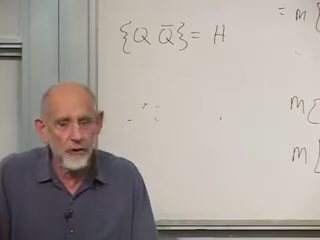
\includegraphics[width=0.62\textwidth]{lecture_05_figure_02.png}
\lectureframe{00:55:46.300}
\caption{黑板上單獨寫出的核心閉合關係。圖中可見花括號和 \(Q,\bar Q,H\)；逗號則依標準反對易子記法補出。}
\end{figure}

能量的加法零點選定為使真空態滿足 \(H=0\)。對超對稱振子而言，這是自然的約定：玻色與費米的零點能貢獻會互相抵消。\editorialnote{講義直接使用總靜止能量，沒有分別列出零點能項；這項約定明確說明了所採用的選擇。}

哈密頓量是偶的，也是一個對稱性生成元：它生成時間平移。因此，若不將偶的時間平移生成元納入，奇生成元就無法彼此閉合。

\begin{classroomqa}
\audiencequestion{這個關係式中哪一項是偶的？是哈密頓量嗎？\lecturetimestamp{00:58:24}}
\lecturerresponse{是。能量是普通的可觀測量，所以 \(H\) 是偶的。超荷 \(Q\) 是奇的，而兩個奇量的乘積是偶的，因此 \(\{Q,\bar Q\}\) 可以等於 \(H\)。奇生成元與偶生成元之間的關係由對易子表示，而不是反對易子。}
\end{classroomqa}

\subsection{補全代數}

同奇偶性的關係式很直接：
\begin{equation}
\{Q,Q\}=2Q^2=0,
\qquad
\{\bar Q,\bar Q\}=2\bar Q^2=0,
\end{equation}
因為 \(Q^2\) 含有 \(c_-^2\)，而 \(\bar Q^2\) 含有 \(c_+^2\)。

接下來要找出它與 \(H\) 的關係。令
\begin{equation}
H\ket{E}=E\ket{E}.
\end{equation}
若玻色子與費米子的質量相等，\(Q\) 會將其中一者轉換為另一者，而不改變能量。因此，\(Q\ket{E}\) 不是零，就是另一個具有相同本徵值的本徵態：
\begin{equation}
H Q\ket{E}=E Q\ket{E}.
\end{equation}
另一方面，
\begin{equation}
QH\ket{E}=Q(E\ket{E})=E Q\ket{E}.
\end{equation}
兩式相減，得到
\begin{equation}
[H,Q]\ket{E}=0.
\end{equation}
若能量本徵態構成完備基底，便可將此結果提升為算符恆等式：
\begin{equation}
[H,Q]=0,
\qquad
[H,\bar Q]=0.
\end{equation}

\begin{classroomqa}
\audiencequestion{如果玻色子與費米子的質量不相同，會發生什麼事？\lecturetimestamp{01:01:16}}
\lecturerresponse{這時將一者轉換成另一者會改變能量，因此所定義的超荷不會與哈密頓量對易，簡單的超對稱性便不成立。對於
\[
H=m_BN_B+m_FN_F,
\]
直接計算可得
\[
[H,Q]=(m_B-m_F)Q.
\]
此式恰在 \(m_B=m_F\) 時為零。\editorialnote{不等質量時的對易子，直接以算符形式表達了能量改變的論證，也明確顯示質量相等的條件。}}
\end{classroomqa}

\begin{classroomqa}
\audiencequestion{能不能更仔細地說明能量本徵態的論證？\lecturetimestamp{01:01:37}}
\lecturerresponse{先從 \(H\ket{E}=E\ket{E}\) 開始。質量相等表示 \(Q\ket{E}\) 具有確定能量 \(E\)，所以 \(HQ\ket{E}=EQ\ket{E}\)。改變運算順序則得到 \(QH\ket{E}=QE\ket{E}=EQ\ket{E}\)，因為 \(E\) 是普通純量。兩者相減後，在每個能量本徵態上都為零。利用本徵態的完備性，就能將這個結論提升為算符方程 \([H,Q]=0\)。}
\end{classroomqa}

因此，完整的玩具模型代數為
\begin{align}
\{Q,\bar Q\}&=H,\\
\{Q,Q\}&=\{\bar Q,\bar Q\}=0,\\
[H,Q]&=[H,\bar Q]=0.
\end{align}
超荷是守恆的奇荷。更令人驚訝的是，它們的代數把改變粒子種類的運算，與時空平移的生成元連結起來。

\section{哈密頓量為何代表時間平移}

這個簡化模型沒有空間座標，但有時間。薛丁格方程為
\begin{equation}
i\frac{\partial}{\partial t}\ket{\psi(t)}
=H\ket{\psi(t)}.
\end{equation}

\begin{figure}[H]
\centering
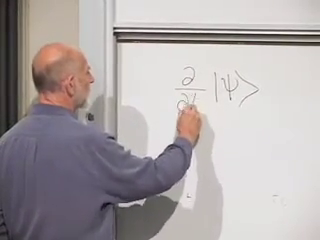
\includegraphics[width=0.56\textwidth]{lecture_05_figure_03.png}
\lectureframe{01:07:26.300}
\caption{時間導數寫在 \(\ket{\psi}\) 旁邊。手遮住了分母的一部分；完整的薛丁格方程已列於上方。}
\end{figure}

對於有限的時間位移 \(\delta\)，
\begin{equation}
\ket{\psi(t+\delta)}
=e^{-iH\delta}\ket{\psi(t)}.
\end{equation}
展開至一階，得
\begin{equation}
\ket{\psi(t+\delta)}
=\left(\mathbf 1-i\delta H\right)\ket{\psi(t)}
+O(\delta^2).
\end{equation}
因此，\(H\) 是使態隨時間演化的無窮小生成元。

同位旋和色等內部對稱性也會改變粒子標記。同位旋可以混合質子態與中子態；色旋轉則混合紅、綠、藍夸克。然而，這些內部變換無論如何組合，都不會使系統在空間或時間中平移。超對稱則不同：
\begin{equation}
\begin{gathered}
\text{odd particle-changing transformation}\\
\mathrel{\stackrel{\{\ ,\ \}}{\Longrightarrow}}\\
\text{time translation}
\end{gathered}
\end{equation}
這提示我們，奇生成元本身可能就是平移，只是平移方向不同於通常的方向。

\section{超空間}

\subsection{時間與奇座標的函數}

引入函數
\begin{equation}
\Psi=\Psi(\theta,\bar\theta,t).
\end{equation}
在玩具模型中，它可以視為波函數；更一般地說，則可視為超場。由於對奇變數的展開會終止，
\begin{equation}
\Psi(\theta,\bar\theta,t)
=A(t)+\bar\chi(t)\theta
+\bar\theta\chi(t)+F(t)\bar\theta\theta.
\end{equation}
單一物件便包含了偶分量函數與奇分量函數。\editorialnote{這個分量展開運用了前面介紹的格拉斯曼多項式，明確呈現了玩具超空間上函數的標準形式。}

普通的時間平移會使 \(\theta,\bar\theta\) 保持不變，並令
\begin{equation}
t\longmapsto t+\delta.
\end{equation}
展開至一階，得
\begin{equation}
\Psi(\theta,\bar\theta,t+\delta)
=\Psi(\theta,\bar\theta,t)
+\delta\,\partial_t\Psi(\theta,\bar\theta,t).
\end{equation}

\begin{figure}[H]
\centering
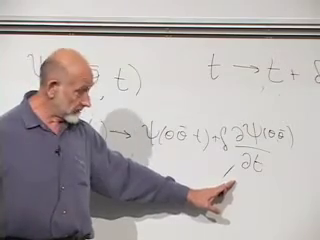
\includegraphics[width=0.72\textwidth]{lecture_05_figure_04.png}
\lectureframe{01:13:15.060}
\caption{黑板上在 \(t\to t+\delta\) 上方寫出 \(\Psi\) 的一階變化，並直接標示其導數項。}
\end{figure}

\subsection{沿奇方向平移}

現在定義一個平移奇座標的變換：
\begin{equation}
\theta\longmapsto\theta+\epsilon,
\end{equation}
其中 \(\epsilon\) 是另一個奇的格拉斯曼參數。同時，讓時間產生一個偶的冪零位移：
\begin{equation}
t\longmapsto t+i\bar\theta\epsilon.
\end{equation}
\(\bar\theta\) 和 \(\epsilon\) 都是奇的，因此兩者的乘積為偶，可以一致地加到偶座標 \(t\) 上。

將參數移到左側後，
\begin{equation}
i\bar\theta\epsilon=-i\epsilon\bar\theta.
\end{equation}
因此誘發的變化為
\begin{align}
\delta_\epsilon\Psi
&=\epsilon\,\partial_\theta\Psi
-i\epsilon\bar\theta\,\partial_t\Psi\\
&=\epsilon q_0\Psi,
\end{align}
其中
\begin{equation}
q_0=\partial_\theta-i\bar\theta\partial_t.
\end{equation}
這個奇微分算符生成上述組合平移。使用左導數時，與之相容的共軛生成元為
\begin{equation}
\bar q_0=-\partial_{\bar\theta}
+i\theta\partial_t.
\end{equation}

具體的符號取決於使用左格拉斯曼導數或右格拉斯曼導數，以及共軛運算如何反轉奇因子的順序。無論採用哪種約定，代數都必須閉合於時間平移。依照上述定義，
\begin{align}
\{q_0,\bar q_0\}
&=i\{\partial_\theta,\theta\}\partial_t
+i\{\bar\theta,\partial_{\bar\theta}\}\partial_t\\
&=2i\partial_t.
\end{align}
導數與導數的乘積項會消失，奇座標的二次項也會消失。兩個混合項各自貢獻 \(i\partial_t\)。

由於薛丁格繪景中的態滿足 \(H=i\partial_t\)，
\begin{equation}
\{q_0,\bar q_0\}=2H.
\end{equation}
若作如下歸一化：
\begin{equation}
q=\frac{q_0}{\sqrt2},
\qquad
\bar q=\frac{\bar q_0}{\sqrt2},
\end{equation}
則
\begin{equation}
\boxed{\{q,\bar q\}=H.}
\end{equation}
\editorialnote{講義刻意逐步處理不確定的符號，最後注意到多出一個因子 2。這裡展示的左導數約定保留了課堂上的計算過程，同時採用一種自洽的歸一化。其他標準約定會將符號的差異分配到座標平移與生成元之中。}

\begin{classroomqa}
\audiencequestion{超空間反對易子最後的因子 2 從何而來？\lecturetimestamp{01:24:21}}
\lecturerresponse{這裡有兩個相等的混合項。一項來自 \(\{\partial_\theta,\theta\}=1\)，另一項來自 \(\{\partial_{\bar\theta},\bar\theta\}=1\)；兩者都乘上時間導數。因此，未歸一化的生成元給出 \(2i\partial_t\)；在每個超荷中乘上因子 \(1/\sqrt2\)，就能恢復先前採用的歸一化。}
\end{classroomqa}

\begin{classroomqa}
\audiencequestion{這個構造是否假設 \(\epsilon\) 很小？\lecturetimestamp{01:24:51}}
\lecturerresponse{這裡用到的是冪零性，而不是普通數值意義上的大小。由於 \(\epsilon^2=0\)，以單一 \(\epsilon\) 展開時，所有項都會在一階後終止。稱它為無窮小或很小，是有用的類比，但截斷是精確的。}
\end{classroomqa}

\editorialnote{格拉斯曼參數沒有普通數值所具有的正大小。它之所以扮演無窮小參數的角色，是因為它具有冪零性，且展開會精確終止。}

\subsection{幾何意義}

這個代數現在有兩種等價的實現方式。在振子圖像中，\(Q\) 和 \(\bar Q\) 會分別將費米子轉換為玻色子、將玻色子轉換為費米子。在幾何圖像中，\(q\) 和 \(\bar q\) 沿奇方向平移函數，同時誘發普通的時間平移。在這兩種圖像中，
\begin{equation}
\begin{gathered}
\{\text{supercharge},\text{conjugate supercharge}\}\\
=\text{time-translation generator}.
\end{gathered}
\end{equation}

包含 \(t,\theta,\bar\theta\) 的廣義座標空間稱為超空間。在相對論性場論中，超空間還包含普通空間座標，而超荷閉合於完整的時空動量 \(P_\mu\)，不只閉合於 \(H=P_0\)。將這種結構彎曲，便會走向超引力。

格拉斯曼變數一方面是有效整理玻色子與費米子計算的工具；另一方面，閉合關係也揭示了更深一層的意義：粒子種類與時空幾何之間的區分不再是絕對的。沿奇方向平移兩次，會產生沿普通方向的位移。自然界是否在實驗上實現了這種結構，是另一個問題；在數學上，這套結構自洽、簡潔，而且具有驚人的剛性。

\chapter{超對稱性為何可能重要}

\lectureoverview{真空漲落串連起本章的各個主題。邊界條件產生卡西米爾力，圈效應威脅希格斯質量，新的虛粒子會改變規範耦合的跑動，而真空能則支配宇宙膨脹。這些問題促使人們考慮低能超對稱性，藉此穩定希格斯標度、提供暗物質候選者，並改善規範耦合的統一。接著，我們以格拉斯曼座標構造超場，並利用貝雷津積分抽取超對稱作用量。}

\section{反射板之間的真空漲落}

我們回到超對稱性，先釐清一個關於卡西米爾效應的問題。將兩塊平行的反射板相隔\(d\)放置。即使沒有任何實粒子，量子場仍有真空漲落。我們可以將它們想像成虛過程，或等價地，視為場的各振子模態的零點運動。板施加了邊界條件，因此板間允許的漲落不同於不受限制空間中的漲落。

重要的不是能量的絕對零點，而是間距改變時所產生的變化。以\(\mathcal E(d)=E(d)/A\)表示單位面積的真空能。一旦\(\mathcal E\)依賴於\(d\)，它便是位能，而單位面積所受的力為
\begin{equation}
\frac{F}{A}=-\frac{d\mathcal E}{dd}.
\end{equation}
因此，虛過程的重新排列會形成可觀測的力。以理想導體板為例，在熟悉的電磁學情況下，能量和壓力為
\begin{align}
\mathcal E(d)&=-\frac{\pi^2}{720\,d^3},\\
\frac{F}{A}&=-\frac{\pi^2}{240\,d^4},
\end{align}
單位為\(\hbar=c=1\)。\editorialnote{這些係數，以及能量每單位面積的\(d^{-3}\)與壓力的\(d^{-4}\)之間的區別，釐清了黑板上提出的量綱問題。這些是理想平行板的標準結果，並非本文在此推導所得。}負號表示吸引力。

\begin{classroomqa}
\audiencequestion{四次方描述的是力還是能量？ \lecturetimestamp{00:04:39}}
\lecturerresponse{在四維時空中的平行板情況下，單位面積的能量按\(d^{-3}\)衰減；對\(d\)微分後，單位面積的力則按\(d^{-4}\)衰減。恢復\(\hbar\)和\(c\)後，量綱分析便可確定這些冪次。}
\end{classroomqa}

有時人們會把這項計算概括為：平行板中斷了虛光子圈。只要不把這種圖像理解得太字面，它便有所助益。精確的計算考察的是允許的場模態頻譜如何改變，或等價地，量子有效作用量如何改變。無論採用哪種說法，都會得到相同的、隨間距改變的能量。

\begin{classroomqa}
\audiencequestion{卡西米爾力可能是排斥力，而非吸引力嗎？ \lecturetimestamp{00:07:48}}
\lecturerresponse{可能。力的正負號並非普遍固定，而是取決於場、幾何形狀、材料和邊界條件。費米子圈效應的圈符號往往與玻色子圈效應相反，這促成了黑板上提出的猜想；然而，單憑費米子統計，並不能普遍推出每個卡西米爾力都必定是排斥力。\editorialnote{這項限定以一般性的陳述取代了課堂上刻意保留試探性的回答，以免造成錯誤的普遍印象。}}
\end{classroomqa}

\subsection{什麼可以作為真空能的證據？}

卡西米爾力已經測得，原子的可觀測量也會受到真空圈效應影響。然而，這兩項事實本身都不能證明絕對真空能會產生引力。卡西米爾實驗測量的是邊界造成的能量差；描述同一個力時，無須賦予無界的絕對零點能總和任何可操作的意義。

決定性的檢驗來自引力。能量就是引力荷。如果空間真空帶有均勻的能量密度，它就必須進入愛因斯坦方程，並影響宇宙膨脹。因此，宇宙加速膨脹便是真空樣成分直接的引力證據。

\begin{classroomqa}
\audiencequestion{為什麼通俗介紹會把真空能說成很神秘，彷彿物理學家不知道它是什麼？ \lecturetimestamp{00:08:19}}
\lecturerresponse{量子場論指出，每個場都有零點貢獻，因此真空能的可能性並不神秘。真正令人困惑的是其數值：為什麼它的引力效應遠小於根據已知量子場和高能截斷所作的估計？令人驚訝的是它幾乎不存在，而不是它本身存在。}
\end{classroomqa}

多年來，觀測上限小得驚人，人們很容易在心理上傾向於將宇宙學常數精確設為零，並尋找能強制相消的原理。然而，改進後的宇宙學觀測發現它有一個很小但非零的值。這項發現並未使真空能在概念上變得陌生，卻讓其受抑制的程度之高變得無法忽視。具體比較取決於所假設的紫外標度，但每一種自然的高能估計都需要巨大的相消。

\section{單一超荷對多粒子態的作用}

在列舉支持超對稱性的理由之前，我們應先釐清一個可能的悖論。玻色子可以任意大量地佔據同一個模態，而費米子模態的佔據數只能是零或一。如果某種對稱性能互換玻色子與費米子，它會不會把同一模態中的一千個玻色子變成一千個受泡利不相容原理禁止的費米子？

不會。費米子生成元一次只改變一個量子。在振子模型中，令\(a\)湮滅一個玻色子，並令\(c^\dagger\)產生其費米子夥伴。一個超荷可以表示為
\begin{equation}
Q=c^\dagger a.
\end{equation}
作用在含有\(n\)個玻色子且不含費米子的態上時，
\begin{equation}
Q\ket{n,0}
=\sqrt n\,\ket{n-1,1}.
\end{equation}
一個玻色子被移除，一個費米子則被加入。再以同一個荷作用一次，結果為零：
\begin{equation}
Q^2=(c^\dagger)^2a^2=0.
\end{equation}
這就是從費米子產生算符繼承而來的冪零性。

\begin{classroomqa}
\audiencequestion{如果許多玻色子佔據同一個態，為什麼超對稱變換不會在該態中產生許多費米子，進而違反泡利不相容原理？ \lecturetimestamp{00:12:05}}
\lecturerresponse{生成元不會取代整個佔據態，而是使態的費米子數改變一個單位。同一個費米子荷不能像普通轉動生成元那樣反覆作用，因為它的平方為零。另一個互補的荷可以反轉這次互換，而兩者的混合反對易子則閉合於時間平移。}
\end{classroomqa}

最後一句至關重要。簡寫\(Q^2=0\)適用於單一手徵分量，或適用於剛才寫出的簡單荷；這並不表示超荷的每一種乘積都為零。在四維超對稱中，
\begin{equation}
\{Q_\alpha,\bar Q_{\dot\beta}\}
=2\sigma^\mu_{\alpha\dot\beta}P_\mu,
\end{equation}
而
\begin{equation}
\{Q_\alpha,Q_\beta\}=0,
\qquad
\{\bar Q_{\dot\alpha},\bar Q_{\dot\beta}\}=0
\end{equation}
則適用於沒有中心荷的最小代數。\editorialnote{這種分量形式精確地說明了課堂上的簡寫：同一個\(Q\)反覆作用會得到零，而超荷與其共軛的反對易子則生成平移。}

\section{考慮低能超對稱性的三個理由}

\begin{classroomqa}
\audiencequestion{除了相消真空能之外，還有其他支持超對稱性的動機嗎？ \lecturetimestamp{00:15:06}}
\lecturerresponse{有三個密切相關的動機：控制希格斯自能、可能存在穩定的暗物質粒子，以及規範耦合在高能下更精確地會合。這些動機都不能證明自然界實現了超對稱性，但合在一起，使超對稱性成為值得認真檢驗的理論。}
\end{classroomqa}

「\emph{低能超對稱性}」是相對而言的說法。這不表示超伴粒子在日常尺度下很輕，而是表示它們的質量沒有遠高於電弱尺度和加速器尺度。如果超伴粒子的質量被推得任意高，這三項論證都會減弱。

\subsection{保護希格斯尺度}

標量質量對高能物理特別敏感。示意而言，玻色子圈圖會產生如下形式的修正
\begin{equation}
\delta m_H^2\big|_{\mathrm B}
\sim +\frac{\lambda}{16\pi^2}\Lambda^2,
\end{equation}
其中\(\Lambda\)表示有效理論適用的能標。費米子圈圖則帶有相反的符號，
\begin{equation}
\delta m_H^2\big|_{\mathrm F}
\sim -\frac{|y|^2}{8\pi^2}\Lambda^2.
\end{equation}
係數取決於相互作用和場的多重度，但超對稱性會將它們聯繫起來，使夥伴粒子之間的主導紫外敏感性相消。\editorialnote{這些示意性的圈圖公式呈現了定性自能論證背後的數學關係，並非完整的標準模型希格斯質量計算。}

這一點很重要，因為希格斯場的真空期望值決定了電弱尺度。規範玻色子和費米子的質量遵循例如下列關係：
\begin{equation}
m_W=\frac{gv}{2},
\qquad
m_f=\frac{y_fv}{\sqrt2}.
\end{equation}
如果希格斯部門自然地被推向極高尺度，除非以極高的精確度調整裸參數來抵消輻射修正，否則我們熟悉的低能粒子譜就會消失。

精確超對稱會使相消完全成立，但觀測到的玻色子與費米子質量不相等，已排除精確超對稱。在軟破缺的超對稱理論中，二次敏感性轉為依賴超伴粒子的質量劈裂，示意而言：
\begin{equation}
\delta m_H^2
\sim
\frac{g^2}{16\pi^2}
\left(m_{\mathrm{soft}}^2-m_{\mathrm{ordinary}}^2\right)
\ln\frac{\Lambda^2}{m_{\mathrm{soft}}^2}.
\end{equation}
只有當劈裂不太大時，這種相消才仍然有用。

\subsection{暗物質級聯的穩定終點}

將粒子譜分成普通粒子及其超伴粒子。費米子有玻色子夥伴，玻色子則有費米子夥伴。如果相互作用保有一種區分這兩類粒子的宇稱，那麼超伴粒子衰變後必須留下另一個超伴粒子：
\begin{equation}
\widetilde X
\longrightarrow X+\widetilde Y
\longrightarrow X+Y+\widetilde Z
\longrightarrow\cdots.
\end{equation}
級聯衰變無法除去最後一個超伴粒子，因此最終會停在最輕超對稱粒子（LSP）。

常用的對稱性是\(R\)宇稱，
\begin{equation}
R_p=(-1)^{3(B-L)+2s}.
\end{equation}
標準模型粒子的\(R_p=+1\)，而其超伴粒子的\(R_p=-1\)。如果\(R_p\)是精確的，每個相互作用都會包含偶數個超伴粒子，LSP也就穩定。\editorialnote{超對稱性本身並不保證LSP穩定。穩定性需要守恆的\(R\)宇稱，或具有相同結果的其他對稱性；若沒有這種對稱性，LSP便可能衰變。}

暗物質必須至少存活一個宇宙學時間尺度。它還必須以足夠弱的方式相互作用，才能反覆穿過可見星系盤，而不損失大量能量。帶電或強作用的粒子群會發生散射、耗散能量，並傾向於像普通物質一樣塌縮至同一個薄盤結構。觀測到的延展暈則指向中性、弱作用的成分。

這無法唯一確定LSP。依模型和對稱性破缺的形式而定，候選者可能是電弱規範費米子與希格斯微子的中性混合態，也可能是引力微子。帶電或帶色荷的候選者受到嚴格限制。超對稱性提供的不是必然的答案，而是一種自然的機制，能產生中性且長壽的終點粒子。

\section{跑動耦合與統一的線索}

第三個動機從電荷屏蔽談起。測得的耦合會隨能量尺度改變，因為虛粒子會修飾相互作用。以電磁作用為例，插入光子傳播子中的電子—正電子圈會在長距離下屏蔽電荷。在更短距離，或更高的動量轉移下，探針之間的極化雲較少，因此有效電荷較大。

寫成
\begin{equation}
\alpha_i=\frac{g_i^2}{4\pi}.
\end{equation}
在一圈近似下，逆耦合會隨能量的對數線性跑動：
\begin{equation}
\frac{d\alpha_i^{-1}}{d\ln\mu}
=-\frac{b_i}{2\pi}.
\end{equation}
因此
\begin{equation}
\alpha_i^{-1}(\mu)
=\alpha_i^{-1}(\mu_0)
-\frac{b_i}{2\pi}\ln\frac{\mu}{\mu_0}.
\end{equation}
\editorialnote{這個一圈方程精確表達了以對數能量為橫軸所畫出的近似直線。閾值效應和高圈修正會使這些線略微彎曲。}

在電弱尺度以上，三個基本規範耦合分別屬於
\begin{equation}
U(1)_Y,\qquad SU(2)_L,\qquad SU(3)_c.
\end{equation}
這三個規範群。低能時用來建立直觀圖像的電磁耦合，是電弱對稱性破缺後前兩個耦合的組合。對量子色動力學（QCD）而言，非阿貝爾規範場會造成反屏蔽：強耦合在短距離下減弱，這就是漸近自由。因此，\(\alpha_3^{-1}\)會隨\(\ln\mu\)增加，而其他逆耦合的斜率則不同。

標準模型的曲線似乎朝彼此靠近，但不會在同一點相交。超伴粒子會改變虛圈效應，因而改變係數\(b_i\)。採用傳統的大統一理論歸一化時，
\begin{align}
(b_1,b_2,b_3)_{\mathrm{SM}}
&=\left(\frac{41}{10},-\frac{19}{6},-7\right),\\
(b_1,b_2,b_3)_{\mathrm{MSSM}}
&=\left(\frac{33}{5},1,-3\right).
\end{align}
若超伴粒子閾值接近 TeV 尺度，外推的超對稱曲線會在
\begin{equation}
M_{\mathrm{GUT}}\sim 10^{16}\ \mathrm{GeV}.
\end{equation}
附近更精確地會合。沒有任何實驗能直接達到該尺度。我們測量低能耦合，由場的內容決定跑動，再將曲線外推許多個數量級。兩條線總會在某處相交；三條彼此獨立的線在同一點附近會合，才是非平凡的觀察。

\begin{classroomqa}
\audiencequestion{改進後的外推是否假設超對稱性精確成立，且超伴粒子質量彼此相等？ \lecturetimestamp{00:38:09}}
\lecturerresponse{不是。超對稱性已破缺，因此粒子質量有所劈裂。關鍵在於超伴粒子的圈效應何時開始影響跑動。如果超伴粒子不太重，斜率會提早改變，讓三個耦合趨於會合。如果它們重得驚人，超對稱閾值便太晚才出現，改進後的會合也就不復存在。}
\end{classroomqa}

閾值修正和未知的高能粒子譜，使我們不能照字面宣稱三條線在數學上精確相交。即便如此，結果仍然相當顯著：同一個有助於穩定希格斯尺度、並提供熱暗物質候選者的近似超伴粒子尺度，也改善了規範耦合的統一。

\subsection{引力與共同的高能尺度}

引力的表現不同，因為引力荷就是能量本身。在質心能量\(E\)下，一個有用的無量綱量度為
\begin{equation}
\alpha_G(E)\sim GE^2
=\left(\frac{E}{M_{\mathrm{Pl}}}\right)^2.
\end{equation}
在一般能量下，這個量小得驚人，但會隨\(E\)的平方增加。因此，它的倒數下降得遠比對數跑動的規範耦合逆值快，並在普朗克尺度附近達到約一的量級。

這項比較暗示，所有相互作用可能都受相近的高能尺度支配，但它不像規範耦合統一那樣明確。規範耦合是可重整場論中的無量綱參數；牛頓常數則有量綱，因此若要把引力放到同一張圖上比較，就必須另作約定。

\begin{classroomqa}
\audiencequestion{超伴粒子也參與相同的三種規範相互作用嗎？還是它們代表新的力？ \lecturetimestamp{00:42:35}}
\lecturerresponse{超伴粒子帶有與其夥伴相同的規範量子數。超電子帶有與電子相同的電荷；超夸克則帶有相應夸克的色荷和電弱荷，雖然兩者的自旋和質量不同。因此，超伴粒子的圈效應會修正相同的規範相互作用，而不會引進三種新的力。}
\end{classroomqa}

\begin{classroomqa}
\audiencequestion{如果在大型強子對撞機（LHC）發現一個超伴粒子，是否就能確證超對稱性？ \lecturetimestamp{00:43:27}}
\lecturerresponse{僅憑名稱，一個陌生粒子的發現還不足以證明什麼；但若發現的超伴粒子譜符合自旋、電荷、質量與耦合之間的超對稱關係，就會極具辨識性。超對稱性施加許多彼此關聯的限制，因此詳細的相互作用模式將提供決定性的檢驗。}
\end{classroomqa}

\subsection{尺度不能毫無代價地任意提高}

如果超伴粒子的質量只略高於實驗可及範圍，這三項動機仍都可能成立。如果其質量提高數個數量級，每項論證都會變弱：
\begin{enumerate}
\item 希格斯質量的相消會留下對質量劈裂仍高度敏感的殘餘效應。
\item 傳統的弱尺度熱遺跡不再以預期的尺度產生。
\item 規範耦合跑動的閾值移至更高處，三個耦合也就較不精確地會合。
\end{enumerate}
超對稱性仍可能存在於高得多的尺度，但它將無法再以同樣簡潔的方式解決這些特定的低能問題。某個想法流傳已久，並不代表自然界必定採用它；這只能說明該理論自洽，值得接受決定性的檢驗。

\section{宇宙學能告訴我們哪些暗物質資訊，又有哪些無法得知}

\begin{classroomqa}
\audiencequestion{標準宇宙學能否像核合成限制氫和氦的含量一樣，確定暗物質的總量和每個暗物質粒子的質量？ \lecturetimestamp{00:46:32}}
\lecturerresponse{宇宙學能相當精確地測出暗物質的總質量密度，但單靠密度無法區分粒子質量和數量。同樣的密度可能由少數重粒子構成，也可能由數量極多的極輕粒子構成。要辨認微觀粒子，還需要額外的理論或非引力觀測。}
\end{classroomqa}

兩種大致的可能性說明了這種模糊性。一種是接近電弱或 TeV 尺度的弱作用粒子，能從熱浴中凍結脫離熱平衡。另一個極端則是極輕的玻色子，例如軸子，能形成相干場組態或凝聚態。這兩種發展最充分的機制位於相反的尺度端點附近，並不表示中間的可能性就被排除。

暈的結構本身提供了一項重要限制。暗物質穿過普通物質時幾乎不受摩擦，因此能維持空間上的延展分布，而不會塌縮成發光物質的盤狀結構。旋轉曲線和其他引力現象告訴我們質量確實存在，但單憑這些現象無法得知粒子數量。

\begin{classroomqa}
\audiencequestion{早期宇宙是否可能起初只有超粒子，後來它們再衰變成我們觀測到的粒子？ \lecturetimestamp{00:49:11}}
\lecturerresponse{當溫度遠高於所有相關質量時，快速反應會使各種粒子趨向熱平衡，而不是維持任意的單邊分布。若超伴粒子數量不足，普通粒子的碰撞會產生超伴粒子；超伴粒子的碰撞和衰變則會補充普通粒子。精確的豐度取決於相互作用和自由度，但熱電漿會持續趨向平衡。}
\end{classroomqa}

宇宙冷卻時，有質量的粒子種類會受到波茲曼因子的抑制，並發生湮滅或衰變。當穩定的LSP之相互作用速率慢於宇宙膨脹率時，它便不再跟隨平衡態：
\begin{equation}
\Gamma_{\mathrm{ann}}
\sim n\langle\sigma v\rangle
\lesssim H.
\end{equation}
剩下的粒子形成遺跡豐度。\editorialnote{這個凍結條件以標準的定量判據補足了熱平衡的論述。其他LSP候選者，尤其是耦合極弱的引力微子，可能具有非熱的演化史。}

\begin{classroomqa}
\audiencequestion{LSP是什麼普通粒子的夥伴？它一定完全不與其他粒子相互作用嗎？ \lecturetimestamp{00:51:05}}
\lecturerresponse{這沒有與模型無關的答案。可行的暗物質LSP預期應為電中性且不帶色荷，但不必完全沒有相互作用。它可能是與光子、弱規範玻色子和希格斯場相關的混合態，也可能是引力微子。其確切身分取決於超對稱破缺後的粒子譜。}
\end{classroomqa}

\section{真空圖、自能圖與膨脹}

\begin{classroomqa}
\audiencequestion{希格斯發散和真空能發散有什麼不同？ \lecturetimestamp{00:52:09}}
\lecturerresponse{真空圖沒有外部粒子線；它會改變空間真空的有效作用量，並對真空能有所貢獻。希格斯自能圖有兩條外部希格斯線；它會改變希格斯傳播子，進而改變希格斯質量。兩者都涉及虛漲落，但所回答的是不同問題。}
\end{classroomqa}

我們可以把實粒子想像成插入真空中的雜質。與這個雜質相連的真空漲落會改變它的傳播和質量。卡西米爾板也會改變真空漲落，但原因是宏觀邊界條件。兩者共有的要素，是量子漲落會對置入其中的對象產生響應；不過，各情況下被修正的可觀測量並不相同。

\vspace{-2pt}
\subsection{物質、輻射與真空的稀釋方式各不相同}

令\(a(t)\)為宇宙標度因子，並令
\begin{equation}
H=\frac{\dot a}{a}
\end{equation}
表示哈伯參數。均勻宇宙中的局部應力能量守恆給出
\begin{equation}
\dot\rho+3H(\rho+p)=0.
\end{equation}
若狀態方程為\(p=w\rho\)，積分後可得
\begin{equation}
\rho(a)\propto a^{-3(1+w)}.
\end{equation}
\editorialnote{連續性方程簡潔地推導出粒子計數和波長拉伸這兩種說明背後的關係。}

對冷的非相對論性物質而言，\(p\approx0\)，因此
\begin{equation}
\rho_m\propto a^{-3}.
\end{equation}
固定的共動體積隨\(a^3\)增大，而其中粒子所帶的靜止能量大致不變。

對輻射而言，\(p=\rho/3\)，因此
\begin{equation}
\rho_r\propto a^{-4}.
\end{equation}
數密度的稀釋貢獻了三個冪次；第四個冪次則來自紅移：
\begin{equation}
\lambda\propto a,
\qquad
E_\gamma=\frac{2\pi\hbar c}{\lambda}\propto a^{-1}.
\end{equation}

\begin{classroomqa}
\audiencequestion{如果光子有波函數，推導稀釋定律時，為什麼可以把它當成粒子而非波來描述？ \lecturetimestamp{00:58:21}}
\lecturerresponse{這種區分不影響標度關係。以粒子描述時，共動體積內的粒子數固定，每個量子的能量都按\(a^{-1}\)紅移。以經典波描述時，波長會拉長，場能量也以相同的幅度下降。哪種說法較容易看出膨脹的影響，就可以採用哪種。}
\end{classroomqa}

真空能的狀態方程為\(p_\Lambda=-\rho_\Lambda\)，因此
\begin{equation}
\rho_\Lambda=\text{constant}.
\end{equation}
它不會隨空間膨脹而稀釋。事實上，一個共動區域包含的真空能為
\begin{equation}
E_\Lambda=\rho_\Lambda a^3V_0,
\end{equation}
會隨其物理體積增大。這便引出我們稍後將討論的能量守恆問題。

不同的冪次描繪出宇宙的演化：輻射下降最快，物質下降較慢，真空能則完全不下降。因此，微小的真空能項在早期宇宙可以忽略，到了晚期卻可能占據主導。依據此處討論的粗略數值，目前的能量組成約有\(70\%\)是真空能、\(30\%\)是物質，輻射所占比例則小得多。

\section{幾何等於能量}

愛因斯坦方程的時間—時間分量，將前述標度律轉化為動力學。黑板上的內容從一句口號和一個幾何項開始。

\begin{figure}[H]
\centering
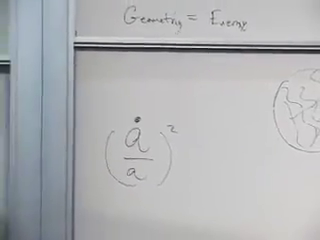
\includegraphics[width=0.68\textwidth]{lecture_06_figure_03.png}
\lectureframe{01:06:37.088}
\caption{黑板上的核心口號是\emph{幾何等於能量}，下方寫著膨脹項\(H^2=(\dot a/a)^2\)。}
\end{figure}

對均勻且各向同性的宇宙，第一條弗里德曼方程為
\begin{equation}
H^2+\frac{k}{a^2}
=\frac{8\pi G}{3}\rho,
\end{equation}
採用\(c=1\)的單位制，其中\(k=+1,0,-1\)表示空間幾何為閉合、平坦或開放，而
\begin{equation}
\rho
=\rho_{\mathrm{ordinary}}
+\rho_{\mathrm{dark}}
+\rho_{\mathrm{radiation}}
+\rho_{\mathrm{vacuum}}.
\end{equation}
\(1/a^2\)旁的正負號，取決於曲率項是留在等式左側，還是移到右側，也取決於\(k\)的取值。

\begin{figure}[H]
\centering
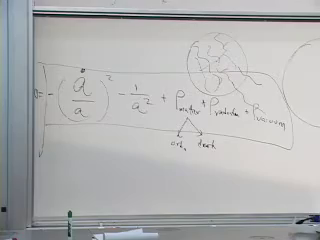
\includegraphics[width=0.96\textwidth]{lecture_06_figure_04.png}
\lectureframe{01:08:46.794}
\caption{完整的黑板平衡式：幾何側包含膨脹和空間曲率，來源側則包含物質、輻射和真空能。物質又分為普通物質與暗物質。}
\end{figure}

\subsection{宇宙學哈密頓約束}

\begin{classroomqa}
\audiencequestion{如果共動區域中的真空能隨宇宙膨脹而增加，那麼是否存在恆定的淨能量密度，或守恆的總能量？ \lecturetimestamp{01:01:51}}
\lecturerresponse{廣義相對論並未為任意膨脹時空提供普遍的全域能量。然而，在均勻宇宙學的約化描述中，愛因斯坦方程的時間—時間分量就是哈密頓約束。將幾何和物質放在同一側時，受約束的哈密頓量為零。變化的物質項由引力自由度來平衡，而非由盒子中某個一般意義上的固定能量來平衡。}
\end{classroomqa}

概略地說，標準表述為
\begin{equation}
\mathcal H_{\mathrm{gravity}}
+\mathcal H_{\mathrm{matter}}
=0.
\end{equation}
「總能量為零」這句話的確切含義就是如此。這是時間重參數化不變性所要求的運動方程，並非聲稱每個局域能量密度都為零。在共動體積中，普通物質的能量大致維持不變，輻射能量則減少，真空能則增加；與此同時，引力貢獻與膨脹率會相應調整，使愛因斯坦約束式持續成立。

局域守恆仍然嚴格成立：
\begin{equation}
\nabla_\mu T^{\mu\nu}=0.
\end{equation}
對均勻流體而言，這正是連續性方程
\(\dot\rho+3H(\rho+p)=0\)。一般而言，失效的是平直時空的直覺：認為在膨脹宇宙中，必定還有一個與座標無關且守恆的物質能量全域總和。\editorialnote{這項區分讓課堂上「能量始終為零」的說法有了精確含義：局域協變守恆與宇宙學哈密頓約束式都嚴格成立，但一般而言，並沒有唯一且定義良好的物質加引力全域能量。}

\begin{classroomqa}
\audiencequestion{零約束式是決定宇宙屬於開放、閉合還是平坦的條件嗎？\lecturetimestamp{01:04:42}}
\lecturerresponse{不是。哈密頓約束式在所有情況下都成立。開放、平坦與閉合宇宙的差異，取決於曲率標記\(k\)，因此也反映在\(k/a^2\)項上。曲率會改變平衡中的一項貢獻，但不會使這項約束式失效或生效。}
\end{classroomqa}

\section{格拉斯曼座標與超場}

\begin{classroomqa}
\audiencequestion{格拉斯曼數真的會出現在理論的拉格朗日量中嗎？\lecturetimestamp{01:09:37}}
\lecturerresponse{它們首先會出現，是因為費米子場是格拉斯曼奇場；其次，它們也作為超空間的座標出現。超場依賴這些奇座標，而超對稱作用量則透過對這些座標求導與積分來構造。}
\end{classroomqa}

普通場是時空的函數，
\begin{equation}
\phi=\phi(x^\mu).
\end{equation}
在四維最小超對稱理論中，\(x^\mu\)會擴充為一個二分量奇旋量\(\theta^\alpha\)及其共軛\(\bar\theta^{\dot\alpha}\)：
\begin{equation}
z^M=(x^\mu,\theta^\alpha,\bar\theta^{\dot\alpha}).
\end{equation}
這裡有兩個複數奇分量，或等價地說，四個實奇方向。超場是定義在這個超空間上的函數：
\begin{equation}
\Phi=\Phi(x,\theta,\bar\theta).
\end{equation}

這些並非度規意義下的微小空間維度。格拉斯曼座標沒有正的數值大小。說它很小，只是幫助理解冪零性的一種說法：
\begin{equation}
(\theta^\alpha)^2=0,
\qquad
\theta^\alpha\theta^\beta=-\theta^\beta\theta^\alpha.
\end{equation}
展開之所以會在有限項後終止，是因為冪零性，而非數值上的微小。\editorialnote{}

有四個獨立奇座標時，一般超場至多包含\(2^4=16\)個格拉斯曼單項式。概略地說，
\begin{equation}
\begin{aligned}
\Phi(x,\Theta)={}&\phi(x)+\Theta_A\psi_A(x)\\
&+\frac{1}{2}\Theta_A\Theta_B Z_{AB}(x)+\cdots\\
&+\Theta_1\Theta_2\Theta_3\Theta_4D(x),
\end{aligned}
\end{equation}
其中\(\Theta_A\)統稱這四個實奇座標。由於整個超場可以取為偶的，偶次項的係數是玻色場，奇次項的係數是費米場。因此，一個超場便能收納由普通分量場組成的有限多重態。

這種收納不只是記號上的便利。超對稱在幾何上表現為奇方向上的平移與時空平移相互混合。依照超空間規則以超場構造的拉格朗日量，會繼承超對稱；這就如同以張量構造的標量拉格朗日量會繼承旋轉或洛倫茲不變性。

作用量現在包含格拉斯曼測度。典型的全超空間項形式如下：
\begin{equation}
S_D=\int d^4x\,d^2\theta\,d^2\bar\theta\,
\mathcal K(\Phi,\Phi^\dagger).
\end{equation}
手徵項則使用以下測度：
\begin{equation}
S_F=\int d^4x\,d^2\theta\,W(\Phi)+\mathrm{h.c.}
\end{equation}
\editorialnote{全超空間測度與手徵測度的區分，是對示意性的\(d^4x\,d^4\theta\)作用量所作的標準細化。要採用哪種測度，得由具體例子來決定。}

因此，我們來到一個普通微積分無法回答的問題：對反交換座標積分，究竟是什麼意思？

\section{貝雷津積分}

\subsection{普通的例子：全導數}

先考慮一個普通函數\(F(x)\)，假設它在\(x\)趨近正、負無窮時都趨近於零。微積分基本定理給出
\begin{equation}
\int_{-\infty}^{\infty}dx\,\frac{dF}{dx}
=F(\infty)-F(-\infty)
=0.
\end{equation}

\begin{figure}[H]
\centering
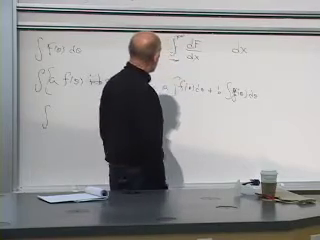
\includegraphics[width=0.88\textwidth]{lecture_06_figure_05.png}
\lectureframe{01:26:31.594}
\caption{這是貝雷津積分的普通原型：全導數的積分可化為端點值；若函數在端點趨近於零，積分便為零。黑板下方的推導有部分被遮住，因此正文列出了完整的方程。}
\end{figure}

我們希望格拉斯曼積分具有線性，並具備全導數積分為零這項實用性質。對單一奇座標，要求
\begin{align}
\int d\theta\,[af(\theta)+bg(\theta)]
&=
a\int d\theta\,f(\theta)
+b\int d\theta\,g(\theta),\\
\int d\theta\,\partial_\theta f(\theta)&=0.
\end{align}
第二個條件是測度平移不變性在代數上的類比。奇數座標軸沒有端點，也不會將它分割成微小區間後逐段求和。

\begin{classroomqa}
\audiencequestion{若沒有不定格拉斯曼積分，是否就得放棄「積分是微分的反運算」這個想法？\lecturetimestamp{01:21:19}}
\lecturerresponse{是的。貝雷津積分是一個定義好的線性泛函，不是求原函數的運算。對單一格拉斯曼變數而言，它實際上可由與微分相同的代數運算表示。}
\end{classroomqa}

\begin{classroomqa}
\audiencequestion{對整個時空的\(d^4x\)積分也是定積分嗎？\lecturetimestamp{01:21:34}}
\lecturerresponse{是的。對作用量在時空上積分時，邊界條件是默認的。兩者的差異在於，普通時空積分可以透過和的極限來理解；格拉斯曼積分則是以代數方式定義，其作用對象是有限基底\(1,\theta\)。}
\end{classroomqa}

\subsection{單一變數}

單一奇變數的任意函數，都可以寫成係數依固定次序置於右側的形式：
\begin{equation}
f(\theta)=a+\theta b.
\end{equation}
由於\(\partial_\theta\theta=1\)，全導數規則意味著
\begin{equation}
\int d\theta\,1=0.
\end{equation}
剩下的歸一化條件取為
\begin{equation}
\int d\theta\,\theta=1.
\end{equation}
因此，
\begin{equation}
\int d\theta\,f(\theta)=b.
\end{equation}
積分會選出最高次項的係數。在此採用左導數約定時，
\begin{equation}
\partial_\theta f=b
=\int d\theta\,f.
\end{equation}

\begin{classroomqa}
\audiencequestion{是否存在一個函數\(F(\theta)\)，使得\(\partial_\theta F=\theta\)？\lecturetimestamp{01:30:05}}
\lecturerresponse{不存在。這樣的函數必須含有一項與\(\theta^2\)成正比，但\(\theta^2=0\)。這也說明了為何格拉斯曼代數中沒有不定積分的類比。}
\end{classroomqa}

\subsection{兩個變數與測度的次序}

對一對複數變數\(\theta,\bar\theta\)，一般偶函數可寫成以下有序形式：
\begin{equation}
f(\theta,\bar\theta)
=a+\bar\theta\psi+\bar\psi\theta+b\,\bar\theta\theta.
\end{equation}
不會有更高次項，因為
\begin{equation}
\theta^2=\bar\theta^2=0,
\qquad
\bar\theta\theta=-\theta\bar\theta.
\end{equation}

現在固定以下約定：
\begin{equation}
\int d\theta\,d\bar\theta\,
\bar\theta\theta=1.
\end{equation}
在迭代積分中，相鄰的\(d\bar\theta\)積分先進行。於是得到下表：
\begin{align}
\int d\theta\,d\bar\theta\,1&=0,\\
\int d\theta\,d\bar\theta\,\theta&=0,\\
\int d\theta\,d\bar\theta\,\bar\theta&=0,\\
\int d\theta\,d\bar\theta\,\bar\theta\theta&=1.
\end{align}
因此，
\begin{equation}
\int d\theta\,d\bar\theta\,
f(\theta,\bar\theta)=b.
\end{equation}

\begin{classroomqa}
\audiencequestion{對於一個與\(\theta\)成正比的項，真的會是對\(\theta\)積分使二重積分歸零嗎？\lecturetimestamp{01:34:59}}
\lecturerresponse{不是；剛才的講解把兩者的作用顛倒了。先對\(\theta\)以\(\theta\)積分，結果為一。積分後的結果不再含有\(\bar\theta\)，而剩下對一的\(\bar\theta\)積分會歸零。無論如何，只有兩個變數都出現時，二重積分才不為零。}
\end{classroomqa}

\begin{classroomqa}
\audiencequestion{若將\(\theta\)與\(\bar\theta\)對調，積分會變號嗎？\lecturetimestamp{01:36:33}}
\lecturerresponse{會。奇變數與奇測度彼此反交換。依照上述約定，
\[
\int d\bar\theta\,d\theta\,\bar\theta\theta=-1.
\]
因此必須選定一種次序並始終一致。物理結果不受約定影響，但中間計算的符號會受影響。}
\end{classroomqa}

對於\(n\)個獨立的格拉斯曼變數，規則一目了然：
\begin{equation}
\int d\theta_n\cdots d\theta_1\,
f(\theta_1,\ldots,\theta_n)
\end{equation}
會取出有序最高次單項式\(\theta_1\cdots\theta_n\)的係數；符號則由所選的變數與測度次序決定。這項簡單的分量提取規則，是構造超空間作用量的關鍵。超對稱變分會成為奇全導數，而超空間積分會將其消去；這就如同普通作用量在適當邊界條件下會消去時空全導數。

\section{如此簡單的微積分為何有如此大的威力}

這些規則看起來幾乎微不足道：
\begin{equation}
\int d\theta\,1=0,
\qquad
\int d\theta\,\theta=1.
\end{equation}
然而，它們讓我們得以構造相互作用場論，並自動維持玻色子與費米子的質量及耦合之間的關係。超空間微積分的目的，與相對論中的張量微積分相同：安排記號，使所需的對稱性在每一項允許的運算下都能維持。

代價是必須仔細處理符號。每交換兩個奇物件，都會多出一個負號；因此，計算在概念上即使正確，也可能因一次次序選擇而出錯。這種困難並非表面問題，而是費米子統計在代數上的映現。

\begin{classroomqa}
\audiencequestion{格拉斯曼數是和超對稱一起發明的嗎？還是更早就已存在？\lecturetimestamp{01:41:19}}
\lecturerresponse{它們早已存在。赫爾曼・格拉斯曼在十九世紀發展出其背後的外代數。微分形式早已使用反交換的基底元素；到了二十世紀，量子場論與超對稱則為同一套數學找到了新的物理角色。}
\end{classroomqa}

現在可以開始進行具體構造了。超場收納完整的玻色子－費米子多重態，超空間導數維持代數結構，貝雷津積分則提取分量作用量。接下來，我們將先在最簡單的一維模型中運用這套方法，再將它應用於場論。

\chapter{超空間與超對稱動力學的構造}

\lectureoverview{我們從超對稱能作用的最小系統出發，重新建構超對稱：一個玻色振子和一個能量相同的費米振子。兩者分別滿足二階和一階方程，這項差異引出超荷及其代數。接著，我們將該代數重新詮釋為座標由普通座標 (t) 和格拉斯曼座標 \(\theta,\bar\theta\) 組成的空間上的幾何。超場將玻色子、費米子和輔助場組合成單一物件；貝列津積分提取出不變的普通拉格朗日量；協變導數使相容於對稱性的約束得以成立；手徵約束則是第一個重要例子。本講刻意呈現這套機制在符號與排序上的難題，最後說明為什麼對稱性本身比費曼規則的彙編更為根本。}

\section{回到單模系統}

讓我們再次從靜止的費米子和玻色子談起。我們省略所有空間座標和動量標記。在給定的模態中，一個量子不是存在就是不存在，只需用創生與湮滅算符便足以描述。以 \(a^\dagger,a\) 表示玻色模態，以 \(c^\dagger,c\) 表示費米模態。它們滿足
\begin{align}
[a,a^\dagger]&=1,
&
\{c,c^\dagger\}&=1,
&
c^2=(c^\dagger)^2&=0.
\end{align}
若兩個量子的能量相同，皆為 \(m\)，那麼除去無關緊要的真空常數後，
\begin{equation}
H=m\left(a^\dagger a+c^\dagger c\right).
\label{eq:l7-one-mode-hamiltonian}
\end{equation}
數目算符 \(a^\dagger a\) 可以取任意非負整數值，而 \(c^\dagger c\) 只能取零或一。這就是這個玩具模型的全部運動學。

這項簡化是策略性的。我們想了解一種操作：在不改變能量的情況下，移除一個玻色子並加入一個費米子，或反過來操作。不過，在建構這種操作之前，我們先把同一個系統從算符語言改寫成拉格朗日量語言。

\section{玻色振子}

對玻色子，引入一個實座標 \(\phi(t)\)。沒有空間變化時，自由標量場就成了一個普通的諧振子。黑板上最初寫下的表示式是
\[
\frac{1}{2}\dot\phi^{,2}+\frac{1}{2}m^2\phi^2.
\]
那是動能加上位能，不是拉格朗日量。講課時立刻修正了符號：
\begin{equation}
L_B=\frac{1}{2}\dot\phi^{,2}-\frac{1}{2}m^2\phi^2.
\label{eq:l7-boson-lagrangian}
\end{equation}

\begin{figure}[H]
\centering
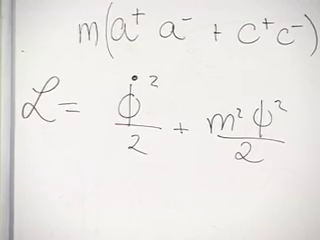
\includegraphics[width=0.62\textwidth]{lecture_07_figure_02.png}
\lectureframe{00:03:25.431}
\caption{位於玻色拉格朗日量上方的單模哈密頓量。畫面保留了口頭修正為 \(T-V\) 之前的初始正號。}
\end{figure}

\begin{classroomqa}
\audiencequestion{所示振子拉格朗日量中的符號有什麼問題？\lecturetimestamp{00:04:00}}
\lecturerresponse{能量是 \(T+V\)，但拉格朗日量是 \(T-V\)。因此，位能項必須帶負號。這項修正使方程從指數變化轉為預期的諧振子振盪。}
\end{classroomqa}

確實，尤拉--拉格朗日方程給出
\begin{align}
\frac{d}{dt}\frac{\partial L_B}{\partial\dot\phi}
&=\frac{\partial L_B}{\partial\phi},\\
\ddot\phi&=-m^2\phi,
\end{align}
也就是
\begin{equation}
\ddot\phi+m^2\phi=0.
\label{eq:l7-boson-eom}
\end{equation}
其頻率是 \(m\)，而不是 \(m^2\)。將這個振子量子化，便會得到與式~\eqref{eq:l7-one-mode-hamiltonian}中由 \(a^\dagger\) 和 \(a\) 描述的相同階梯態。

\section{為什麼費米子作用量是一階的}

費米子拉格朗日量看起來較簡單，因為它只含一個時間導數。從一個刻意簡化的嘗試，已可看出原因。對普通的可交換變數，
\begin{equation}
L_{\mathrm{trial}}=\phi\dot\phi
=\frac{1}{2}\frac{d}{dt}\phi^2.
\end{equation}
這是一個全導數。其尤拉--拉格朗日方程只給出 \(\dot\phi=\dot\phi\)，因此任何可微路徑都符合條件。從作用量中去掉全導數會改變端點資料，但不會改變體內的運動方程。

現在將變數改記為 \(\psi\)，並令它是格拉斯曼奇變數。\(\psi\) 和 \(\dot\psi\) 都會反交換。採用左變分的固定約定時，重新排列奇變數因子會引入負號，因此相同的形式推導得到
\begin{equation}
\frac{d}{dt}\frac{\partial L_{\mathrm{trial}}}{\partial\dot\psi}
=\dot\psi,
\qquad
\frac{\partial L_{\mathrm{trial}}}{\partial\psi}
=-\dot\psi.
\end{equation}
所以方程為
\begin{equation}
\dot\psi=-\dot\psi
\quad\Longrightarrow\quad
\dot\psi=0.
\label{eq:l7-constant-fermion}
\end{equation}
對可交換座標而言只是同義反覆的表示式，對反交換座標卻有了動力學意義。對振子來說，這個方程施加了過多限制，因為它只允許常數解；但這正是我們需要的線索。

\begin{classroomqa}
\audiencequestion{解真的就只是 \(\psi\) 為常數嗎？\lecturetimestamp{00:13:57}}
\lecturerresponse{是的。式~\eqref{eq:l7-constant-fermion} 是一個真正的一階微分方程，其解是任意的格拉斯曼值常數。加入質量項，就能把這個靜態解變成振盪解。}
\end{classroomqa}

顯而易見的嘗試 \(m\psi^2\) 之所以行不通，是因為 \(\psi^2=0\)。我們需要兩個實奇變數 \(\psi_1,\psi_2\)，或者等價地，使用一個複變數及其共軛。講課時在黑板上逐步推導雙實變數形式，並反覆核對符號和因子二。依照慣例正規化的複數形式為
\begin{equation}
L_F=\frac{i}{2}
\left(\bar\psi\dot\psi-\dot{\bar\psi}\psi\right)
-m\bar\psi\psi.
\label{eq:l7-fermion-lagrangian}
\end{equation}
除去一個全導數後，這就是 \(i\bar\psi\dot\psi-m\bar\psi\psi\)。對 \(\bar\psi\) 作變分，得到
\begin{equation}
i\dot\psi=m\psi,
\qquad
\psi(t)=\psi(0)e^{-imt}.
\label{eq:l7-fermion-eom}
\end{equation}
共軛方程的相位則相反。因此，費米子模態也以能量 \(m\) 振盪，與玻色子模態相同，儘管它的方程是一階而非二階。

\editorialnote{~\eqref{eq:l7-fermion-lagrangian} 為探索性的雙實變數計算採用了一種標準排序與正規化。講課時則加入因子 \(i\)、調整一個因子二，並留下某個實分量的符號未定。這些變動不影響核心結論：費米子動力學是一階的，質量以線性形式出現，而複費米子具有非零的雙線性項。}

這是熟悉的相對論性對比在零維情況下的縮影。Klein--Gordon 方程對時間是二階的，而 Dirac 方程是一階的。省略空間後，玻色子是諧振子，費米子則是複數格拉斯曼振子。

\begin{classroomqa}
\audiencequestion{\(\psi\)、\(\dot\psi\)及其共軛的書寫順序重要嗎？\lecturetimestamp{00:18:58}}
\lecturerresponse{中間推導確實會受排序影響，因為奇變數因子會反交換。只要全程採用一致的左變分或右變分、共軛和積分約定，物理理論就不會依賴任意的書寫偏好。交換一對奇變數因子會改變符號，而其他地方也必須一致地調整。}
\end{classroomqa}

結合式~\eqref{eq:l7-boson-lagrangian}和\eqref{eq:l7-fermion-lagrangian}，便能以拉格朗日量描述式~\eqref{eq:l7-one-mode-hamiltonian}所代表的同一組等能配對。現在可以找出它們之間的對稱性了。

\section{超荷及其代數}

移除費米子並加入玻色子的算符為
\begin{equation}
Q^\dagger=\sqrt{2m}\,a^\dagger c,
\end{equation}
其共軛算符則移除玻色子並加入費米子：
\begin{equation}
Q=\sqrt{2m}\,a c^\dagger.
\end{equation}
我們選擇此正規化，使代數具有標準形式。利用 \(cc^\dagger=1-c^\dagger c\)、\(aa^\dagger=a^\dagger a+1\)，以及玻色算符與費米算符彼此可交換這項性質，
\begin{align}
\{Q,Q^\dagger\}
&=2m\left(ac^\dagger a^\dagger c+a^\dagger c a c^\dagger\right)\notag\\
&=2m\left[(a^\dagger a+1)c^\dagger c
+a^\dagger a(1-c^\dagger c)\right]\notag\\
&=2m\left(a^\dagger a+c^\dagger c\right)=2H.
\label{eq:l7-superalgebra}
\end{align}
玻色算符可以移過費米算符。同樣的冪零性限制了費米子的佔據數，並給出
\begin{equation}
Q^2=(Q^\dagger)^2=0.
\end{equation}
最後，
\begin{equation}
[H,Q]=[H,Q^\dagger]=0.
\label{eq:l7-conserved-supercharges}
\end{equation}
每個超荷都以相反方向改變玻色子數和費米子數，因此頻率相同時，兩者造成的能量變化會相消。

\begin{classroomqa}
\audiencequestion{\([H,Q]\) 是什麼？答案會與 \(Q\) 成正比嗎？\lecturetimestamp{00:25:10}}
\lecturerresponse{不，答案是零。單獨的創生或湮滅算符與 \(H\) 對易時，會帶出其能量；但在 \(Q\) 中，玻色子和費米子的貢獻彼此相消。這項相消正是兩者能量相同的結果。}
\end{classroomqa}

\begin{classroomqa}
\audiencequestion{那個對易子不是已經寫在黑板上了嗎？\lecturetimestamp{00:25:45}}
\lecturerresponse{是的。重新推導一次很有用，因為這迫使我們理解這個關係，而不只是照抄：與哈密頓量對易表示該變換是對稱變換，其生成元守恆。}
\end{classroomqa}

「\emph{荷}」一詞反映了這項守恆律。不過，我們不應把 \(Q\) 視為附著在態上的普通數值，也不能把它當成可與其他量同時測量的數值。它是格拉斯曼奇、冪零的算符，會將玻色態映射成費米態。較準確的說法是：它是作用於簡併超多重態中的守恆生成元。
\editorialnote{這樣的措辭修正了課堂上以能量或電荷為態標記的類比。單個非厄米奇超荷不是具有數值量子標記的普通可觀測量。正確的分類依據是它們的守恆作用，以及整個超代數的表示。}

\section{作為導數的生成元}

這個代數很簡潔，但單靠它本身，還無法告訴我們如何建構交互作用理論。下一步是從幾何著手。熟悉的對稱性生成元本來就以微分算符的形式作用。按照講課採用的約定，
\begin{equation}
H=i\frac{\partial}{\partial t},
\qquad
P=-i\frac{\partial}{\partial x}.
\end{equation}

\begin{figure}[H]
\centering
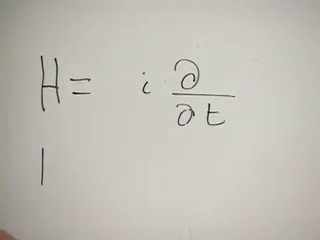
\includegraphics[width=0.50\textwidth]{lecture_07_figure_03.png}
\lectureframe{00:28:12.720}
\caption{哈密頓量表示為時間平移的生成元。}
\end{figure}

角動量同樣是座標與導數的乘積。若超荷是奇生成元，自然會想知道能否用對奇座標微分的方式表示。因此，我們將時間軸擴展為超空間
\begin{equation}
(t,\theta,\bar\theta),
\qquad
\theta^2=\bar\theta^2=0,
\qquad
\theta\bar\theta=-\bar\theta\theta.
\end{equation}
定義在這個空間上的場，依賴普通時間及一對互為共軛的格拉斯曼座標。

本講刻意呈現符號有多容易出錯。複共軛引入的符號、移動奇參數引入的符號，以及選擇左導數而非右導數引入的符號，是三種不同的操作。為避免保留彼此不相容的黑板推導階段，我們現在固定一種約定：所有奇導數都是左導數，並且
\begin{equation}
q=\partial_\theta+i\bar\theta\partial_t,
\qquad
\bar q=\partial_{\bar\theta}+i\theta\partial_t.
\label{eq:l7-differential-supercharges}
\end{equation}
於是
\begin{equation}
q^2=\bar q^{,2}=0,
\qquad
\{q,\bar q\}=2i\partial_t=2H.
\label{eq:l7-differential-algebra}
\end{equation}
因子二來自兩個交叉項：\(\{\partial_\theta,\theta\}=1\)和\(\{\partial_{\bar\theta},\bar\theta\}=1\)。若生成元只含 \(\partial_\theta\) 和 \(\partial_{\bar\theta}\)，它們的反對易子就會是零，無法重現哈密頓量。

\begin{classroomqa}
\audiencequestion{\(q\)和\(\bar q\)中的兩個時間導數項應該帶相同的符號嗎？\lecturetimestamp{00:31:01}}
\lecturerresponse{必須一致選定兩項的符號，才能使混合反對易子等於 \(2H\)。可以採用整體正號的約定，也可以採用與之共軛且始終一致的另一種約定。相對符號應由計算決定，不能憑對符號 \(i\) 的視覺直覺判斷。}
\end{classroomqa}

教室裡一再核對符號，這種困難後來成了笑話：符號好像在通勤上班途中就變了。這個笑話很貼切。讓格拉斯曼參數穿過座標時，反交換可能改變符號，即使物理約定並沒有改變。式~\eqref{eq:l7-differential-supercharges}是後續內容一律採用的固定依據。

\subsection{超對稱性作為座標平移}

令 \(\xi,\bar\xi\) 為無窮小奇參數。按照上述約定，以
\begin{equation}
\delta_\xi=\xi q+\bar\xi\bar q
\end{equation}
作用於超場，等價於施行下列無窮小座標變換：
\begin{align}
\theta&\longrightarrow\theta+\xi,\\
\bar\theta&\longrightarrow\bar\theta+\bar\xi,\\
t&\longrightarrow t+i\left(\xi\bar\theta+\bar\xi\theta\right).
\label{eq:l7-coordinate-shift}
\end{align}
因此，標量超場的變化為
\begin{equation}
\delta_\xi\Phi
=\left(\xi\partial_\theta+\bar\xi\partial_{\bar\theta}
+i\xi\bar\theta\partial_t+i\bar\xi\theta\partial_t\right)\Phi
=\left(\xi q+\bar\xi\bar q\right)\Phi.
\end{equation}
這就是超對稱性的幾何內涵：奇方向上的平移與普通時間平移相連。由於式~\eqref{eq:l7-differential-algebra}，兩個奇平移的合成會閉合為時間平移。

\begin{classroomqa}
\audiencequestion{有爭議的負號是否代表時間向後平移？\lecturetimestamp{00:58:13}}
\lecturerresponse{不同的符號約定可以使寫出的無窮小時間平移方向相反，但這並未引入另一種物理上的逆時過程。關鍵在於，座標變換和微分生成元必須遵守同一個代數。}
\end{classroomqa}

\begin{classroomqa}
\audiencequestion{這種延伸的時間有物理實現嗎？還是只是一種形式上的記帳方式？\lecturetimestamp{00:58:23}}
\lecturerresponse{從一個有用的角度來看，它是一種記帳方式：用幾何形式整理代數。但引入交互作用後，這種整理就有了物理價值。超空間提供系統化的演算，讓我們能逐步建構出保持玻色子--費米子對稱性的拉格朗日量，正如張量演算有助於建構洛倫茲純量。}
\end{classroomqa}

\section{超場與輔助分量}

由於只有兩個奇座標，偶超場的展開會終止：
\begin{equation}
\Phi(t,\theta,\bar\theta)
=\phi(t)+\bar\theta\psi(t)+\bar\psi(t)\theta
+D(t)\bar\theta\theta.
\label{eq:l7-superfield}
\end{equation}
偶單項式 \(\phi\) 和 \(D\) 的係數是玻色量；奇單項式 \(\psi\) 和 \(\bar\psi\) 的係數是費米量。\(\theta^2\)、\(\bar\theta^2\)以及更高次項都不會留下。我們不展開時間依賴，因為對 \(t\) 作普通泰勒展開不會終止，而且在此也沒有必要。

\begin{classroomqa}
\audiencequestion{最高項中的分量 \(D(t)\) 是什麼？\lecturetimestamp{00:41:46}}
\lecturerresponse{此時它只是有限展開中最後一個玻色係數。在分量作用量中，它通常沒有動能項，並透過代數運動方程消去，因此稱為輔助場。本講開玩笑地建議用 ``D 表示 dummy（虛設量），''這點出了它不具動力學的角色，但不是此名稱的歷史由來。}
\end{classroomqa}

超場是單一物件，而 \(\phi,\psi,\bar\psi,D\) 是它的分量。超對稱變換會將這些分量混合。因此，玻色子與費米子的關係，在結構上很像向量的 \(x\) 分量和 \(y\) 分量透過旋轉相互關聯；不過，格拉斯曼方向無法想像成普通的座標軸。

\section{超作用量與最高分量}

要求得運動方程，我們需要作用量。在普通場論中，先構造純量拉格朗日量，再對時空積分。這裡對應的表示式是
\begin{equation}
S=\int dt\,d\theta\,d\bar\theta\;\Lambda
\bigl(\Phi,\text{ superspace derivatives of }\Phi\bigr),
\label{eq:l7-superaction}
\end{equation}
其中 \(\Lambda\) 是偶超場。貝列津積分是代數運算。我們選定
\begin{equation}
\int d\theta\,d\bar\theta\;\bar\theta\theta=1.
\end{equation}
因此，若
\begin{equation}
\Lambda=A+\bar\theta B+\bar B\theta+C\bar\theta\theta,
\end{equation}
則
\begin{equation}
\int d\theta\,d\bar\theta\;\Lambda=C.
\label{eq:l7-top-component}
\end{equation}
對奇座標積分會提取最高分量，留下普通拉格朗日量，再對時間積分。

為什麼結果具有不變性？超對稱變分會平移積分變數。最高分量的變分是時間上的普通全導數，而奇方向的全導數在貝列津積分下為零。在適當的端點條件下，作用量不變。這相當於先建構洛倫茲純量、再對時空積分的超空間版本。

\section{超場的乘積}

從舊超場構造新超場，最簡單的方法就是將它與自身相乘。從式~\eqref{eq:l7-superfield}出發，所有含有 \(\theta^2\) 或 \(\bar\theta^2\) 的項都會消失。維持 \(\bar\theta\theta\) 的排序，並將帶橫線的分量場置於左側，得到
\begin{align}
\Phi^2
={}&\phi^2
+2\phi\bar\theta\psi
+2\phi\bar\psi\theta\notag\\
&+\left(2\phi D-2\bar\psi\psi\right)\bar\theta\theta.
\label{eq:l7-superfield-square}
\end{align}

\begin{figure}[H]
\centering
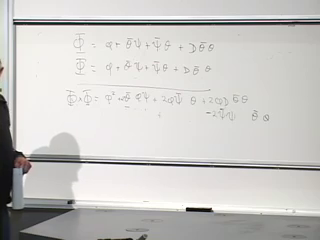
\includegraphics[width=0.82\textwidth]{lecture_07_figure_05.png}
\lectureframe{01:07:57.844}
\caption{逐分量展開的超場乘積，以及其中的 \(\bar\theta\theta\) 項。}
\end{figure}

兩項 \(\phi D\) 和 \(D\phi\) 會相加，因為兩個場都是偶的。兩個費米子交叉項在各自重新排序後也會相加，但共同的符號是負號：
\begin{equation}
(\bar\theta\psi)(\bar\psi\theta)
+(\bar\psi\theta)(\bar\theta\psi)
=-2\bar\psi\psi\,\bar\theta\theta.
\end{equation}
對平方項作奇座標積分，得到
\begin{equation}
\int d\theta\,d\bar\theta\;\Phi^2
=2\phi D-2\bar\psi\psi.
\end{equation}
這一項依照建構方式具有超對稱性，但還不是動能拉格朗日量，因為它不含時間導數。

接著，講者在黑板上提出 \(\Phi^3\)、\(\Phi^4\) 和 \(\Phi^n\) 作為練習，並給出一條簡潔規則。對任意普通函數 \(W\)，
\begin{equation}
\left.W(\Phi)\right|_{\bar\theta\theta}
=W'(\phi)D-W''(\phi)\bar\psi\psi.
\label{eq:l7-function-top-component}
\end{equation}
當 \(W(\phi)=\phi^2\) 時，這會重現式~\eqref{eq:l7-superfield-square}；當 \(W(\phi)=\phi^n\) 時，則得到
\begin{equation}
\left.\Phi^n\right|_{\bar\theta\theta}
=n\phi^{n-1}D-n(n-1)\phi^{n-2}\bar\psi\psi.
\end{equation}
\editorialnote{講者將 \(n\) 次方留作練習，並指出預期會出現哪些類型的項。式~\eqref{eq:l7-function-top-component}則依照固定的排序約定，給出完整規則。}

這時講者問聽眾是否累了。聽眾回答沒有，他則說自己累了。這段對話不只是插科打諢。超場的冪次很容易處理，因為展開會終止；真正棘手的是導數和約束中的符號整理。

\section{哪些導數尊重超對稱性？}

接著討論黑板上的推導之前，先更正一點。普通時間導數沒有問題：
\begin{equation}
[\partial_t,q]=[\partial_t,\bar q]=0.
\end{equation}
因此，只要 \(\Phi\) 是超場，\(\partial_t\Phi\) 也會依照超場的方式變換。較微妙的是裸奇導數 \(\partial_\theta\Phi\) 和 \(\partial_{\bar\theta}\Phi\)，因為它們不會與兩個超荷都反對易。要施加約束並明確地建構超對稱分量，我們需要改造奇導數。
\editorialnote{在此採用的約定下，口頭聲稱時間微分無法產生另一個超場並不正確。由於 \(\partial_t\) 與兩個超荷都對易，它是協變的。後續建構改造後的奇導數仍有必要，這才是本講真正的數學要點。}

\subsection{「``魔法場''」的類比}

講者以普通旋轉說明這項判準。令 \(f(x,y)\) 滿足
\begin{equation}
\partial_y f=0.
\label{eq:l7-magic-constraint}
\end{equation}
稱這類函數為``「魔法場」。''它依賴 \(x\)，但不依賴 \(y\)。魔法場這一類函數在旋轉下是否仍保持？對於
\begin{equation}
L_z=-i\left(x\partial_y-y\partial_x\right),
\end{equation}
我們得到
\begin{equation}
[\partial_y,L_z]=i\partial_x\neq0.
\end{equation}
因此，即使 \(f\) 起初滿足式~\eqref{eq:l7-magic-constraint}，\(L_z f\) 通常仍會產生 \(y\) 依賴性。這項約束並非旋轉不變。

一般原則很簡單。若一個場滿足 \(C\Phi=0\)，而對稱性由 \(G\) 生成，那麼只要 \(C\) 與 \(G\) 的分次對易子為零，變換後的場仍會滿足約束。對兩個奇算符而言，分次對易子就是反對易子。

\begin{classroomqa}
\audiencequestion{場上的約束何時與對稱性相容？\lecturetimestamp{01:17:56}}
\lecturerresponse{當約束算符與對稱性生成元分次對易時。如此一來，\(C(G\Phi)\) 可以將 \(G\) 移到另一側，並化為 \(G(C\Phi)=0\)。旋轉的例子之所以不成立，是因為 \(\partial_y\) 不與旋轉生成元對易。}
\end{classroomqa}

\subsection{協變奇導數}

依照式~\eqref{eq:l7-differential-supercharges}固定超荷後，定義
\begin{equation}
\mathcal D=\partial_\theta-i\bar\theta\partial_t,
\qquad
\bar{\mathcal D}=\partial_{\bar\theta}-i\theta\partial_t.
\label{eq:l7-covariant-derivatives}
\end{equation}
唯一的差異是時間導數項的符號。直接計算得到
\begin{align}
\{\mathcal D,q\}
&=\{\mathcal D,\bar q\}
=\{\bar{\mathcal D},q\}
=\{\bar{\mathcal D},\bar q\}=0,\\
\{\mathcal D,\bar{\mathcal D}\}&=-2i\partial_t.
\label{eq:l7-covariant-algebra}
\end{align}
兩個可能不為零的交叉項會互相抵消。這是奇方向上的協變導數：它在執行微分的同時，保留場的變換規律。

講課時，\(D\)同時用來表示輔助分量和這個導數。我們以\(D(t)\)表示分量，以花體的\(\mathcal D\)表示算符。

\section{手徵約束}

現在可以施加一個在超對稱變換下仍能成立的非平凡約束：
\begin{equation}
\bar{\mathcal D}\Phi=0.
\label{eq:l7-chiral-constraint}
\end{equation}
滿足此條件的場稱為手徵場。若某個場在超對稱變換前是手徵場，則
\begin{equation}
\bar{\mathcal D}(q\Phi)
=-q(\bar{\mathcal D}\Phi)=0,
\qquad
\bar{\mathcal D}(\bar q\Phi)
=-\bar q(\bar{\mathcal D}\Phi)=0.
\end{equation}
因此，變換後的整個超場仍屬於受約束的場類。手徵條件不像魔法場條件，能與此對稱性相容。

為求解此約束，定義平移後的時間座標
\begin{equation}
\tau=t+i\bar\theta\theta.
\label{eq:l7-chiral-time}
\end{equation}
由於我們使用左導數，
\begin{equation}
\partial_{\bar\theta}\tau=i\theta,
\end{equation}
因此
\begin{equation}
\bar{\mathcal D}F(\tau,\theta)
=\left(\partial_{\bar\theta}-i\theta\partial_t\right)F(\tau,\theta)
=i\theta\partial_\tau F-i\theta\partial_\tau F=0.
\end{equation}
一般的局域手徵超場只透過 \(\tau\) 依賴 \(\bar\theta\)：
\begin{equation}
\Phi_{\mathrm{ch}}(\tau,\theta)
=\phi(\tau)+\bar\psi(\tau)\theta.
\label{eq:l7-chiral-field-tau}
\end{equation}

\begin{classroomqa}
\audiencequestion{只有依賴 \(\tau\) 和 \(\theta\) 這種形式，才能滿足手徵約束嗎？\lecturetimestamp{01:32:35}}
\lecturerresponse{局域而言，是的。微分方程 \(\bar{\mathcal D}\Phi=0\) 正表示獨立的 \(\bar\theta\) 依賴可吸收到平移後的座標 \(\tau=t+i\bar\theta\theta\) 中。剩下的有限展開是 \(\tau\) 的函數，再加上一個與 \(\theta\) 成正比的項。}
\end{classroomqa}

改用原來的時間座標重新展開，
\begin{align}
\phi(\tau)
&=\phi(t)+i\bar\theta\theta\dot\phi(t),\\
\bar\psi(\tau)\theta
&=\bar\psi(t)\theta,
\end{align}
因為第二行的修正項含有 \(\theta^2\)。因此，
\begin{equation}
\Phi_{\mathrm{ch}}(t,\theta,\bar\theta)
=\phi(t)+\bar\psi(t)\theta
+i\bar\theta\theta\dot\phi(t).
\label{eq:l7-chiral-field-components}
\end{equation}

\begin{classroomqa}
\audiencequestion{\(\phi(t+i\bar\theta\theta)\)的泰勒展開應該包含二階項嗎？\lecturetimestamp{01:33:51}}
\lecturerresponse{不需要。第一個修正項是 \(i\bar\theta\theta\dot\phi\)，而所有更高階修正項都含有 \((\bar\theta\theta)^2=0\)。聽眾立刻指出這點：冪零性已產生前兩項，並使級數就此終止。}
\end{classroomqa}

這就是手徵性的精簡之處。式~\eqref{eq:l7-superfield}中的未受約束超場有兩個玻色分量槽和兩個費米分量槽。在這個最小的一維例子中，手徵條件移除了獨立的輔助分量槽，並將最高分量與\(\dot\phi\)連結起來。

\section{適時停止的計算}

自然的下一步是將手徵場與其共軛相乘，再對超空間積分。講者開始寫共軛場的展開式時，一位聽眾問，共軛後 \(\theta\bar\theta\) 的順序是否必須反轉。此時符號已經不太可靠。講者沒有勉強作答，而是停下計算。

\begin{classroomqa}
\audiencequestion{即使延後共軛場的乘法，能否先說明關鍵結論？\lecturetimestamp{01:37:30}}
\lecturerresponse{可以。只要一致處理符號與共軛，由手徵場及其共軛構成的超空間表示式，就會產生所需的普通玻色與費米動能項。本講的重要成果是建構原理，而不是從疲憊推導中照抄不可靠的最後一行。}
\end{classroomqa}

應該保留這個停止點。這套形式體系不容出錯：一個奇因子的位置不對，就會改變符號；而共軛、微分、乘法和積分必須始終遵守同一套約定。若無法確保整個推導鏈條一致，正確做法是先修正，再繼續。在標準約定下，熟知的動能作用量由共軛乘積建構而成；但詳細的分量化簡應留待下一次完整推導，不宜從未完成的黑板式子中重建。

\section{為什麼對稱性才是重點}

超對稱拉格朗日量不只是把玻色子和費米子並列而已。它會約束兩者的質量與交互作用，使它們構成超代數的一個表示。在精確超對稱的真空中，同一超多重態的成員具有相同質量。它們的圈圖貢獻彼此關聯，而玻色子與費米子的紫外效應會依照對稱性所要求的精確組合相消。

這就是建構方法重要的原因。我們可以列出費曼頂點，再逐個圖形驗證相消，但如此一來，相消便像是偶然發生。超對稱性說明了這些相消的原因，正如洛倫茲對稱性說明散射振幅為何在所有慣性座標系中都遵循一致的變換規律。

\editorialnote{精確超對稱並不表示每一項個別的自能修正都會消失。它會關聯各種重整化，並消除特定的紫外敏感性；不重整化定理的適用範圍則取決於所討論的物理量、時空維度和超對稱數量。本講關於廣泛相消的說法，應保留這些限定。}

\begin{classroomqa}
\audiencequestion{``chiral''怎麼拼？\lecturetimestamp{01:39:48}}
\lecturerresponse{C-H-I-R-A-L。這個詞描述約束\(\bar{\mathcal D}\Phi=0\)，不是指三維空間物體一般所說的幾何手性；不過，此術語的源頭確實與相對論性旋量的左手和右手結構有關。}
\end{classroomqa}

\begin{classroomqa}
\audiencequestion{能不能跳過拉格朗日量，直接使用超對稱費曼規則？\lecturetimestamp{01:40:00}}
\lecturerresponse{當然可以直接列出規則，但如此一來，耦合之間的關係及其所導致的相消，就會像是無法解釋的巧合。更深層的內涵是廣義的時空對稱性。拉格朗日量或等價的不變形式，能揭示其中原因並有系統地導出這些規則。}
\end{classroomqa}

假設每一個微擾階都碰巧給出洛侖茲不變的振幅，儘管從未提及洛侖茲變換。經過足夠多的計算後，我們會要求一個解釋。答案會是能同時組織所有階的時空對稱性。超空間的作用也類似：\(\theta,\bar\theta\)中的位移會混合玻色與費米分量，而其代數會閉合於時空平移。

\begin{classroomqa}
\audiencequestion{普通空間座標是否也應像格拉斯曼座標一樣，展開成有限冪級數？\lecturetimestamp{01:44:55}}
\lecturerresponse{不會。普通座標的冪級數不會終止，通常也不是自然的分解方式。傅立葉變換更有用，因為它能將場分解成波與動量。對\(\theta\)展開之所以特殊，正是因為冪零性使展開在有限項後終止。}
\end{classroomqa}

\begin{classroomqa}
\audiencequestion{如果大型強子對撞機（LHC）出現一種新粒子，我們要如何判斷它是超伴粒子，而不只是某種未知粒子？\lecturetimestamp{01:45:42}}
\lecturerresponse{超對稱預言的是彼此關聯的量子數與相互作用，而不只是一個額外的粒子態。自旋相差二分之一，規範荷彼此關聯；許多三次與四次耦合所需的獨立參數，也比一般理論少。截面、分支比以及其餘粒子譜都必須符合這些關係。}
\end{classroomqa}

單一個陌生的共振態本身不足以證明超對稱；一整套耦合關係與粒子譜關係才足以構成證據。這正是超空間構造在實驗上的對應：表面上彼此獨立的分量相互作用，都源自同一個不變物件。

\begin{classroomqa}
\audiencequestion{觀測到的粒子與其假想的超對稱伴粒子，質量並不相等。這會如何改變理論？\lecturetimestamp{01:47:01}}
\lecturerresponse{改變極大。超對稱必須破缺，而通常是透過自發破缺，再將破缺效應傳遞到可觀測部門。破缺會使多重態中的粒子質量分裂，同時保留足夠的結構來控制相互作用；若破缺尺度夠低，也能控制紫外修正。釐清這套機制本身就是一項龐大的理論工作，尤其是在納入引力時。}
\end{classroomqa}

\section{原理簡單，計算繁難}

結尾的評述格外坦率。起點聽來很簡單：玻色子與費米子由一種對稱性聯繫起來。然而，實際建構很快就成了處理指標、共軛、格拉斯曼變數排列次序與正負號的學問。即使建構出這種對稱性，現實的粒子物理仍需要讓它破缺；將它與引力耦合則會引向超引力，並增添另一層結構。

這種困難並不代表這個想法空洞。大自然沒有義務讓簡單的原理易於計算。專家透過一再處理細節來學習這門學問，直到符號規則變得熟稔自然。令人挫折之處，在於精簡的代數
\begin{equation}
\{Q,Q^\dagger\}=2H
\end{equation}
與在相互作用理論中實現它所需的大量技術細節之間，存在著一段距離。

\begin{classroomqa}
\audiencequestion{再多一層抽象，最終能簡化形式體系嗎？還是複雜性會不斷累積？\lecturetimestamp{01:49:33}}
\lecturerresponse{目前沒有任何一般性的簡化能免除繁複的細節工作。底層規則或許簡短，但要可靠地運用它們，就必須反覆掌握各種約定。這就是為什麼完整講授這門學問，通常得用上一整門技術課程，而不是廣泛涵蓋粒子物理的課程中的一小部分。}
\end{classroomqa}

\begin{classroomqa}
\audiencequestion{這些變換能告訴我們費米子與玻色子究竟是什麼，或是為什麼它們通常呈現不同的行為嗎？\lecturetimestamp{01:51:42}}
\lecturerresponse{它們告訴我們，兩者是同一個超場的分量，並且在超荷作用下互為映像。作用\(Q\)會將玻色分量映射為費米分量；再進行一次變換，則會產生導數與輔助分量。這類似於旋轉混合向量的各個分量，但不能將它轉化成同樣字面的圖像：適當的描述方式是格拉斯曼幾何本身。}
\end{classroomqa}

這個回答讓我們回到核心思想。超對稱變換是超空間中的微小變換。它會混合\(\phi,\psi,\bar\psi,D\)，如同普通旋轉會混合各個分量；而這些變換的代數會閉合為時間平移。這個圖像雖然抽象，卻並非任意構造：超場中的每一項、協變導數中的每個符號，以及分量相互作用之間的每種關係，都是為了實現這套代數而存在。

\section{我們建構了什麼}

我們從相配的振子哈密頓量出發，並找回它的兩種不同拉格朗日描述。玻色子滿足二階振子方程；費米子則需要一階格拉斯曼作用量，以及一對複數的奇分量。超荷會交換這兩個模式，各自平方為零；它們的反對易子給出哈密頓量，且各自與哈密頓量對易。

將這些荷表示為微分算符，便引出了超空間。有限的超場展開將玻色、費米與輔助分量組合起來；別列津積分選出超拉格朗日量的最高分量；乘法則產生可能的不變相互作用項。接著，為了要求奇導數與對稱性相容，我們引入\(\mathcal D,\bar{\mathcal D}\)、手徵約束，以及位移後的座標\(\tau=t+i\bar\theta\theta\)。

尚未完成的共軛乘積計算，也是這一課的一部分，並非需要掩飾的缺陷。超對稱起源於簡單的物理要求，但其微積分對每一種排列次序都很敏感。掌握這些次序後，便能得到豐厚的成果：對稱性組織了質量與耦合，量子修正滿足並非偶然的關係，而玻色子與費米子則成為同一個幾何物件的分量。

\chapter{四維超對稱與 Wess--Zumino 模型}

\lectureoverview{上一講的一維超對稱代數只涉及哈密頓量。現在，洛侖茲不變性迫使能量重新與空間動量結合，超荷也必須成為二分量旋量。我們先回到無質量 Weyl 費米子及其哈密頓量 \(H=\boldsymbol{\sigma}\cdot\mathbf p\)，由此導出該代數。接著，我們將超荷表示為四維超空間上的微分算符，以約束 \(\bar D_{\dot\alpha}\Phi=0\) 篩選出手徵超場，並利用超空間積分構造具體的場論。依序選取 \(\Phi^\dagger\Phi\)、\(\Phi^2\) 和 \(\Phi^3\)，便會得到傳播、玻色子--費米子質量相等、Yukawa 相互作用，以及相關的標量相互作用。輔助場 \(F\) 使這些關係一目了然；最後的圈圖則說明超對稱為何能減緩紫外敏感性。}

\section{為什麼哈密頓量不能獨立存在}

在玩具模型中，空間座標被省略，基本關係是
\begin{equation}
\{Q,Q^\dagger\}=2H.
\label{eq:l8-time-only-algebra}
\end{equation}
若時間是唯一的座標，這種形式便已足夠。然而在相對論性理論中，\(H=P_0\)是四動量 \(P_\mu\) 的一個分量。洛侖茲推進會使它與 \(P_i\) 混合。若代數右側只特別挑出 \(P_0\)，就不可能以協變的方式變換。

因此，修正必須同時做到兩件事：以四個分量 \(P_\mu\) 取代 \(H\)，並在左側提供能與右側洛侖茲向量相配的指標。無質量 Dirac 方程提供了線索：相對論性費米子可以用二分量旋量描述，而矩陣 \(\sigma^\mu\) 能將向量指標轉換成一對旋量指標。

\section{無質量費米子、螺旋度與手徵性}

先看有質量粒子與無質量粒子之間的物理差異。取一個自旋為 \(\tfrac12\) 的有質量粒子，令它沿著自旋方向運動。由於它的速度小於光速，觀察者可以超越它。在新的參考系中，動量反向而自旋不變，因此螺旋度也反向。所以，洛侖茲不變的有質量理論必須同時包含兩種螺旋度。

沒有觀察者能超越無質量粒子。適當的洛侖茲變換無法使其動量相對於自旋反向，因此一個不可約的無質量表示可以只帶有一種螺旋度。空間旋轉可以轉變粒子的運動方向，卻不會把右手變成左手。

\begin{classroomqa}
\audiencequestion{超越粒子的論證，說的真的是螺旋度而不是手徵性嗎？\lecturetimestamp{00:05:42}}
\lecturerresponse{是的。螺旋度是自旋在動量方向上的投影；手徵性則是手徵矩陣的本徵值，通常記為 \(\gamma^5\)。對無質量模式而言，這兩個標籤彼此相連，所以在這個例子中聽起來像是可以互換。對有質量粒子而言，兩者則有所不同。}
\end{classroomqa}

態數的說法需要加上一項限定。\editorialnote{單一無質量 Weyl 場有一種粒子螺旋度，以及相反的反粒子螺旋度。因此，「態數減半」指的是從四分量 Dirac 場縮減為單一二分量 Weyl 場；這並不表示反粒子態消失了。}

將這段開頭論證所用的 Weyl 場寫成
\begin{equation}
\chi=
\begin{pmatrix}
\chi_1\\
\chi_2
\end{pmatrix},
\end{equation}
本講以 \(\psi_\alpha\) 表示這個場；為了避免與下文通常放在手徵超場中的共軛 Weyl 表示混淆，我們在此將它記為 \(\chi\)。
\begin{equation}
H\chi=\boldsymbol{\sigma}\cdot\mathbf p\,\chi.
\label{eq:l8-weyl-hamiltonian}
\end{equation}
對動量 \(\mathbf p\) 而言，矩陣 \(\boldsymbol{\sigma}\cdot\mathbf p\) 的本徵值為 \(\pm|\mathbf p|\)。正頻支提供粒子模式；負頻支則透過反粒子構造重新詮釋，而不會被保留為能譜無下界的分支。

\begin{figure}[H]
\centering
\includegraphics[width=0.70\textwidth]{lecture_08_figure_02.png}
\lectureframe{00:07:44.271}
\caption{手徵二分量旋量與哈密頓量 \(H=\boldsymbol{\sigma}\cdot\mathbf p\)。末尾的動量符號有一部分被遮住，但口述方程可確定其內容。}
\end{figure}

手徵性標籤也取決於慣例。\editorialnote{黑板上將 \(\boldsymbol{\sigma}\cdot\mathbf p\) 的正本徵值直接對應到一種手性。哪一種手徵性對應這個符號，取決於 \(\sigma^\mu\)、\(\bar\sigma^\mu\) 和 Weyl 場的定義。我們保留本徵值的陳述，但不將它標記為不受慣例影響的左手或右手。}

以 \(i\partial_t\) 取代 \(H\)，並以 \(-i\nabla\) 取代 \(\mathbf p\)，得到
\begin{equation}
i\partial_t\chi=-i\boldsymbol{\sigma}\cdot\nabla\chi.
\end{equation}
再定義
\begin{equation}
\begin{aligned}
\sigma^\mu&=(\mathbf 1,\boldsymbol{\sigma}),\\
\bar\sigma^\mu&=(\mathbf 1,-\boldsymbol{\sigma}),\\
\eta_{\mu\nu}&=\operatorname{diag}(1,-1,-1,-1).
\end{aligned}
\label{eq:l8-sigma-convention}
\end{equation}
於是，剛才得到的方程可寫成
\begin{equation}
i\sigma^\mu\partial_\mu\chi=0.
\label{eq:l8-weyl-equation}
\end{equation}
共軛 Weyl 表示使用 \(\bar\sigma^\mu\)。下文稱為 \(\psi_\alpha\) 的正是這個共軛表示，其自由場方程為 \(i\bar\sigma^\mu\partial_\mu\psi=0\)。要證明協變性，必須使用洛侖茲群的旋量表示；此處重要的是其結構：四個矩陣 \(\sigma^\mu\) 將一個時空指標連接到兩個旋量指標。

\section{四維超代數}

現在，奇座標必須像 Weyl 旋量一樣變換：
\begin{equation}
\theta^\alpha=(\theta^1,\theta^2),
\qquad
\bar\theta^{\dot\alpha}=(\bar\theta^{\dot1},\bar\theta^{\dot2}).
\end{equation}
上橫線表示複共軛；上方的點則用來區分共軛的洛侖茲表示。這裡有兩個複 Grassmann 分量，也就是四個實分量。因此，一般的偶超場
\begin{equation}
\mathcal S=\mathcal S(x^\mu,\theta^\alpha,\bar\theta^{\dot\alpha})
\end{equation}
具有有限的 Grassmann 展開。其最高次單項式是
\begin{equation}
\theta^2\bar\theta^2
\equiv
(\theta^1\theta^2)(\bar\theta^{\dot1}\bar\theta^{\dot2}),
\end{equation}
也就是全部四個獨立奇座標的乘積。這個單項式的係數通常稱為 \(D\) 分量。

超荷也帶有旋量指標。在四維 \(N=1\) 超對稱中，代數為
\begin{align}
\{Q_\alpha,\bar Q_{\dot\beta}\}
&=2\sigma^\mu_{\alpha\dot\beta}P_\mu,
\label{eq:l8-superalgebra-main}\\
\{Q_\alpha,Q_\beta\}&=0,
&
\{\bar Q_{\dot\alpha},\bar Q_{\dot\beta}\}&=0,
\label{eq:l8-superalgebra-nilpotent}\\
[P_\mu,Q_\alpha]&=0,
&
[P_\mu,\bar Q_{\dot\alpha}]&=0,
&
[P_\mu,P_\nu]&=0.
\label{eq:l8-superalgebra-commutators}
\end{align}
因子二是慣例上的選擇。矩陣
\(\sigma^\mu_{\alpha\dot\beta}\)
將向量指標與 \(P_\mu\) 縮併，恰好留下等式左側出現的兩個旋量指標。

\begin{classroomqa}
\audiencequestion{\(\alpha\) 和 \(\beta\) 是 sigma 矩陣的矩陣指標嗎？\lecturetimestamp{00:22:01}}
\lecturerresponse{是的。更精確地說，一個是無點的 Weyl 指標，另一個是有點的共軛指標；\(\mu\) 則是時空向量指標。sigma 矩陣連接了這兩種描述。}
\end{classroomqa}

整理後的記號清楚呈現了這種連接。\editorialnote{講課時刻意省略了有點指標，並在黑板上討論 \(\alpha\beta\) 與 \(\beta\alpha\) 的順序。方程~\eqref{eq:l8-superalgebra-main}和\eqref{eq:l8-superalgebra-commutators}補回標準的有點與無點記號，但不改變原本的論證。}

最後一行表示超荷守恆，且與平移相容。動量分量彼此對易，因為它們以導數表示時也彼此對易。依照下文採用的微分慣例，
\begin{equation}
P_\mu=i\partial_\mu,
\end{equation}
因此，式~\eqref{eq:l8-superalgebra-main}也可以寫成
\begin{equation}
\{Q_\alpha,\bar Q_{\dot\beta}\}
=2i\sigma^\mu_{\alpha\dot\beta}\partial_\mu.
\end{equation}

\section{以超空間導數表示超荷}

動量使一般座標平移；超荷則使奇座標平移，同時也會移動時空。採用左作用的 Grassmann 導數，並定義
\begin{align}
Q_\alpha
&=\partial_\alpha
-i\sigma^\mu_{\alpha\dot\alpha}
\bar\theta^{\dot\alpha}\partial_\mu,
\label{eq:l8-Q}\\
\bar Q_{\dot\alpha}
&=-\bar\partial_{\dot\alpha}
+i\theta^\alpha\sigma^\mu_{\alpha\dot\alpha}\partial_\mu.
\label{eq:l8-Qbar}
\end{align}
以 \(\epsilon^\alpha Q_\alpha+
\bar\epsilon_{\dot\alpha}\bar Q^{\dot\alpha}\) 作用於超場，便得到無窮小超對稱變換。超場的分量就是各個獨立 Grassmann 單項式的係數，而微分算符會使這些係數彼此混合。

\begin{classroomqa}
\audiencequestion{簡寫 \(\bar\theta\sigma\partial\) 中指的是哪個 \(x\) 導數？\lecturetimestamp{00:25:40}}
\lecturerresponse{四個分量全都包括在內。\(\bar\theta^{\dot\alpha}\sigma^\mu_{\alpha\dot\alpha}\partial_\mu\) 中重複出現的 \(\mu\) 表示採用求和約定，因此 \(\sigma^\mu\) 的每個分量都會與相應的導數 \(\partial/\partial x^\mu\) 配對。}
\end{classroomqa}

\begin{classroomqa}
\audiencequestion{共軛超荷中應該包含 \(\theta\)，而不是另一個 \(\bar\theta\)，對嗎？\lecturetimestamp{00:26:16}}
\lecturerresponse{對。\(Q\) 對 \(\theta\) 微分，並包含 \(\bar\theta\)；\(\bar Q\) 對 \(\bar\theta\) 微分，並包含 \(\theta\)。兩者是共軛算符。}
\end{classroomqa}

\begin{classroomqa}
\audiencequestion{\(\sigma^\mu\) 是對稱矩陣嗎？\lecturetimestamp{00:27:04}}
\lecturerresponse{Pauli 矩陣是 Hermite 矩陣。\((\mathbf1,\boldsymbol{\sigma})\) 中的四個矩陣有三個是對稱的，而 \(\sigma^2\) 在一般轉置下是反對稱的。這裡相關的共軛性質是 Hermite 性質，以及有點與無點指標的配置。}
\end{classroomqa}

\begin{classroomqa}
\audiencequestion{共軛方程中的 sigma 矩陣，指標順序是否相反？\lecturetimestamp{00:27:13}}
\lecturerresponse{共軛會交換有點與無點表示，因此穩妥的記法是 \(\sigma^\mu_{\alpha\dot\alpha}\) 及其共軛 \(\bar\sigma^{\mu\,\dot\alpha\alpha}\)，而不是把這兩個標籤視為可以互換的矩陣指標位置。}
\end{classroomqa}

式~\eqref{eq:l8-Q}和\eqref{eq:l8-Qbar}中的公式，在表面符號上與黑板上的簡寫不同。這些符號差異與 \(P_\mu\) 採用 \(+i\partial_\mu\) 或 \(-i\partial_\mu\)、導數從左側或右側作用，以及共軛奇變數的排列方式有關。重要的是，同一套慣例必須能同時滿足整個代數。

\section{在超對稱下保持成立的約束}

一般超場含有許多分量。我們要找出一個較小的場類別，同時不破壞對稱性。講課時先舉一個普通的類比。對向量 \(\mathbf V\) 而言，約束
\begin{equation}
V_x=0
\end{equation}
不是旋轉不變的：旋轉後，\(V_y\)會對新的 \(x\) 分量有所貢獻。相較之下，
\begin{equation}
\mathbf V^2=1
\end{equation}
是旋轉不變的，而且會移除一個獨立自由度。有用的約束必須在對稱變換下，將受約束的場映到仍受約束的場。

假設線性奇算符 \(\bar D_{\dot\alpha}\) 定義了條件
\begin{equation}
\bar D_{\dot\alpha}\Phi=0.
\label{eq:l8-chiral-constraint}
\end{equation}
在超對稱變換 \(\delta\Phi=Q\Phi\) 之後，只要 \(\bar D\) 與超荷反對易，同一條件便仍然成立：
\begin{equation}
\bar D(Q\Phi)=-Q(\bar D\Phi)=0.
\end{equation}
這項抽象的一致性檢驗說明了為何要如此構造，而非毫無解釋地直接給出定義。

\begin{classroomqa}
\audiencequestion{在最後一個式子中，為什麼可以交換 \(Q\) 和 \(\bar D\) 的順序？\lecturetimestamp{00:36:56}}
\lecturerresponse{它們是選定為彼此反對易的奇算符。交換順序因此會產生負號；當 \(\bar D\) 作用到 \(\Phi\) 上時，原先的約束便使結果為零。}
\end{classroomqa}

所需的協變導數，只要將其中時空導數項的符號相對於超荷反轉，即可得到：
\begin{align}
D_\alpha
&=\partial_\alpha
+i\sigma^\mu_{\alpha\dot\alpha}
\bar\theta^{\dot\alpha}\partial_\mu,
\label{eq:l8-D}\\
\bar D_{\dot\alpha}
&=-\bar\partial_{\dot\alpha}
-i\theta^\alpha\sigma^\mu_{\alpha\dot\alpha}\partial_\mu.
\label{eq:l8-Dbar}
\end{align}
它們滿足
\begin{align}
\{D_\alpha,\bar D_{\dot\beta}\}
&=-2i\sigma^\mu_{\alpha\dot\beta}\partial_\mu,\\
\{D_\alpha,Q_\beta\}
&=\{D_\alpha,\bar Q_{\dot\beta}\}=0,\\
\{\bar D_{\dot\alpha},Q_\beta\}
&=\{\bar D_{\dot\alpha},\bar Q_{\dot\beta}\}=0.
\end{align}

\begin{classroomqa}
\audiencequestion{從 \(\bar Q\) 到 \(\bar D\)，唯一的改變是時空導數項的符號嗎？\lecturetimestamp{00:37:58}}
\lecturerresponse{正是如此。反轉這個符號後，\(D\) 與任一超荷反對易時，交叉項便會相消。}
\end{classroomqa}

我們只施加式~\eqref{eq:l8-chiral-constraint}。若同時施加 \(D_\alpha\Phi=0\) 和 \(\bar D_{\dot\alpha}\Phi=0\)，兩者的反對易子會迫使 \(\partial_\mu\Phi=0\)，最多只留下與時空無關的部分。
\editorialnote{黑板上的說法是，同時施加兩個約束會迫使 \(\Phi=0\)。代數嚴格而言只能推出場與時空無關；再加上其他邊界條件或分量條件，才可能進一步限制此場。}

\section{求解手徵約束}

定義平移後的座標
\begin{equation}
y^\mu=x^\mu+i\theta\sigma^\mu\bar\theta.
\label{eq:l8-chiral-coordinate}
\end{equation}
在上述左導數慣例下，函數
\begin{equation}
\Phi=\Phi(y,\theta)
\label{eq:l8-chiral-solution}
\end{equation}
滿足 \(\bar D_{\dot\alpha}\Phi=0\)。由鏈式法則可直接看出各項如何相消。對 \(y^\mu\) 求導會得到 \(i\theta\sigma^\mu\partial_\mu\Phi\) 項，而 \(\bar D_{\dot\alpha}\) 中也有同一項，但符號相反。

因此，手徵超場不會獨立依賴 \(\bar\theta\)。它仍可包含 \(\bar\theta\)，但只能透過組合 \(y^\mu\) 來依賴。其有限展開為
\begin{equation}
\Phi(y,\theta)
=\phi(y)+\sqrt2\,\theta\psi(y)+\theta^2F(y).
\label{eq:l8-chiral-expansion-y}
\end{equation}
三種分量分別是複標量 \(\phi\)、Weyl 費米子 \(\psi_\alpha\) 和複標量 \(F\)。最後一項是輔助場，不是另一個會傳播的玻色子。

\begin{classroomqa}
\audiencequestion{\(x\)是否已被與它正交的新座標 \(y\) 取代？\lecturetimestamp{00:49:08}}
\lecturerresponse{不是。\(y^\mu\)是式~\eqref{eq:l8-chiral-coordinate}中特定組合的簡寫，並非額外的時空方向。在 \(y\) 座標中處理，手徵性會變得簡單；構造一般場論時，再換回 \(x\) 座標。}
\end{classroomqa}

在固定 \(x\) 的情況下展開式~\eqref{eq:l8-chiral-expansion-y}，得到
\begin{align}
\Phi(x,\theta,\bar\theta)
={}&\phi
+\sqrt2\,\theta\psi
+\theta^2F
+i\theta\sigma^\mu\bar\theta\,\partial_\mu\phi
\notag\\
&-\frac{i}{\sqrt2}\theta^2
\partial_\mu\psi\,\sigma^\mu\bar\theta
+\frac14\theta^2\bar\theta^2\Box\phi.
\label{eq:l8-chiral-expansion-x}
\end{align}
右側的所有分量場都在 \(x\) 取值。共軛的反手徵場則依賴
\(\bar y^\mu=x^\mu-i\theta\sigma^\mu\bar\theta\) 和 \(\bar\theta\)。手徵超場不可能同時為實，因為它的共軛場滿足相反的手徵約束。

\section{超空間積分}

全超空間作用量的形式為
\begin{equation}
S_D=\int d^4x\,d^2\theta\,d^2\bar\theta\;K,
\label{eq:l8-D-term-action}
\end{equation}
其中 \(K\) 是實超場。Berezin 積分會選出其中的
\(\theta^2\bar\theta^2\)係數。對奇座標積分後，只剩下普通的時空拉格朗日量。

還有另一種不變的構造。若 \(W(\Phi)\) 是手徵超場，則
\begin{equation}
S_F=\int d^4x\,d^2\theta\;W(\Phi)
+\int d^4x\,d^2\bar\theta\;\overline{W}(\Phi^\dagger)
\label{eq:l8-F-term-action}
\end{equation}
具有超對稱性。第一個積分選出 \(\theta^2\) 分量，第二個則選出其共軛分量。

\begin{classroomqa}
\audiencequestion{當表示式不依賴 \(\bar\theta\) 時，為什麼只對 \(d^2\theta\) 積分也可以？\lecturetimestamp{01:16:30}}
\lecturerresponse{手徵性在超對稱變換下保持不變，而手徵超場的最高次 \(\theta\) 分量只會改變一個時空全導數。因此，對時空積分後仍然不變，正如對完整的 \(D\) 分量積分也保持不變一樣。}
\end{classroomqa}

\section{自由手徵多重態}

考慮這個看似毫無結構的表示式
\begin{equation}
S_{\mathrm{free}}
=\int d^4x\,d^2\theta\,d^2\bar\theta\;
\Phi^\dagger\Phi.
\label{eq:l8-free-superaction}
\end{equation}
兩個因子依賴於平移方向相反的座標：
\begin{equation}
\Phi=\Phi(x+i\theta\sigma\bar\theta,\theta),
\qquad
\Phi^\dagger
=\Phi^\dagger(x-i\theta\sigma\bar\theta,\bar\theta).
\end{equation}
在時空積分中，可以平移作為積分變數的 \(x\)。這樣的平移可以消去其中一個因子的 Grassmann 位移，但另一個因子的相對位移便會加倍。對這個冪零位移作 Taylor 展開，有限項後便會終止。

導數正是由此而來。超空間表示式
\(\Phi^\dagger\Phi\)
沒有顯式的時空導數，但平移後的自變數會產生分量場的一階與二階導數。將各項展開相乘，並只保留最高次分量，依照式~\eqref{eq:l8-sigma-convention}的慣例可得
\begin{equation}
\mathcal L_{\mathrm{free}}
=\partial_\mu\phi^\ast\partial^\mu\phi
+i\bar\psi\bar\sigma^\mu\partial_\mu\psi
+F^\ast F.
\label{eq:l8-free-component-lagrangian}
\end{equation}
經過分部積分，標量項也可寫成概略形式 \(-\phi^\ast\Box\phi\)，這正是黑板推導所採用的形式。

\begin{classroomqa}
\audiencequestion{超場 Taylor 展開的第二行是怎麼來的？\lecturetimestamp{01:03:00}}
\lecturerresponse{它來自分量展開 \(\Phi(y,\theta)=\phi(y)+\sqrt2\theta\psi(y)+\theta^2F(y)\)。接著對各個分量作 Taylor 展開，因為 \(y\) 與 \(x\) 相差一個冪零的 Grassmann 雙線性項。}
\end{classroomqa}

\begin{classroomqa}
\audiencequestion{最後那個分量應該帶有 \(\theta^2\) 嗎？\lecturetimestamp{01:04:54}}
\lecturerresponse{是的。輔助分量是 \(F\theta^2\)。它已經含有兩個獨立的 \(\theta\)，因此再作一次帶有另一個 \(\theta\) 的 Taylor 平移時，相關項就會消失。}
\end{classroomqa}

\begin{figure}[H]
\centering
\includegraphics[width=0.82\textwidth]{lecture_08_figure_03.png}
\lectureframe{01:08:57.900}
\caption{將平移座標展開整理後，可得一般拉格朗日量中的標量項、費米子項與輔助場項。}
\end{figure}

式~\eqref{eq:l8-free-component-lagrangian}中的前兩項給出無質量的 Klein--Gordon 方程和 Weyl 方程。最後一項不含導數：
\begin{equation}
\frac{\partial\mathcal L}{\partial F}=F^\ast=0,
\qquad
\frac{\partial\mathcal L}{\partial F^\ast}=F=0.
\label{eq:l8-free-F-equation}
\end{equation}
它不會引入初始資料，也不對應在殼粒子。

\begin{figure}[H]
\centering
\includegraphics[width=0.82\textwidth]{lecture_08_figure_04.png}
\lectureframe{01:11:32.360}
\caption{分量拉格朗日量末尾不含導數的輔助場項 \(F^\ast F\)。}
\end{figure}

從傳播子的角度看，結論也相同。\(F\)的逆二次算符與動量無關，因此其傅立葉變換是局域的：
\begin{equation}
\langle F(x)F^\ast(y)\rangle
\propto \delta^{(4)}(x-y).
\label{eq:l8-F-contact}
\end{equation}
\(F\)線可以用來組織費曼圖，但它的兩個端點重合。這是接觸收縮，而非物理粒子的運動軌跡。

\section{二次超勢與等質量}

傳播來自 \(D\) 項，質量則來自手徵積分。採用慣用的歸一化
\begin{equation}
W_2(\Phi)=\frac12m\Phi^2.
\end{equation}
其 \(\theta^2\) 分量為
\begin{equation}
\left.W_2(\Phi)\right|_{\theta^2}
=m\phi F-\frac12m\psi\psi.
\end{equation}
再加上共軛項後，分量拉格朗日量為
\begin{align}
\mathcal L
={}&
\partial_\mu\phi^\ast\partial^\mu\phi
+i\bar\psi\bar\sigma^\mu\partial_\mu\psi
+F^\ast F
\notag\\
&+m\phi F+m^\ast\phi^\ast F^\ast
-\frac12m\psi\psi
-\frac12m^\ast\bar\psi\bar\psi.
\label{eq:l8-mass-offshell}
\end{align}
費米子雙線性項是 Weyl 場的 Majorana 質量項。\(F\)的運動方程是代數方程：
\begin{equation}
F^\ast=-m\phi,
\qquad
F=-m^\ast\phi^\ast.
\label{eq:l8-mass-F-equations}
\end{equation}
代入後得到
\begin{equation}
\begin{aligned}
\mathcal L_{\mathrm{on\ shell}}={}&
\partial_\mu\phi^\ast\partial^\mu\phi
+i\bar\psi\bar\sigma^\mu\partial_\mu\psi\\
&-|m|^2|\phi|^2\\
&-\frac12\left(m\psi\psi+m^\ast\bar\psi\bar\psi\right).
\end{aligned}
\label{eq:l8-mass-onshell}
\end{equation}
因此，標量與費米子的質量都是 \(|m|\)。用黑板上的圖示語言來說，標量經由一次 \(m\phi F\) 插入，在局部轉變為 \(F\)，隨即透過其共軛插入轉變回來。兩次插入產生 \(|m|^2|\phi|^2\)，正好就是求解式~\eqref{eq:l8-mass-F-equations}後得到的標量質量項。

現在可以精確說明歸一化。\editorialnote{講課在相乘超場時刻意省略數值係數。此處採用的因子 \(1/2\)、\(1/3\) 和 \(\sqrt2\) 是慣用的 Wess--Zumino 歸一化；這些因子使分量質量與耦合的係數精確，同時保留黑板推導中的每一個定性步驟。}

\section{三次超勢與相互作用}

現在加入
\begin{equation}
W(\Phi)=\frac12m\Phi^2+\frac13g\Phi^3.
\label{eq:l8-superpotential}
\end{equation}
對一般的全純函數 \(W\)，其 \(F\) 分量為
\begin{equation}
\left.W(\Phi)\right|_{\theta^2}
=F W'(\phi)-\frac12W''(\phi)\psi\psi.
\label{eq:l8-W-components}
\end{equation}
其中
\begin{equation}
W'(\phi)=m\phi+g\phi^2,
\qquad
W''(\phi)=m+2g\phi.
\end{equation}
消去 \(F\) 之前，三次項包含
\begin{equation}
g\phi^2F-g\phi\psi\psi+\text{h.c.}
\label{eq:l8-cubic-offshell}
\end{equation}
第二項是 Yukawa 頂點，連接一條標量線與兩條費米子線。第一項則將兩條標量線連接到一條輔助場線。

\begin{figure}[H]
\centering
\begin{tikzpicture}[scale=0.95,>=Latex]
  \coordinate (vone) at (0,0);
  \draw[->,thick] (-2,1.1) -- (vone);
  \draw[->,thick] (vone) -- (-2,-1.1);
  \draw[thick,dashed] (vone) -- (2,0);
  \node[left] at (-2,1.1) {\(\psi\)};
  \node[left] at (-2,-1.1) {\(\psi\)};
  \node[right] at (2,0) {\(\phi\)};
  \node[below=8pt of vone] {\(-g\phi\psi\psi\)};
\end{tikzpicture}
\caption{Yukawa 相互作用的示意圖：兩條費米子線與一條標量線交會，耦合強度正比於 \(g\)。}
\end{figure}

完整的輔助場方程為
\begin{equation}
F^\ast=-W'(\phi)=-(m\phi+g\phi^2).
\label{eq:l8-general-F-equation}
\end{equation}
消去輔助場後，得到標量勢
\begin{equation}
V(\phi)=|W'(\phi)|^2
=|m\phi+g\phi^2|^2.
\label{eq:l8-scalar-potential}
\end{equation}
除了質量項，標量勢還包含正比於 \(m^\ast g\) 的三次標量項，以及四次項
\begin{equation}
V(\phi)\supset |g|^2|\phi|^4.
\label{eq:l8-quartic}
\end{equation}
在輔助場線的圖像中，兩個 \(\phi^2F\) 頂點透過局域的 \(F\) 收縮連接。由於式~\eqref{eq:l8-F-contact}要求兩個頂點位於同一位置，結果恰好是一個四標量接觸頂點。

\begin{figure}[H]
\centering
\begin{tikzpicture}[scale=0.95]
  \coordinate (vfour) at (0,0);
  \foreach \angle in {35,145,215,325}
    \draw[thick,dashed] (vfour) -- (\angle:1.9);
  \fill (vfour) circle (1.5pt);
  \node[below=8pt of vfour] {\(-|g|^2|\phi|^4\)};
\end{tikzpicture}
\caption{消去輔助場後，兩個局域的 \(F\) 頂點合併為一個四標量接觸相互作用。}
\end{figure}

超對稱的作用不只是將玻色子和費米子放進同一個理論。它還使兩者的質量必須相等，將 Yukawa 耦合與 \(g\) 聯繫起來，並將四次標量耦合固定為 \(|g|^2\)。這些關係可以透過質量、散射振幅與衰變來檢驗，並非可有可無的數值巧合。

\section{成對的圈效應}

當相互作用修正粒子質量時，這些關係最能派上用場。標量自能會收到來自四點頂點的玻色子圈，以及來自兩個 Yukawa 頂點的費米子圈。兩者都帶有同一耦合常數的二次方。依照費米統計，閉合費米子圈帶有相對的負號。

\begin{figure}[H]
\centering
\begin{tikzpicture}[>=Latex,scale=0.9]
  \begin{scope}[xshift=-3.3cm]
    \draw[thick,dashed] (-2,0)--(0,0)--(2,0);
    \draw[thick,dashed] (0,0) .. controls (-0.9,1.7) and (0.9,1.7) .. (0,0);
    \fill (0,0) circle (1.4pt);
    \node at (0,-0.55) {bosonic loop};
  \end{scope}
  \begin{scope}[xshift=3.3cm]
    \draw[thick,dashed] (-2,0)--(-0.8,0);
    \draw[thick,dashed] (0.8,0)--(2,0);
    \draw[->,thick] (-0.8,0) arc[start angle=180,end angle=0,x radius=0.8,y radius=0.8];
    \draw[->,thick] (0.8,0) arc[start angle=0,end angle=-180,x radius=0.8,y radius=0.8];
    \fill (-0.8,0) circle (1.4pt);
    \fill (0.8,0) circle (1.4pt);
    \node at (0,-1.35) {fermionic loop};
  \end{scope}
\end{tikzpicture}
\caption{講課中成對出現的標量自能機制。超對稱固定兩者的相對耦合，而閉合費米子圈則帶來相反的符號。}
\end{figure}

在一圈階，完整的玻色子與費米子貢獻中，對紫外最敏感的領先項會彼此相消。沃德恆等式與非重整化性質則讓同一對稱性得以約束更高階的修正。這裡說的是與對稱性相關的貢獻加總後相消，而不是每一張圖都逐一完全抵銷；波函數重整化、有限效應，以及其他保留對稱性的修正仍可能存在。這正是以超空間建構理論的實際優勢：在計算任何單一費曼積分之前，對稱性便已要求質量相等，並限制耦合之間的關係。\editorialnote{黑板上的說法較為概括；正文則補上標準的限定。}

\section{接下來}

此處建構的模型是最簡單的交互作用手徵理論，通常稱為 Wess--Zumino 模型。它只是其中一個例子，並非最一般的超對稱場論，但其基本模式仍然適用：以超多重態表示場，寫下不變的超空間積分，再由 Grassmann 展開導出分量之間的關係。

在觀測到的粒子譜中，並未看到精確超對稱性。因此，接下來要探討如何破缺這個對稱性，同時保留足夠的紫外控制，使理論仍有用處。另一個預告的方向是大統一：
\begin{equation}
SU(3)\times SU(2)\times U(1)
\end{equation}
如何嵌入更大的群，例如 \(SU(5)\)；以及超對稱的粒子內容如何改變大統一的圖像。接下來的課程將探討這些問題。

\chapter{自發超對稱破缺與第一個\texorpdfstring{\(SU(5)\)}{SU(5)}多重態}

\lectureoverview{對稱性破缺首先呈現為譜上的可觀察現象：旋轉不變的原子具有簡併的角動量能階，而磁場會使這些能階分裂。鐵磁體則帶出更微妙的教訓：方程可以保有真空本身不具備的對稱性。無能隙磁振子、條件\(J|0\rangle\neq0\)以及非零序參量，是同一現象的三種描述。我們將此模式帶入手徵超對稱場論，藉由消去輔助場\(F\)導出標量勢\(V=|W'|^2\)，並區分超對稱真空與\(F\)破缺真空。由此得到的真空能、玻色子--費米子質量分裂、戈德斯通微子、隱藏部門與超希格斯機制，構成超對稱部分的完整討論。最後轉向大統一：\(SU(3)\times SU(2)\times U(1)\)以分塊形式嵌入\(SU(5)\)；其中第一個物質多重態由一個輕子二重態和三個反下夸克組成。}

\section{譜會留下對稱性的印記}

從原子談起，目的不只是複習初等量子力學。能階與粒子質量同屬譜資料。若對稱性使原子能階簡併，對稱性破缺便可能使能階分裂；在場論中，相應的說法是粒子多重態中的成員可能具有不同質量。

設原子態的總角動量為\(j\)，包括自旋與軌道角動量的貢獻。相對於任意選定的軸，
\begin{equation}
J_z|j,m\rangle=m\hbar|j,m\rangle,
\qquad
m=-j,-j+1,\ldots,j,
\end{equation}
因此共有\(2j+1\)個態。教科書中常見的箭頭，不應解讀成角動量向量在空間中真的只有\(2j+1\)種可能方向。量子化的是角動量沿所選軸的分量。

在空無一物且旋轉不變的空間中，沒有物理理由偏好某個軸。旋轉會混合自旋為\(j\)的多重態中的各個態，而哈密頓量的不變性意味著
\begin{equation}
[H,\mathbf J]=0,
\qquad
E_{j,-j}=E_{j,-j+1}=\cdots=E_{j,j}.
\label{eq:l9-degeneracy}
\end{equation}

\begin{classroomqa}
\audiencequestion{什麼對稱性保證，旋轉整個原子不會改變它的能量？\lecturetimestamp{00:05:53}}
\lecturerresponse{旋轉對稱性。旋轉會將角動量的一種取向變為另一種，卻不改變物理系統，因此所有\(2j+1\)個態的能量都相同。}
\end{classroomqa}

現在施加磁場\(\mathbf B=B\hat{\mathbf z}\)。相互作用
\begin{equation}
H_B=-\boldsymbol{\mu}\cdot\mathbf B
\end{equation}
會使平行於磁場的分量具有不同地位。概略而言，
\begin{equation}
\Delta E_m\propto mB.
\label{eq:l9-zeeman}
\end{equation}
在弱磁場下，不同\(m\)值的能階會線性分裂，它們之間的躍遷也會使譜線分裂。

\begin{classroomqa}
\audiencequestion{原子能階在磁場中的分裂稱為什麼？\lecturetimestamp{00:07:13}}
\lecturerresponse{塞曼效應。這是整個討論的典型例子：對稱性所造成的能階簡併，會在背景場破壞該對稱性時解除。}
\end{classroomqa}

\begin{center}
\begin{tikzpicture}[x=1.05cm,y=0.75cm,>=Latex]
  \draw[thick] (-3,0) -- (-1,0);
  \node[left] at (-3,0) {\(B=0\)};
  \foreach \y/\m in {-1.2/-1,-0.4/0,0.4/1,1.2/2} {
    \draw[thick,teal!70!black] (1,\y) -- (3,\y);
    \node[right] at (3,\y) {\(m=\m\)};
  }
  \draw[->,thick] (-0.5,0) -- (0.6,0);
  \node[above] at (0.05,0) {\(\mathbf B\neq0\)};
\end{tikzpicture}
\end{center}

\section{鐵磁體：定律具有對稱性，真空卻不然}

一個簡單的鐵磁體微觀模型，是在每個格點放置一個小磁矩。若相鄰磁矩平行排列會降低能量，低溫相便是鐵磁相。若反平行排列較受偏好，則形成反鐵磁相。強烈的熱漲落或量子漲落也可能抹去淨磁化。

假設鐵磁體充滿整個世界，並穩定在磁矩一致排列的狀態。它的內部磁場會像外加磁場一樣，使原子能階分裂。但兩者有一個關鍵差異：底層相互作用並不偏好北方、東方或任何其他方向。所有一致旋轉後的構型能量都相同：
\begin{equation}
\mathbf M(\mathbf x)=M_0\hat{\mathbf n},
\qquad
\hat{\mathbf n}\in S^2.
\label{eq:l9-ferromagnetic-vacua}
\end{equation}
方程具有旋轉不變性，但實際的基態選定了一個\(\hat{\mathbf n}\)。這是自發對稱性破缺，而非顯式對稱性破缺。

由這種介質中的激發構成的居民，無法抓住整個宇宙並使它旋轉。因此在局部觀察下，所選方向看起來就像外加磁場所指定的方向一樣基本。原子仍呈現相同的能階排列，角動量是沿著\(\hat{\mathbf n}\)而非外部指定的\(z\)軸來分類。問題是，內部觀察者如何得知這種表面上的不對稱來自狀態，而非定律。

\subsection{戈德斯通判據}

所有磁矩一致旋轉，便會從式~\eqref{eq:l9-ferromagnetic-vacua}所示的一個真空轉到另一個真空，而且不需耗費能量。現在讓取向在空間中緩慢變化。相鄰磁矩會彼此牽引，使這種形變以自旋波的形式傳播；自旋波的量子就是磁振子。波長趨近無窮大時，構型便趨近一致旋轉，因此激發能也趨近於零：
\begin{equation}
k=\frac{2\pi}{\lambda}\longrightarrow0
\quad\Longrightarrow\quad
E(k)\longrightarrow0.
\label{eq:l9-gapless-magnon}
\end{equation}
兩位居民可以擾動附近的磁矩，讓這種波在介質中傳播，並測量任意低的能量。即使他們無法旋轉整個世界，這項實驗仍能揭示自發對稱性破缺。

\editorialnote{鐵磁體中的磁振子雖然無能隙，色散關係通常是非相對論性的二次形式\(E\propto k^2\)，而非相對論關係\(E\propto|k|\)。講課中所說的「無質量」，是指具有物理意義的能隙為零。兩者都是戈德斯通模。}

同樣的概念也適用於連續內部對稱性，包括粒子物理中的規範群與味群。然而，當遭到破缺的對稱性是規範對稱性時，戈德斯通模不會以獨立無質量粒子的形式保留下來。

\begin{classroomqa}
\audiencequestion{自發對稱性破缺與規範不變性結合時，會發生什麼事？\lecturetimestamp{00:15:56}}
\lecturerresponse{戈德斯通玻色子會為規範場提供額外的極化態，使規範玻色子獲得質量；這就是希格斯機制，我們之後會在引力的類比中再談到它。}
\end{classroomqa}

\section{對稱性破缺的三種等價表徵}

現在可以用三種彼此呼應的方式來描述鐵磁體。

\paragraph{簡併真空。}
每個取向\(\hat{\mathbf n}\)都對應一個最低能量態。雖然對稱性將這些真空彼此聯繫，物理實際發生在這個族群中被選定的一個態。

\paragraph{不湮滅真空的生成元。}
設\(J_a\)為旋轉生成元。有限變換為
\begin{equation}
U(\epsilon)=e^{-i\epsilon J_a},
\end{equation}
其中\(J_a|0\rangle\)正比於真空的無窮小變化，而非整個旋轉後的態。

\begin{classroomqa}
\audiencequestion{旋轉對稱性的生成元是什麼？\lecturetimestamp{00:17:29}}
\lecturerresponse{總角動量的各個分量。我們稱它們為\(J_a\)，因為它們會旋轉態中的所有成分，而不只是某個原子。}
\end{classroomqa}

未破缺的生成元滿足
\begin{equation}
J_a|0\rangle=0.
\label{eq:l9-unbroken-generator}
\end{equation}
破缺的生成元則滿足
\begin{equation}
J_a|0\rangle\neq0.
\label{eq:l9-broken-generator}
\end{equation}

\begin{classroomqa}
\audiencequestion{如果\(J_a|0\rangle\)不為零，結果不就是同一個真空嗎？\lecturetimestamp{00:19:43}}
\lecturerresponse{不是。它表示所選真空與稍微旋轉後的真空之間的無窮小差異。從物理上看，這個差異就是波長無限長的戈德斯通激發。}
\end{classroomqa}

\begin{classroomqa}
\audiencequestion{這個無窮小旋轉會改變能量嗎？\lecturetimestamp{00:20:14}}
\lecturerresponse{不會。旋轉後的真空與原真空能量簡併，因此零動量的戈德斯通態能量為零。}
\end{classroomqa}

以符號表示，
\begin{equation}
J_a|0\rangle
\sim
|\pi_a,\mathbf k=0\rangle,
\label{eq:l9-generator-goldstone}
\end{equation}
其中\(\pi_a\)是與破缺生成元相應的戈德斯通模。

\paragraph{非零序參量。}
局域磁化強度\(\mathbf M(\mathbf x)\)是一個場。在高溫相或量子無序相中，
\begin{equation}
\langle\mathbf M\rangle=0,
\end{equation}
真空不會選定方向。在有序相中，
\begin{equation}
\langle M_i\rangle\neq0
\quad\text{for at least one component }i,
\label{eq:l9-magnetization-order}
\end{equation}
旋轉便會將這個非零分量混合到其他分量中。簡併真空、破缺生成元與非零序參量，就是接下來要帶入超對稱討論的三種模式。

\section{回顧手徵多重態}

最簡單的四維例子包含一個複數純量、一個外爾費米子和一個複數輔助純量。在手徵座標中，
\begin{equation}
y^\mu=x^\mu+i\bar\theta\bar\sigma^\mu\theta,
\end{equation}
手徵超場可示意性地展開為
\begin{equation}
\Phi(y,\theta)=
\phi(y)+\sqrt2\,\theta\psi(y)+\theta^2F(y).
\label{eq:l9-chiral-expansion}
\end{equation}
講義省略了慣用因子\(\sqrt2\)；從此處起，我們將它納入，使分量係數採用標準形式。手徵超場本質上是複數場：施加實條件後，超對稱變換便不再保持此條件。

超對稱動能作用量為
\begin{equation}
S_{\mathrm{kin}}
=
\int d^4x\,d^4\theta\,
\Phi^\dagger\Phi.
\label{eq:l9-kahler-action}
\end{equation}
格拉斯曼積分會選出
\(\theta^2\bar\theta^2\)
的係數。採用時間分量為正、空間分量為負的度規慣例，分量形式為
\begin{equation}
\mathcal L_{\mathrm{kin}}
=
\partial_\mu\phi^\ast\,\partial^\mu\phi
+i\bar\psi\bar\sigma^\mu\partial_\mu\psi
+F^\ast F.
\label{eq:l9-chiral-kinetic}
\end{equation}
前兩項描述純量與費米子的傳播。最後一項不含導數，因此不描述任何粒子的傳播。

\begin{figure}[H]
\centering
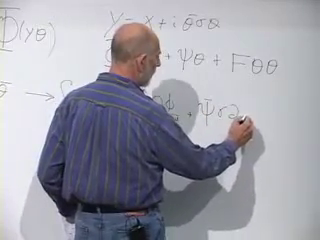
\includegraphics[width=0.76\textwidth]{lecture_09_figure_02.png}
\lectureframe{00:27:36.000}
\caption{手徵座標與分量展開；圖中標示了純量、費米子及輔助場項。}
\end{figure}

\section{\texorpdfstring{\(d^2\theta\)}{d2-theta}積分選出什麼}

相互作用與質量來自全純函數\(W(\Phi)\)，也就是超勢：
\begin{equation}
S_W
=
\int d^4x
\left[
\int d^2\theta\,W(\Phi)
+\mathrm{h.c.}
\right].
\label{eq:l9-superpotential-action}
\end{equation}
手徵表示式不獨立依賴\(\bar\theta\)，因此對全部四個反對易座標積分會得到零。\(d^2\theta\)積分則會選出其中的\(\theta^2\)分量。

先以一般函數之前的簡單例子說明組合方式，令\(W(\Phi)=\Phi^n\)。在
\begin{equation}
(\phi+\sqrt2\,\theta\psi+\theta^2F)^n,
\end{equation}
中，恰好得到兩個\(\theta\)的方式有兩種：可以選取一個\(F\theta^2\)，也可以選取兩個費米子因子。

\begin{classroomqa}
\audiencequestion{有多少項包含一個選定的\(F\theta^2\)，其餘因子則全是純量：是\(n-1\)個還是\(n\)個？\lecturetimestamp{00:31:33}}
\lecturerresponse{共有\(n\)項。\(n\)個因子中的任一個都可以提供\(F\theta^2\)，其餘\(n-1\)個因子則提供\(\phi\)。這些項的貢獻為\(nF\phi^{n-1}\)。}
\end{classroomqa}

\begin{classroomqa}
\audiencequestion{有多少種方式可由兩個因子提供兩個費米子？\lecturetimestamp{00:32:26}}
\lecturerresponse{共有\(\binom n2=n(n-1)/2\)種不計順序的選法。格拉斯曼縮併會決定相應的\(\psi\psi\)項。}
\end{classroomqa}

因此，按照講義中省略係數的記號，
\begin{equation}
\int d^2\theta\,\Phi^n+\mathrm{h.c.}
\;\leadsto\;
nF\phi^{n-1}
-\frac{n(n-1)}{2}\phi^{n-2}\psi\psi
+\mathrm{h.c.}
\label{eq:l9-power-extraction}
\end{equation}
此處的負號遵循標準的歸一化展開與格拉斯曼慣例；若採用不同慣例，表面上的符號可能有所不同。

\begin{classroomqa}
\audiencequestion{不含任何\(\theta\)的項\(\phi^n\)怎麼處理？\lecturetimestamp{00:33:10}}
\lecturerresponse{它確實出現在乘積中，但會被\(d^2\theta\)積分捨去。箭頭表示積分會選出\(\theta^2\)的係數；它不表示兩個完整表示式相等。}
\end{classroomqa}

\begin{figure}[H]
\centering
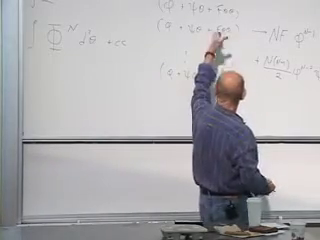
\includegraphics[width=0.82\textwidth]{lecture_09_figure_03.png}
\lectureframe{00:33:38.000}
\caption{重複的超場因子，以及表示取出它們的雙\(\theta\)分量、而非表示兩者相等的箭頭。}
\end{figure}

將帶有任意係數的各次冪加總後，組合因子便轉化為導數：
\begin{equation}
\int d^2\theta\,W(\Phi)+\mathrm{h.c.}
\;\leadsto\;
F W'(\phi)
-\frac12 W''(\phi)\psi\psi
+\mathrm{h.c.}
\label{eq:l9-W-components}
\end{equation}

\begin{classroomqa}
\audiencequestion{為什麼費米子項含有\(\phi^{n-2}\)，而不是\(\phi^{n-1}\)？\lecturetimestamp{00:36:32}}
\lecturerresponse{兩個因子已經提供費米子，剩下\(n-2\)個純量因子。因此係數是二階導數\(W''(\phi)\)的一半。}
\end{classroomqa}

費米子項相當重要：\(W''\)為常數時，它給出質量；\(W''\)依賴\(\phi\)時，它給出湯川相互作用。不過在分析真空時，輔助場項\(FW'\)提供了直接的資訊。

\section{消去輔助場}

整理出含有\(F\)的各項：
\begin{equation}
\mathcal L_F
=
F^\ast F
+F W'(\phi)
+F^\ast \overline{W'(\phi)}.
\label{eq:l9-LF}
\end{equation}
由於沒有\(\partial_\mu F\)項，完整的歐拉--拉格朗日方程
\begin{equation}
\partial_\mu
\frac{\partial\mathcal L}{\partial(\partial_\mu F)}
-
\frac{\partial\mathcal L}{\partial F}
=0
\end{equation}
會立即化為代數方程。將\(F\)與\(F^\ast\)視為獨立變數，可得
\begin{align}
\frac{\partial\mathcal L_F}{\partial F}
&=F^\ast+W'(\phi)=0,
&
\frac{\partial\mathcal L_F}{\partial F^\ast}
&=F+\overline{W'(\phi)}=0,
\label{eq:l9-F-eom}
\end{align}
因此
\begin{equation}
F^\ast=-W'(\phi),
\qquad
F=-\overline{W'(\phi)}.
\label{eq:l9-F-solution}
\end{equation}

\begin{figure}[H]
\centering
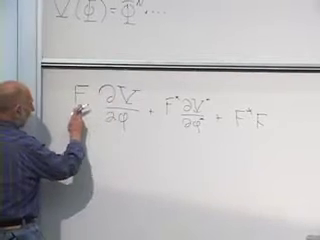
\includegraphics[width=0.82\textwidth]{lecture_09_figure_04.png}
\lectureframe{00:39:40.000}
\caption{板書遮擋移除後，完整的輔助場表示式及其代數運動方程一覽無遺。}
\end{figure}

\begin{classroomqa}
\audiencequestion{該導數應該對\(\phi\)取，而不是對黑板上寫的共軛場取嗎？\lecturetimestamp{00:41:21}}
\lecturerresponse{是的。修正後，式~\eqref{eq:l9-F-eom}中的共軛對便完整了：\(F^\ast=-W'(\phi)\)與\(F=-\overline{W'(\phi)}\)。}
\end{classroomqa}

代入式~\eqref{eq:l9-LF}可得
\begin{equation}
\mathcal L_F\big|_{\mathrm{on\ shell}}
=-|W'(\phi)|^2.
\end{equation}
由於純量拉格朗日量的形式是動能減去勢能，普通的純量勢為
\begin{equation}
\boxed{V(\phi,\phi^\ast)=|W'(\phi)|^2\ge0.}
\label{eq:l9-F-potential}
\end{equation}
這個\(V\)不是超勢。我們以\(W\)表示超空間中的全純函數，以\(V\)表示普通勢能。

\subsection{兩個直接例子}

採用標準的精確歸一化，
\begin{equation}
\begin{gathered}
W(\Phi)=\frac12m\Phi^2,\\
W'(\phi)=m\phi,
\qquad V=|m|^2|\phi|^2.
\end{gathered}
\label{eq:l9-quadratic-W}
\end{equation}
同一項也給出費米子質量
\(-\tfrac12m\psi\psi+\mathrm{h.c.}\)，因此超對稱破缺之前，純量與費米子的質量相同。

若取
\begin{equation}
W(\Phi)=\frac{g}{3}\Phi^3,
\end{equation}
則可得
\begin{equation}
\begin{gathered}
W'(\phi)=g\phi^2,
\qquad V=|g|^2|\phi|^4,\\
\mathcal L_{\mathrm{Yukawa}}
=-g\phi\psi\psi+\mathrm{h.c.}
\end{gathered}
\label{eq:l9-cubic-W}
\end{equation}
四純量頂點描述兩個純量的散射，而湯川項則是與之相應的超對稱項。

\section{兩種真空}

真空是\(V\)取極小值時的常數場構型；此時導數項為零。由於式~\eqref{eq:l9-F-potential}非負，可能的情況有兩種。

\subsection{零能量極小值}

若存在某個\(\phi_0\)滿足
\begin{equation}
W'(\phi_0)=0,
\end{equation}
則
\begin{equation}
V(\phi_0)=0,
\qquad
\langle F\rangle=0.
\label{eq:l9-unbroken-F}
\end{equation}
此真空具有超對稱性。這類似磁化強度為零的情況：沒有輔助場分量選定超空間方向。

\subsection{能量抬升的極小值}

若方程
\begin{equation}
W'(\phi)=0
\label{eq:l9-F-flatness}
\end{equation}
在極小值處沒有共同解，則
\begin{equation}
V_{\min}>0,
\qquad
\langle F\rangle\neq0,
\label{eq:l9-broken-F}
\end{equation}
超對稱便自發破缺。作用量仍具有超對稱性，但其最低能量態沒有。

\begin{figure}[H]
\centering
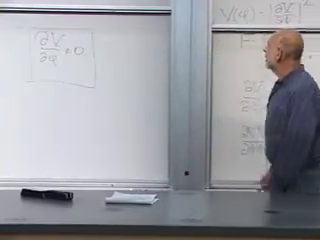
\includegraphics[width=0.88\textwidth]{lecture_09_figure_05.png}
\lectureframe{00:52:09.960}
\caption{板書同時列出正定的勢、\(F\)方程與真空條件，並呈現對稱的方程如何導出不具對稱性的解。}
\end{figure}

透過費米子變換，可以精確表述序參量的意義：
\begin{equation}
\delta\psi_\alpha
=
i\sqrt2
(\sigma^\mu\bar\epsilon)_\alpha\partial_\mu\phi
+\sqrt2\,\epsilon_\alpha F.
\label{eq:l9-fermion-transformation}
\end{equation}
對均勻真空而言，導數項為零。若\(\langle F\rangle\neq0\)，超對稱變換就會使費米子產生非零的常數位移，因此真空不可能保持不變。\editorialnote{方程~\eqref{eq:l9-fermion-transformation}是標準的分量形式，明確呈現講課中所說的超場分量會彼此變換。}

同樣的結論也可由超代數導出。在靜止系中，
\begin{equation}
\{Q_\alpha,Q_{\dot\alpha}^\dagger\}
=2\sigma^0_{\alpha\dot\alpha}H.
\end{equation}
取真空期望值後，真空能量可表示為超荷作用於真空所得各態的範數平方總和：
\begin{equation}
E_0\ge0,
\qquad
E_0=0
\ \Longleftrightarrow\
Q_\alpha|0\rangle
=Q_{\dot\alpha}^\dagger|0\rangle=0.
\label{eq:l9-algebra-vacuum-energy}
\end{equation}
因此，在剛性超對稱理論中，真空能為正與超對稱自發破缺是同一件事的兩面。

\begin{center}
\begin{tikzpicture}[x=1.2cm,y=1.0cm,>=Latex]
  \draw[->] (-3,0) -- (-0.2,0) node[right] {\(\phi\)};
  \draw[->] (-2.8,-0.15) -- (-2.8,2.1) node[above] {\(V\)};
  \draw[thick,teal!75!black,domain=-2.5:-0.5,samples=60]
    plot (\x,{0.65*(\x+1.5)^2});
  \fill (-1.5,0) circle (2pt);
  \node[below] at (-1.5,0) {\(F=0\)};
  \draw[->] (0.4,0) -- (3.2,0) node[right] {\(\phi\)};
  \draw[->] (0.6,-0.15) -- (0.6,2.1) node[above] {\(V\)};
  \draw[thick,orange!85!black,domain=0.9:2.9,samples=60]
    plot (\x,{0.55*(\x-1.9)^2+0.65});
  \fill (1.9,0.65) circle (2pt);
  \draw[dashed] (0.6,0.65) -- (1.9,0.65);
  \node[below] at (1.9,0.65) {\(F\neq0\)};
\end{tikzpicture}
\end{center}

\editorialnote{一個最簡單的例子是\(W=f\Phi\)；其中\(W'=f\)永不為零，而且\(V=|f|^2\)。這個單場例子具有平坦的純量方向；若要實現穩定的\(F\)項破缺，通常需要多個手徵場，例如 O'Raifeartaigh 型隱藏部門。}

\section{超對稱破缺會產生什麼}

\subsection{質量分裂}

鐵磁體的類比在此再次回到譜上。弱內部磁場會使原子能階分裂，卻不會改變原子的本質。同樣地，弱耦合傳遞的超對稱破缺序參量，會使原本同屬一個超多重態的玻色子與費米子質量分裂。

\begin{classroomqa}
\audiencequestion{超對稱會使哪些粒子彼此轉換，因此真空破缺超對稱時，這些粒子會失去質量簡併？\lecturetimestamp{00:51:40}}
\lecturerresponse{玻色子與費米子。當狀態不再遵循聯繫兩者的變換時，它們的質量便不必相等。}
\end{classroomqa}

單靠\(\langle F\rangle\)並不會造成質量分裂；還需要能將破缺效應傳遞至可見場的耦合。若這些耦合很弱，可見粒子仍能清楚辨認，質量分裂也遠小於大統一或普朗克尺度。若耦合很強，情況就像原子受到巨大磁場扭曲，變成細長而難以辨認的物體。

\subsection{戈德斯通費米子}

對於一般的破缺生成元，\(J|0\rangle\)會產生玻色型戈德斯通態。超荷是費米型的，會將玻色態轉變為費米態。由於真空被視為玻色態，破缺的超荷會產生一個費米型零能態：
\begin{equation}
Q_\alpha|0\rangle
\sim
|\widetilde G_\alpha,\mathbf k=0\rangle.
\label{eq:l9-goldstino}
\end{equation}
其傳播態是無質量外爾費米子，也就是戈德斯通費米子，或稱戈德斯通微子。

\begin{classroomqa}
\audiencequestion{若超對稱變換不使真空保持不變，會產生什麼新態？\lecturetimestamp{00:53:24}}
\lecturerresponse{無質量費米子。一般戈德斯通定理的模式依然成立，但費米型生成元會將玻色型真空轉變為戈德斯通費米子。}
\end{classroomqa}

因此，剛性超對稱自發破缺必然有兩種表徵：
\begin{equation}
\boxed{
V_{\min}>0
\qquad\text{and}\qquad
\text{a massless goldstino}.
}
\label{eq:l9-rigid-breaking-signatures}
\end{equation}

\section{隱藏部門}

將原子與鐵磁體視為兩個部門，是很有用的看法。鐵磁體形成序參量，原子感受到的則是從鐵磁體傳遞而來的場。耦合很弱時，操控原子幾乎不會激發磁振子，也很難直接探測磁性介質。因此鐵磁體是隱藏的，但可從微小的譜線分裂推知它的存在。

超對稱模型建構也採用相同的說法。隱藏部門中的額外場會形成非零的\(F\)項或\(D\)項期望值。稱為媒介機制的相互作用會將破缺效應傳至可見部門，並為超伴粒子產生軟質量。效應傳遞微弱，可以解釋為何可見理論在遠高於低能尺度的基本尺度上仍近似具有超對稱性，但低能下的玻色子--費米子質量並不完全簡併。

這種架構並非自動成立；它需要額外場、穩定的破缺真空，以及可受控的媒介機制。因此講課將現實中的超對稱破缺描述為複雜且多少有些牽強，而非最小模型必然導出的單一結果。

\section{引力會改變這兩種表徵}

\subsection{真空能成為引力源}

沒有引力時，將所有能量加上一個常數，不會改變非引力實驗的結果。有引力時，真空能量密度會以宇宙學常數的形式進入愛因斯坦方程。正的\(V_{\min}\)會驅動加速膨脹。若其尺度與超伴粒子質量所需的粒子物理尺度相當，所產生的曲率便會遠遠大於觀測值。

\begin{classroomqa}
\audiencequestion{納入引力後，正的非零真空能會對宇宙造成什麼影響？\lecturetimestamp{01:00:40}}
\lecturerresponse{它會像宇宙學常數一樣，驅動加速膨脹。若真空能處於一般粒子物理尺度，其效應就會大得令人無法接受。}
\end{classroomqa}

局域超對稱，也就是超引力，會改變正定平方和的公式。為便於掌握，標準的\(N=1\) \(F\)項勢能為
\begin{equation}
\begin{aligned}
V_F={}&e^{K/M_P^2}
\left(
K^{i\bar j}D_iW\,D_{\bar j}\overline W
-\frac{3|W|^2}{M_P^2}
\right),\\
D_iW={}&\partial_iW+\frac{\partial_iK}{M_P^2}W.
\end{aligned}
\label{eq:l9-sugra-potential}
\end{equation}
由於存在負項，原則上可以部分抵銷超對稱破缺所產生的正能量。剩餘部分可能形成很小的宇宙學常數。

\editorialnote{講課刻意只給出示意性的修正，並明確對普朗克質量的放置方式提出疑問。方程~\eqref{eq:l9-sugra-potential}列出具有 Kähler 勢\(K\)的手徵多重態所適用的標準公式；規範\(D\)項還會帶來額外的非負貢獻。這個公式並未解釋觀測到的極小值；這仍是宇宙學常數問題。}

\subsection{超希格斯機制}

第二個引力效應可從極化態的計數來理解。一個自旋為\(j\)的有質量粒子，在靜止系中有\(2j+1\)個自旋態。

\begin{classroomqa}
\audiencequestion{有質量且自旋為\(j\)的粒子有多少個自旋態？\lecturetimestamp{01:05:16}}
\lecturerresponse{\(2j+1\) 個。特別是，有質量的自旋 1 粒子有三個態；而無質量規範玻色子只有螺旋度 \(+1\) 和 \(-1\)。}
\end{classroomqa}

這是運動學上的差別。有質量粒子可以經由洛侖茲變換到達靜止系，再以不同方向運動，同時保持自旋取向，因此所有自旋投影都必須存在。無質量粒子無法被超越，也無法帶到靜止。因此它只能具有兩種極端螺旋度。

對電弱規範場而言，
\begin{equation}
\underbrace{(+1,-1)}_{\text{massless vector}}
+
\underbrace{(0)}_{\text{Goldstone}}
\longrightarrow
\underbrace{(+1,0,-1)}_{\text{massive vector}}.
\label{eq:l9-higgs-count}
\end{equation}

\begin{classroomqa}
\audiencequestion{有質量\(W\)或\(Z\)的縱向極化從何而來？\lecturetimestamp{01:08:50}}
\lecturerresponse{來自戈德斯通玻色子。它被規範場吸收，補足有質量自旋 1 表示所需的三個態。}
\end{classroomqa}

引力具有無質量自旋 2 的引力子。它的超對稱夥伴是無質量、自旋為\(\tfrac32\)的引力微子。

\begin{classroomqa}
\audiencequestion{引力子的自旋是多少？它的超對稱夥伴自旋又是多少？\lecturetimestamp{01:10:24}}
\lecturerresponse{引力子的自旋為\(2\)；費米子夥伴的自旋相差二分之一，為\(3/2\)。}
\end{classroomqa}

無質量引力微子的螺旋度為\(\pm\tfrac32\)；有質量引力微子還必須具有\(\pm\tfrac12\)。戈德斯通微子恰好提供這些缺少的態：
\begin{equation}
\begin{gathered}
\underbrace{\left(+\frac32,-\frac32\right)}_{\text{massless gravitino}}
\oplus
\underbrace{\left(+\frac12,-\frac12\right)}_{\text{goldstino}}\\
\Downarrow\\
\underbrace{\left(+\frac32,+\frac12,-\frac12,-\frac32\right)}_{\text{massive gravitino}}.
\end{gathered}
\label{eq:l9-super-higgs}
\end{equation}
這就是超希格斯機制。超對稱一旦成為局域對稱，戈德斯通微子便會被吸收，不再以獨立的無質量粒子出現。由此形成的引力微子透過引力作用，因此很難產生。

\section{轉換主題：為什麼選擇\texorpdfstring{\(SU(5)\)}{SU(5)}？}

接下來從超對稱形式體系轉向大統一。標準模型的規範群為
\begin{equation}
G_{\mathrm{SM}}
=SU(3)_c\times SU(2)_L\times U(1)_Y.
\label{eq:l9-sm-group}
\end{equation}
其三個因子分別描述色、弱同位旋與弱超荷。大統一要探討的是：這個乘積群是否是一個更大單群的剩餘子群，使表面上各自分離的粒子多重態與規範作用力都成為同一結構的一部分。此處要討論的最小候選群是\(SU(5)\)。

\subsection{群元素與生成元}

對於\(U\in SU(N)\)，
\begin{equation}
U^\dagger U=\mathbf1,
\qquad
\det U=1.
\label{eq:l9-SUN-def}
\end{equation}
第一個條件表示么正性；第二個條件則定義了「特殊」群。將無窮小群元素寫成
\begin{equation}
U=\mathbf1+i\epsilon G+\mathcal O(\epsilon^2).
\label{eq:l9-infinitesimal-U}
\end{equation}
么正性要求
\begin{equation}
G^\dagger=G,
\end{equation}
而
\begin{equation}
\det e^{i\epsilon G}
=e^{i\epsilon\operatorname{tr}G}=1
\end{equation}
則要求
\begin{equation}
\operatorname{tr}G=0.
\end{equation}
因此，生成元是無跡的厄米矩陣。

一個\(N\times N\)厄米矩陣含有\(N^2\)個實參數：\(N\)個實對角元，以及\(N(N-1)/2\)個複數非對角元。無跡條件會去掉一個參數。因此
\begin{equation}
\dim SU(N)=N^2-1,
\qquad
\dim SU(5)=24.
\label{eq:l9-SU5-dimension}
\end{equation}
作為比較，\(SU(2)\)有三個泡利生成元，\(SU(3)\)則有八個色生成元。

\section{\texorpdfstring{\(SU(5)\)}{SU(5)}中的標準模型基本組件}

將五維空間分成弱同位旋的二維區塊與色的三維區塊：
\begin{equation}
\mathbf5=\mathbf2\oplus\mathbf3.
\end{equation}
嵌入的生成元形式如下：
\begin{align}
T^a_L
&=
\begin{pmatrix}
\tfrac12\tau^a&0\\
0&0_{3\times3}
\end{pmatrix},
&& a=1,2,3,
\label{eq:l9-SU2-block}\\
T^A_c
&=
\begin{pmatrix}
0_{2\times2}&0\\
0&\tfrac12\lambda^A
\end{pmatrix},
&& A=1,\ldots,8.
\label{eq:l9-SU3-block}
\end{align}
泡利矩陣\(\tau^a\)生成弱\(SU(2)\)；蓋爾曼矩陣\(\lambda^A\)生成色\(SU(3)\)。由於兩個區塊互不重疊，這兩個子群彼此對易。

另一個對角生成元在每個區塊內都正比於單位矩陣，因此與兩者皆對易。在基本表示中，一種方便的雙倍超荷慣例為
\begin{equation}
T_Y^{(\mathbf5)}=
\operatorname{diag}
\left(
1,1,-\frac23,-\frac23,-\frac23
\right).
\label{eq:l9-hypercharge-generator}
\end{equation}
其跡為零：
\begin{equation}
1+1-3\left(\frac23\right)=0.
\end{equation}
共軛物質表示的本徵值符號相反：
\begin{equation}
Y_{\overline{\mathbf5}}
=
\operatorname{diag}
\left(
-1,-1,\frac23,\frac23,\frac23
\right),
\label{eq:l9-fivebar-hypercharge}
\end{equation}
這些數值就是講義中物質欄所列的值。整體符號與歸一化皆屬慣例；此處採用標準模型慣例
\begin{equation}
Q=T_3+\frac{Y}{2}.
\label{eq:l9-charge}
\end{equation}
方程~\eqref{eq:l9-SU2-block}--\eqref{eq:l9-hypercharge-generator}展示了
\begin{equation}
SU(3)_c\times SU(2)_L\times U(1)_Y
\subset SU(5).
\end{equation}

三個弱作用生成元、八個色生成元和一個超荷生成元，合計為\(12\)個，佔\(24\)個\(SU(5)\)生成元中的一半。\editorialnote{其餘十二個生成元位於非對角的\(2\times3\)區塊和\(3\times2\)區塊。它們所對應的規範玻色子會在夸克型分量與輕子型分量之間進行轉換；這正是後續將探討的重子數與輕子數改變相互作用的結構性起源。}

\begin{classroomqa}
\audiencequestion{哪些規範粒子對應於熟悉的子群生成元？\lecturetimestamp{01:31:05}}
\lecturerresponse{八個\(SU(3)\)生成元對應八個膠子。三個\(SU(2)\)生成元對應弱規範場；經過電弱混合後，這些場成為\(W^\pm\)，以及\(Z\)－光子系統中的一部分；\(U(1)\)場則提供另一個中性組合。}
\end{classroomqa}

\section{以左手場描述一代粒子}

聚焦於第一代；{\proseunicodefont μ}子／粲夸克／奇夸克代，以及{\proseunicodefont τ}子／頂夸克／底夸克代，也都遵循相同模式。最簡潔的計數方式，是將每個獨立的維爾場都視為左手場。右手粒子則以其左手電荷共軛場表示：
\begin{equation}
Q_L=(u_L,d_L),\quad
L_L=(\nu_{eL},e_L),\quad
u^c_L,\quad d^c_L,\quad e^c_L.
\end{equation}
它們的重數如下：
\begin{equation}
\underbrace{6}_{Q_L}
+
\underbrace{2}_{L_L}
+
\underbrace{3}_{u^c_L}
+
\underbrace{3}_{d^c_L}
+
\underbrace{1}_{e^c_L}
=15.
\label{eq:l9-fifteen-fields}
\end{equation}

\editorialnote{最小標準模型不包含獨立的右手中微子維爾場，因此場的數目為\(15\)。僅憑這項計數，不能據此斷言中微子是馬約拉納粒子。加入一個單態場\(\nu^c_L\)後，場的數目便成為\(16\)，並自然引向\(SO(10)\)，這已超出目前\(SU(5)\)構造的範圍。}

五維多重態必須將無色的弱二重態分量置於前兩個位置，並將有色的弱單態分量置於後三個位置。

\begin{classroomqa}
\audiencequestion{所提出的欄向量包含六個場，而不是五個嗎？\lecturetimestamp{01:36:14}}
\lecturerresponse{不是。第一輪寫下的上夸克已被刪去。這個欄向量包含中微子、電子，以及反下夸克的三種顏色態，總共五個分量。}
\end{classroomqa}

因此得到
\begin{equation}
\overline{\mathbf5}
=
\begin{pmatrix}
\nu_{eL}\\
e_L\\
d^c_{rL}\\
d^c_{gL}\\
d^c_{bL}
\end{pmatrix}.
\label{eq:l9-fivebar}
\end{equation}
\editorialnote{講義起初只稱它為五維多重態。依照標準的全左手\(SU(5)\)記號，其色與超荷指派顯示它屬於共軛表示\(\overline{\mathbf5}\)。}
前兩個分量在\(SU(2)_L\)變換下會改變，但不帶色荷。後三個分量在色變換下屬於反三重態，但都是弱單態。

\begin{classroomqa}
\audiencequestion{當所有場都寫成左手場時，哪些夸克帶有色荷，卻不帶弱\(SU(2)_L\)量子數？\lecturetimestamp{01:40:13}}
\lecturerresponse{右手夸克的電荷共軛場。對這個五分量多重態而言，依電荷判定，符合條件的是三個反下夸克場\(d^c_{r,g,b}\)。}
\end{classroomqa}

式~\eqref{eq:l9-fivebar}中的電荷總和為零：
\begin{equation}
0-1+\frac13+\frac13+\frac13=0.
\label{eq:l9-fivebar-charge-sum}
\end{equation}
這是必要的，因為電荷算符是\(SU(5)\)生成元的無跡組合。

\begin{classroomqa}
\audiencequestion{為什麼三個色分量是反下夸克，而不是反上夸克？\lecturetimestamp{01:43:38}}
\lecturerresponse{中微子和電子的總電荷為\(-1\)。三種顏色的反下夸克總電荷為\(+1\)，使總和為零。若換成三個反上夸克場，總電荷就會不對。}
\end{classroomqa}

剩下的十個左手場為
\begin{equation}
Q_L\;(6)
\oplus
u^c_L\;(3)
\oplus
e^c_L\;(1),
\end{equation}
它們恰好組成反對稱二階表示
\begin{equation}
\mathbf{10}\cong\wedge^2\mathbf5,
\qquad
\dim\wedge^2\mathbf5=\binom52=10.
\label{eq:l9-ten-preview}
\end{equation}
如何明確地將這些場配置於表示中，是下一講的任務。每一代標準模型粒子都符合這項數目上的吻合：
\begin{equation}
\overline{\mathbf5}\oplus\mathbf{10}
\end{equation}
這是\(SU(5)\)構想並非任意重新標記的第一個顯著證據。

\begin{classroomqa}
\audiencequestion{如果五重態和十重態是不同的表示，是否代表其中的粒子不能互相作用？\lecturetimestamp{01:46:14}}
\lecturerresponse{不會。群變換在各自的不可約表示內作用，因此不會直接將五重態中的成員變換成十重態中的成員。不過，這兩組場仍可透過發射與吸收共同的規範玻色子而互相作用，希格斯耦合也能連結它們。}
\end{classroomqa}

\section{回顧與展望}

本講追蹤了一個橫跨迥異尺度的相同模式。旋轉不變性使原子能階簡併；磁場背景則使能階分裂。鐵磁體會產生這樣的背景，同時使底層定律維持對稱；無能隙磁振子的存在，則顯示不對稱性出現在真空中。在手徵超對稱理論裡，輔助場的期望值扮演序參量的角色：
\begin{equation}
\begin{aligned}
\langle F\rangle=0
&\quad\Longleftrightarrow\quad
\text{unbroken supersymmetry},\\
\langle F\rangle\neq0
&\quad\Longrightarrow\quad
\text{spontaneous breaking}.
\end{aligned}
\end{equation}
在剛性超對稱下，對稱性破缺的真空具有正能量，會使超多重態分裂，並產生戈德斯通費米子。弱作用媒介機制促使人們引入隱藏部門；引力則使真空能成為宇宙學問題，並將戈德斯通費米子吸收進有質量的引力微子。

結尾的\(SU(5)\)構造開啟了一個新問題，並未將它解決。無跡厄米\(5\times5\)生成元包含標準模型的各個區塊，而前五個物質場恰好可嵌入為
\((\nu_e,e^-,d^c_r,d^c_g,d^c_b)\)。其餘十個場則位於反對稱表示中，尚待安排。這項尚未完成的嵌入，正是大統一理論真正開始之處。

\chapter{\texorpdfstring{\(SU(5)\)}{SU(5)} 多重態、輕子夸克規範玻色子與質子衰變}

\lectureoverview{標準模型群嵌入 \(SU(5)\) 後，大統一便有了具體形式。為了理解這項陳述的意義，我們先建立所需的表示論基礎：定義表示 \(N\)、其共軛表示 \(\overline N\)、張量積、對稱與反對稱張量，以及伴隨表示。標準模型的一個世代，竟可整合為相當精簡的組合 \(\overline{\mathbf 5}\oplus\mathbf{10}\)。使這種安排如此優美的同一對稱性，也要求存在能使夸克與輕子互相轉換的帶色規範玻色子。這些玻色子的交換使質子衰變成為可能，因而將統一能標推向 \(10^{15}\)--\(10^{16}\,\mathrm{GeV}\)。規範耦合的跑動也指向相近的能標；最後還會談到超對稱，因為納入超對稱後，三種耦合的數值交會會明顯更精確。}

\section{為什麼要從群表示談起？}

大統一理論有許多種提案。我們不逐一綜述，而是拆解其中一個例子，探討三個問題：它為何可行、它要求哪些新粒子，以及實驗在哪些方面對它構成威脅。這個群是 \(SU(5)\)，其關鍵結構特徵是以下嵌入關係
\begin{equation}
SU(3)_c\times SU(2)_L\times U(1)_Y
\subset SU(5).
\label{eq:l10-sm-embedding}
\end{equation}
其中 \(SU(3)_c\) 作用於色，\(SU(2)_L\) 作用於弱同位旋，而 \(U(1)_Y\) 作用於超荷。

超對稱並非這套建構的前提。超對稱與大統一在邏輯上互不蘊含。本講中兩者的關聯在於數值：把超伴子譜納入重整化群計算後，三種規範耦合會更精確地趨近同一個值。

受對稱性作用而彼此互相轉換的粒子，構成該對稱群的一個表示。因此，要分類統一理論中的粒子多重態，得先了解一些表示論。

\subsection{\texorpdfstring{\(SU(2)\)}{SU(2)} 的熟悉例子}

與普通角動量相關的 \(SU(2)\)，和三維空間的旋轉密切相關。更精確地說，\(SU(2)\) 是 \(SO(3)\) 的雙重覆蓋。其不可約表示以
\begin{equation}
j=0,\frac12,1,\frac32,\ldots,
\qquad
\dim(j)=2j+1.
\label{eq:l10-su2-spins}
\end{equation}
為標記。因此，標量是單態，自旋為 \(\tfrac12\) 的粒子是雙重態，自旋為一的粒子是三重態。弱群 \(SU(2)_L\) 是另一種物理對稱性，雖然兩者的抽象群論相同。

\section{定義表示及其共軛表示}

對於 \(SU(N)\)，定義表示的空間由複數 \(N\) 維列向量構成：
\begin{equation}
\psi=
\begin{pmatrix}
\psi_1\\
\psi_2\\
\vdots\\
\psi_N
\end{pmatrix},
\qquad
\psi'_i=U_i{}^j\psi_j,
\qquad
U\in SU(N).
\label{eq:l10-defining}
\end{equation}
它稱為定義表示，也簡稱為 \(\mathbf N\)。矩陣 \(U\) 的大小為 \(N\times N\)，其作用的向量空間維度則為 \(N\)。

複共軛會給出另一個 \(N\) 維表示：
\begin{equation}
\psi_i^*\longmapsto U_i{}^{j*}\psi_j^*,
\label{eq:l10-conjugate}
\end{equation}
此表示記為 \(\overline{\mathbf N}\)。當 \(N>2\) 時，定義表示與共軛表示並不等價。可以互換哪一個稱為粒子表示、哪一個稱為反粒子表示；但一旦選定約定，就必須始終一致。

\begin{classroomqa}
\audiencequestion{\(SU(N)\) 中的 \(N\)，會因 \(N\) 是偶數或奇數而異嗎？它指的是矩陣嗎？\lecturetimestamp{00:07:33}}
\lecturerresponse{這裡沒有偶--奇的限制。\(N\) 是定義矩陣的大小，也是定義表示的維度。\(\mathbf N\) 和 \(\overline{\mathbf N}\) 的維度都相同。}
\end{classroomqa}

反粒子的反粒子就是原來的粒子。因此，互換 \(\mathbf N\) 與 \(\overline{\mathbf N}\) 的名稱，只是改變約定，不會改變物理。

\section{張量積與不可約性}

假設一個物體有 \(N\) 種內部態，另一個物體也可獨立地處於相同數目的內部態。忽略位置、動量、自旋，以及除了 \(SU(N)\) 標記以外的所有量子數，這一對物體共有
\begin{equation}
N\times N=N^2
\label{eq:l10-product-count}
\end{equation}
種態。若第一個物體處於態 \(\psi_i\)，第二個處於態 \(\phi_j\)，兩者的乘積可寫成
\begin{equation}
\Psi_{ij}=\psi_i\phi_j,
\qquad
\Psi'_{ij}=U_i{}^kU_j{}^\ell\Psi_{k\ell}.
\label{eq:l10-tensor-transform}
\end{equation}
這就是張量積 \(\mathbf N\otimes\mathbf N\)。

\begin{classroomqa}
\audiencequestion{答案為 \(N^2\)，而不是 \(N^2-1\)，這是為什麼？允許兩個粒子具有相同的內部標記，會違反不相容原理嗎？\lecturetimestamp{00:10:22}}
\lecturerresponse{這裡的兩個位置可以區分：一個物體固定在一處，另一個固定在別處。泡利不相容原理約束的是包含位置在內的完整量子態，不會排除這些 \(N^2\) 種內部標記組合中的任何一種。數目 \(N^2-1\) 則會在稍後的另一種乘積中，因無跡條件而出現。}
\end{classroomqa}

\(N^2\) 維乘積表示通常是可約的。如果一個表示包含某個真子空間，且群的作用會將該子空間映回自身，這個表示便是可約的。可以將這些不變子空間分離出來，視為較小的表示；若不存在這種真子空間，該表示便是不可約的。

\subsection{對稱張量與反對稱張量}

每個二階張量都可唯一分解為
\begin{align}
\Psi_{ij}
&=\Psi^{(S)}_{ij}+\Psi^{(A)}_{ij},\\
\Psi^{(S)}_{ij}
&=\frac12(\Psi_{ij}+\Psi_{ji}),\\
\Psi^{(A)}_{ij}
&=\frac12(\Psi_{ij}-\Psi_{ji}).
\label{eq:l10-sym-anti}
\end{align}
這兩部分分別滿足
\begin{equation}
\Psi^{(S)}_{ij}=\Psi^{(S)}_{ji},
\qquad
\Psi^{(A)}_{ij}=-\Psi^{(A)}_{ji}.
\end{equation}
式~\eqref{eq:l10-tensor-transform}使兩種條件各自保持不變，因此群變換不會將對稱部分與反對稱部分互相混合。

\editorialnote{講義將一般情形的計數留作練習。對稱部分與反對稱部分的維度分別為 \(N(N+1)/2\) 和 \(N(N-1)/2\)，兩者相加為 \(N^2\)。}

\begin{figure}[htbp]
\centering
\includegraphics[width=0.78\textwidth]{lecture_10_figure_02.png}
\lectureframe{00:17:57.500}
\caption{兩個自旋為 \(\tfrac12\) 的態所構成的完整分解：三個對稱態與一個反對稱態。}
\label{fig:l10-spin-decomposition}
\end{figure}

對於 \(SU(2)\) 的定義二重態，
\begin{equation}
\mathbf2\otimes\mathbf2=\mathbf3_S\oplus\mathbf1_A.
\label{eq:l10-two-two}
\end{equation}
若以 \(u\) 和 \(d\) 表示兩個基底態，對稱三重態為
\begin{align}
\ket{1,1}&=\ket{uu},\\
\ket{1,0}&=\frac{1}{\sqrt2}\bigl(\ket{ud}+\ket{du}\bigr),\\
\ket{1,-1}&=\ket{dd},
\end{align}
反對稱單態則為
\begin{equation}
\ket{0,0}
=\frac{1}{\sqrt2}\bigl(\ket{ud}-\ket{du}\bigr).
\end{equation}
這就是熟悉的兩個自旋為 \(\tfrac12\) 的角動量相加：四個原始態重新組合成自旋一態與自旋零態。

\section{粒子與反粒子：伴隨表示}

現在將定義表示與其共軛表示相乘。此乘積仍有 \(N^2\) 個分量，但變換方式如同矩陣：
\begin{equation}
M_i{}^j\in\mathbf N\otimes\overline{\mathbf N},
\qquad
M\longmapsto U M U^\dagger.
\label{eq:l10-matrix-transform}
\end{equation}
這和 \(\mathbf N\otimes\mathbf N\) 不同；一個基本表示指標與一個反基本表示指標之間，沒有有意義的交換對稱性。自然的分解方式是
\begin{equation}
M
=
\frac{\operatorname{tr}M}{N}\,\mathbf1_N
+
\left(M-\frac{\operatorname{tr}M}{N}\,\mathbf1_N\right).
\label{eq:l10-trace-split}
\end{equation}
第一項是單態，無跡部分則是伴隨表示：
\begin{equation}
\mathbf N\otimes\overline{\mathbf N}
=\mathbf1\oplus\mathbf{Adj},
\qquad
\dim\mathbf{Adj}=N^2-1.
\label{eq:l10-adjoint}
\end{equation}

\begin{figure}[htbp]
\centering
\includegraphics[width=0.67\textwidth]{lecture_10_figure_04.png}
\lectureframe{00:23:47.500}
\caption{黑板上的結論：\(\mathbf N\otimes\overline{\mathbf N}\) 的無跡部分由 \(N^2-1\) 個分量構成伴隨表示。}
\label{fig:l10-adjoint}
\end{figure}

對於 \(SU(3)\)，這會得到熟悉的八重態：
\begin{equation}
\mathbf3\otimes\overline{\mathbf3}
=\mathbf8\oplus\mathbf1,
\end{equation}
八個膠子在伴隨表示下變換。對於 \(SU(2)\)，伴隨表示的維度為三，其變換方式如同自旋一態。

\section{標準模型的一個世代}

我們觀測到三個世代，但 \(SU(5)\) 對每個世代分別重複相同的建構，並未解釋為何有三個世代。因此，我們聚焦於第一代。

所有場都以左手 Weyl 場表示。右手費米子則以其左手電荷共軛場表示：
\begin{equation}
u^c_L,\qquad d^c_L,\qquad e^c_L.
\label{eq:l10-left-handed-bookkeeping}
\end{equation}
上標 \(c\) 表示電荷共軛。例如，\(d^c_L\) 是電荷為 \(+\tfrac13\) 的左手反下夸克場。

按照標準的 \(SU(5)\) 記號，十五個左手場中有五個組成
\begin{equation}
\overline{\mathbf5}
=
\begin{pmatrix}
\nu_{eL}\\
e_L\\
d^c_{rL}\\
d^c_{gL}\\
d^c_{bL}
\end{pmatrix}.
\label{eq:l10-fivebar}
\end{equation}
排列方式是先放入弱作用的二維區塊，再接著放入色作用的三維區塊。弱作用變換會混合前兩個分量，色變換則混合最後三個分量；非對角的 \(SU(5)\) 生成元會連結這兩個區塊。

\editorialnote{講義將式~\eqref{eq:l10-fivebar}中的欄向量稱為 \(\mathbf5\)，之後又將反對稱多重態稱為 \(\overline{\mathbf{10}}\)。這是將所有表示整體共軛的約定。我們採用現代標準約定 \(\overline{\mathbf5}\oplus\mathbf{10}\)；將每個表示取共軛，就能得到講義中的標記，而不改變物理內容。}

第一代的完整最小粒子清單為
\begin{equation}
\begin{gathered}
\underbrace{Q_L=(u_L,d_L)}_{6}
\oplus
\underbrace{L_L=(\nu_{eL},e_L)}_{2},\\
\underbrace{u^c_L}_{3}
\oplus
\underbrace{d^c_L}_{3}
\oplus
\underbrace{e^c_L}_{1},\\
6+2+3+3+1=15.
\end{gathered}
\label{eq:l10-fifteen}
\end{equation}
最小標準模型中沒有獨立的 \(\nu^c_L\)，因此無法產生可重整化的中微子質量。中微子振盪顯示這個最小模型並不完整：自然界中的中微子具有微小但非零的質量，因此需要擴充模型。

\begin{classroomqa}
\audiencequestion{費米子質量使左手態轉變為右手態時，也會使粒子變成反粒子嗎？\lecturetimestamp{00:34:00}}
\lecturerresponse{不會。電子質量項會連結左手電子與具有相同電荷的右手電子。在全左手記號中，後者以 \(e^c_L\) 表示，但四分量描述中的粒子仍然是電子。只有中性場才可能具有將粒子與反粒子視為同一者的 Majorana 質量。}
\end{classroomqa}

\section{五重態中可見的規範玻色子}

每個規範對稱性的生成元都對應一個規範場。在式~\eqref{eq:l10-fivebar}中，已可辨認出熟悉的轉換：
\begin{itemize}
\item 弱規範場作用於 \(\nu_{eL}\) 與 \(e_L\) 之間；
\item 膠子作用於 \(d^c_L\) 的三種顏色之間；
\item 中性生成元以對角方式作用；
\item 新的非對角生成元會將輕子分量轉變為帶色分量，或反向轉變。
\end{itemize}

可以將膠子想成攜帶夸克--反夸克的色量子數。講義使用常見的世界線助記法：沿著一條出射反夸克的世界線，從發射頂點往回追蹤，會看到它彷彿是正向運動的夸克。因此，發射出的場攜帶夸克--反夸克對的量子數。以表示論來說，這正是 \(\mathbf3\otimes\overline{\mathbf3}\) 的無跡部分。

對於 \(SU(5)\)，
\begin{equation}
\dim\mathbf{Adj}_{SU(5)}=5^2-1=24.
\end{equation}
這些規範場在標準模型子群下的分解為
\begin{equation}
\mathbf{24}
=
(\mathbf8,\mathbf1)_0
\oplus(\mathbf1,\mathbf3)_0
\oplus(\mathbf1,\mathbf1)_0
\oplus(\mathbf3,\mathbf2)_{-5/6}
\oplus(\overline{\mathbf3},\mathbf2)_{5/6},
\label{eq:l10-adjoint-sm}
\end{equation}
其中有序對表示 \(SU(3)_c\times SU(2)_L\)，下標表示超荷。

\editorialnote{式~\eqref{eq:l10-adjoint-sm}明確呈現講義所畫的區塊結構。前三項包含熟悉的色與電弱規範場；最後兩項包含十二個實自由度，慣稱為 \(X\) 與 \(Y\) 玻色子。}

\begin{figure}[htbp]
\centering
\begin{tikzpicture}[x=1.05cm,y=0.82cm]
  \draw[thick] (0,0) rectangle (5,5);
  \draw[thick] (2,0) -- (2,5);
  \draw[thick] (0,3) -- (5,3);
  \fill[blue!9] (0,3) rectangle (2,5);
  \fill[orange!10] (2,0) rectangle (5,3);
  \fill[teal!9] (2,3) rectangle (5,5);
  \fill[teal!9] (0,0) rectangle (2,3);
  \node[align=center] at (1,4) {weak and\\neutral fields};
  \node[align=center] at (3.5,1.5) {gluons and\\neutral field};
  \node[align=center] at (3.5,4) {\(X,Y\)};
  \node[align=center] at (1,1.5) {\(\overline X,\overline Y\)};
  \node[above] at (1,5) {\(2\)};
  \node[above] at (3.5,5) {\(3\)};
\end{tikzpicture}
\caption{\(SU(5)\)規範場的 \(2\oplus3\) 區塊結構。非對角區塊連結輕子與帶色場。}
\label{fig:l10-gauge-blocks}
\end{figure}

依據 \(Q=T_3+Y\)，式~\eqref{eq:l10-adjoint-sm}中的帶色弱二重態電荷為 \(-\tfrac13\) 和 \(-\tfrac43\)；其共軛態的電荷則為 \(+\tfrac13\) 和 \(+\tfrac43\)。講義將這些粒子稱為 \(X\) 和 \(Y\)，但明確表示不指定哪個名稱對應哪個電荷。物理上不變的是轉換過程與電荷。

\begin{classroomqa}
\audiencequestion{每種新的 \(X\) 或 \(Y\) 規範玻色子都有三種嗎？\lecturetimestamp{00:41:28}}
\lecturerresponse{是的。轉換會連結帶色夸克與無色輕子，因此交換的玻色子必須攜帶兩者之間缺少的色荷。\(X/Y\) 場形成色三重態，能發射或吸收膠子。}
\end{classroomqa}

帶色粒子不會以孤立的漸近態被觀測到。和夸克一樣，新的規範玻色子必須衰變或經歷強子化，形成色中性的組合。

\section{為什麼多重態中包含反下夸克}

\(SU(N)\)的生成元是無跡厄米矩陣。要看出這與「特殊」一詞的關聯，可將無窮小群元素寫為
\begin{equation}
U(\epsilon)=e^{i\epsilon T}.
\end{equation}
么正性給出 \(T^\dagger=T\)，而
\begin{equation}
1=\det U=e^{i\epsilon\operatorname{tr}T}
\end{equation}
對任意的 \(\epsilon\)，則可得
\begin{equation}
\operatorname{tr}T=0.
\label{eq:l10-traceless-generator}
\end{equation}

電荷是生成元的線性組合。在式~\eqref{eq:l10-fivebar}所示的物質欄向量上，它作用為
\begin{equation}
Q_{\overline5}
=
\operatorname{diag}
\left(0,-1,\frac13,\frac13,\frac13\right),
\qquad
\operatorname{tr}Q_{\overline5}=0.
\label{eq:l10-charge-fivebar}
\end{equation}
因此
\begin{equation}
0-1+3\left(\frac13\right)=0.
\end{equation}
若將反下夸克場換成下夸克場，則會得到
\begin{equation}
0-1+3\left(-\frac13\right)=-2,
\end{equation}
這不可能是 \(SU(5)\) 生成元的跡。因此，看似奇怪的反下夸克配置是群結構所強制的。

\section{其餘十個費米子}

另外十個場來自一個二階反對稱張量。在標準約定下，它是下式的反對稱部分：
\begin{equation}
\mathbf5\otimes\mathbf5
=\mathbf{15}_S\oplus\mathbf{10}_A.
\label{eq:l10-five-five}
\end{equation}
講義先暫時寫出共軛量子數
\begin{equation}
\chi=
\begin{pmatrix}
\nu^c\\
e^c\\
d_r\\
d_g\\
d_b
\end{pmatrix}.
\label{eq:l10-aux-five}
\end{equation}
再據此建構這個張量。這只是進行表示張量積時計算用的記帳方式，並非宣稱存在另一個由複合粒子構成的實體五重態。

令
\begin{equation}
\Psi^{ij}=-\Psi^{ji},
\qquad
i,j=1,\ldots,5.
\label{eq:l10-antisym-ten}
\end{equation}
所有對角元素皆為零，下三角部分則由上三角部分決定。因此
\begin{equation}
\dim\mathbf{10}
=\binom52
=\frac{5\cdot4}{2}
=10.
\label{eq:l10-ten-count}
\end{equation}

矩陣中每個分量的電荷，是式~\eqref{eq:l10-aux-five}中對應的列電荷與行電荷之和。由此可直接得到弱--弱位置上的 \(e^c\)、弱--色區塊中的下夸克和上夸克，以及色--色區塊中的反上夸克場。

\begin{classroomqa}
\audiencequestion{正電子和下夸克的標記組合後，所得分量應該是 \(X\) 玻色子嗎？\lecturetimestamp{00:53:08}}
\lecturerresponse{不是。此處建構的是費米子表示，而非規範玻色子的伴隨表示。兩者電荷相加為 \(1-\tfrac13=\tfrac23\)，因此該分量具有上夸克的量子數。}
\end{classroomqa}

一種一致的色符號選擇為
\begin{equation}
\Psi^{ij}=
\begin{pmatrix}
0 & e^c & d_r & d_g & d_b\\
-e^c & 0 & u_r & u_g & u_b\\
-d_r & -u_r & 0 & u_b^c & -u_g^c\\
-d_g & -u_g & -u_b^c & 0 & u_r^c\\
-d_b & -u_b & u_g^c & -u_r^c & 0
\end{pmatrix}.
\label{eq:l10-ten-matrix}
\end{equation}
改變場的相位會改變部分式中顯示的正負號，但不會改變表示或粒子內容。

\begin{figure}[htbp]
\centering
\includegraphics[width=0.83\textwidth]{lecture_10_figure_05.png}
\lectureframe{00:59:17.500}
\caption{課堂上確認各分量與色標記後，完整寫出的 \(2\oplus3\) 反對稱物質矩陣。}
\label{fig:l10-ten-board}
\end{figure}

\begin{classroomqa}
\audiencequestion{十維表示一定要寫成矩陣嗎？也可以寫成欄向量嗎？\lecturetimestamp{00:56:24}}
\lecturerresponse{兩種寫法都可以。可以將十個獨立分量列成欄向量，但反對稱的 \(5\times5\) 矩陣更能呈現 \(SU(5)\) 如何作用於兩個指標，因此所含資訊更豐富。}
\end{classroomqa}

\begin{classroomqa}
\audiencequestion{在色--色區塊中，標記為 \(u\) 的分量是否應該是反上夸克場？\lecturetimestamp{00:57:51}}
\lecturerresponse{是。黑板上的標記更正為 \(u^c\)，也就是左手反上夸克場。兩個下型基底態的電荷相加為 \(-\tfrac23\)，正是反上夸克的電荷。}
\end{classroomqa}

\begin{classroomqa}
\audiencequestion{矩陣中的幾個分量沒有標示顏色。它們仍然守恆嗎？\lecturetimestamp{00:58:05}}
\lecturerresponse{是。三個色的位置分別代表紅、綠、藍。省略色標記只是為了讓內容更清楚。}
\end{classroomqa}

兩個色基本表示組成的反對稱組合，會以反色表示變換：
\begin{equation}
\wedge^2\mathbf3\simeq\overline{\mathbf3},
\qquad
(rg,rb,gb)\sim(\overline b,-\overline g,\overline r).
\label{eq:l10-anticolor}
\end{equation}
因此，色--色區塊中的三個獨立分量，恰好構成反上夸克的反色三重態。

現在，一個世代的粒子已整理為
\begin{equation}
\overline{\mathbf5}\oplus\mathbf{10}.
\label{eq:l10-family}
\end{equation}
值得注意的是，\(u_L\) 和 \(u^c_L\) 位於同一個不可約多重態中；但 \(d_L\) 與 \(d^c_L\)，以及 \(e_L\) 與 \(e^c_L\)，則各自位於不同的多重態。

\begin{classroomqa}
\audiencequestion{若規範變換只在各表示內作用，質量怎麼能連結位於五重態共軛表示與十重態中的場？\lecturetimestamp{01:00:40}}
\lecturerresponse{規範玻色子不會將一個不可約物質表示轉換成另一個表示。希格斯場與 Yukawa 耦合則可以連結不同表示，同時形成整體上 \(SU(5)\) 不變的交互作用；希格斯場取得真空期望值後，這些交互作用便會產生質量。}
\end{classroomqa}

\section{規範玻色子如何使分量轉換}

表示建構完成後，便可將規範玻色子的作用理解為使其中的分量彼此轉換。中性玻色子可能不改變標記；弱玻色子使弱位置互換，膠子使色位置互換，而 \(X/Y\) 玻色子則使弱位置與色位置互換。帶電規範玻色子有對應的反粒子，因此每種轉換都有反向過程。

對反對稱張量而言，無窮小變換會作用於任一指標：
\begin{equation}
\delta\Psi^{ij}
=
i\epsilon
\left(
T^i{}_k\Psi^{kj}
+
T^j{}_k\Psi^{ik}
\right).
\label{eq:l10-two-index-action}
\end{equation}
以矩陣來看，第一項使分量沿垂直方向轉換，第二項則沿水平方向轉換。用來建構張量的組成粒子標記只是助記方式；式~\eqref{eq:l10-two-index-action}才是精確的群論陳述。

弱作用的轉換會使 \(d\) 變成 \(u\)，這是中子 {\proseunicodefont β} 衰變在夸克層次的過程。色轉換會改變紅、綠、藍色，但不改變味。非對角轉換則帶來新的過程：
\begin{equation}
\begin{aligned}
d^c&\longleftrightarrow e,
& d^c&\longleftrightarrow\nu,\\
d&\longleftrightarrow u^c,
& u&\longleftrightarrow e^c,
\end{aligned}
\label{eq:l10-leptoquark-shifts}
\end{equation}
其中相應的 \(X/Y\) 場攜帶電荷與色荷的差異。

\begin{classroomqa}
\audiencequestion{第四與第五個位置之間的轉換代表什麼？第一個位置轉到第四個位置又代表什麼？\lecturetimestamp{01:10:36}}
\lecturerresponse{第四--第五個位置之間的轉換會改變顏色，是膠子轉換。第一--第四個位置之間的轉換跨越弱與色區塊，是新的 \(X/Y\) 轉換之一。}
\end{classroomqa}

\begin{classroomqa}
\audiencequestion{可以明確寫出反對稱矩陣下半部的一個分量嗎？\lecturetimestamp{01:11:23}}
\lecturerresponse{可以。下三角的每個分量都是上三角轉置位置分量的負值。寫出其中一個，就能看清這項規則；全部寫出來並不會增加新的態。}
\end{classroomqa}

\section{危險的後果：質子衰變}

\(X/Y\)玻色子可在一個頂點將夸克與輕子耦合，在另一個頂點則與兩個夸克型場耦合。當動量遠小於其質量時，將重玻色子積分消去，會得到形式如下的六維有效交互作用：
\begin{equation}
\mathcal L_{\mathrm{eff}}
\sim
\frac{g_5^2}{M_X^2}\,(qq)(q\ell)
+\text{h.c.}
\label{eq:l10-effective-proton}
\end{equation}
此交互作用分別違反重子數與輕子數守恆，但會保留統一規範交互作用所決定的組合。

黑板上的過程追蹤一個下夸克和一個上夸克經過重玻色子交換。下夸克轉變為正電子，上夸克轉變為反上夸克，另一個上夸克則不參與反應：
\begin{equation}
uud
\longrightarrow
e^++u\overline u.
\label{eq:l10-quark-decay}
\end{equation}
初態是質子。\(u\overline u\)對可經由強子化形成中性 {\proseunicodefont π} 介子，因此得到
\begin{equation}
p\longrightarrow e^++\pi^0.
\label{eq:l10-proton-pion}
\end{equation}

\begin{figure}[htbp]
\centering
\includegraphics[width=0.82\textwidth]{lecture_10_figure_06.png}
\lectureframe{01:16:02.500}
\caption{黑板上完整呈現了質子內部的重玻色子交換過程，並清楚標出旁觀的上夸克與正電子通道。}
\label{fig:l10-proton-board}
\end{figure}

講義也提到 \(p\to e^++\gamma\)，其中夸克--反夸克對透過電磁作用湮滅。相較於直接強子化，此通道會受到額外的電磁抑制。

這種可能性不是模型中可有可無的細節。一旦單群包含連結夸克與輕子的生成元，通常就會預期有違反重子數的過程。如果這些過程發生在一般的弱或電磁作用時間尺度上，原子核、氫以及宏觀物質都無法存續。

\section{質子為何如此長壽？}

\begin{classroomqa}
\audiencequestion{產生 \(X\) 玻色子的耦合，是不是與群中其他部分使用的統一耦合同一個？\lecturetimestamp{01:18:34}}
\lecturerresponse{在統一能標處，是。簡單的 \(SU(5)\) 規範理論只有一個規範耦合 \(g_5\)。統一對稱性破缺後，低能下的強、弱與超荷耦合會以不同方式跑動，因此數值有所不同。}
\end{classroomqa}

若要維持統一結構，就不能把耦合常數任意調得極小。可提供的抑制來自重粒子的傳播子：
\begin{equation}
\mathcal A
\sim
\frac{g_5^2}{M_X^2}.
\label{eq:l10-amplitude}
\end{equation}
振幅平方後會帶來因子 \(g_5^4/M_X^4\)。再結合量綱分析與質子矩陣元素，便可估算衰變率：
\begin{equation}
\Gamma_p
\sim
C_{\mathrm{had}}\,
\frac{\alpha_5^2\,m_p^5}{M_X^4},
\qquad
\alpha_5=\frac{g_5^2}{4\pi},
\label{eq:l10-rate}
\end{equation}
其中 \(C_{\mathrm{had}}\) 包含群因子、重整化效應，以及非微擾強子矩陣元素。

\editorialnote{講義著重於核心的 \(g^4/M_X^4\) 依賴關係，並指出其中省略了質子質量因子。式~\eqref{eq:l10-rate}補回了所需的質量維度，但並未聲稱這是精確的壽命計算。}

\begin{classroomqa}
\audiencequestion{粗略的課堂估計中，因子 \(g^4\) 可能只有 \(10^{-8}\) 左右；這樣就足以使壽命變得夠長嗎？\lecturetimestamp{01:25:13}}
\lecturerresponse{不夠。這個因子確實有所助益，但微觀強作用時間尺度與質子壽命下限之間，相差的數量級遠不止如此。關鍵的抑制必須來自重粒子質量的四次方。}
\end{classroomqa}

若所有質量都在質子質量的量級，自然的時間單位便約為光穿越質子的時間：
\begin{equation}
t_p\sim\frac{1\ \mathrm{fm}}{c}\sim10^{-23}\ \mathrm{s}.
\label{eq:l10-proton-time}
\end{equation}
原初質子的存在本身已顯示其壽命超過宇宙年齡，但實驗室搜尋所給出的限制嚴格得多。講義將這項微觀估計與當時引用的實驗下限
\begin{equation}
\tau_p\gtrsim10^{33}\ \mathrm{yr}.
\label{eq:l10-lifetime-bound}
\end{equation}作比較。

不必觀察單一質子那麼久。若質子壽命為 \(10^{15}\) 年，一個含有 \(10^{15}\) 個質子的樣本，平均每年約會出現一次衰變事件。更一般地，若在時間 \(T\) 內觀察 \(N_p\) 個質子，預期衰變數為
\begin{equation}
\langle n\rangle\simeq\frac{N_pT}{\tau_p}.
\label{eq:l10-event-count}
\end{equation}
含有約 \(10^{33}\) 個質子的探測器只是大型水槽，並非天文尺度的物體：這些質子的總質量約為 \(10^6\) 公斤。觀察這樣的樣本，就能把極長的單一質子壽命轉化為可測量的事件率，或導出更嚴格的壽命下限。

將式~\eqref{eq:l10-rate}與壽命限制結合，可將輕子夸克規範玻色子的質量推至
\begin{equation}
M_X\sim10^{15}\text{--}10^{16}\ \mathrm{GeV},
\label{eq:l10-mx}
\end{equation}
講義以 \(10^{16}\,\mathrm{GeV}\) 作為便於記憶的安全能標。這比普朗克能標低好幾個數量級，因此不會必然與量子場論相矛盾。

\section{\texorpdfstring{\(SU(5)\)}{SU(5)}的對稱性破缺與統一能標}

\(X/Y\)場與標準模型規範場同屬一個 \(SU(5)\) 伴隨多重態。若規範對稱性完全未破缺，就不可能讓部分成員的質量接近 \(10^{16}\,\mathrm{GeV}\)，同時讓光子和膠子保持無質量。因此，對稱性必須自發破缺。

\begin{classroomqa}
\audiencequestion{若 \(SU(5)\) 對稱性未破缺，其所有規範玻色子都會是無質量的嗎？\lecturetimestamp{01:29:37}}
\lecturerresponse{在此處討論的規範理論中，是。規範不變性不允許直接加入共同質量項。希格斯機制可以使與破缺生成元相關的規範玻色子取得質量，同時讓未破缺子群的規範場保持無質量。}
\end{classroomqa}

電弱希格斯機制已展示了這種模式：它使光子與 \(W^\pm\)、\(Z\) 有所區別。大統一則需要另一個高能標序參量，用以區分弱作用的 \(2\) 區塊與色作用的 \(3\) 區塊，並使非對角的 \(X/Y\) 場變得極為沉重。

相較於 \(10^{16}\,\mathrm{GeV}\)，即使質量為 \(100\,\mathrm{GeV}\) 的弱玻色子也微不足道。在遠高於重粒子閾值的能量下，所有規範玻色子的質量都可忽略，完整的 \(SU(5)\) 對稱性便是良好的近似。統一能標的意義就在於此：低能世界並不會明顯呈現 \(SU(5)\) 對稱性；但在足夠高能的過程中，對稱性破缺所造成的質量差異便不再重要。

\section{跑動耦合}

規範耦合隨能量尺度呈對數變化。定義
\begin{equation}
\alpha_i(\mu)=\frac{g_i^2(\mu)}{4\pi},
\end{equation}
其單圈演化形式為
\begin{equation}
\alpha_i^{-1}(\mu)
=
\alpha_i^{-1}(\mu_0)
-\frac{b_i}{2\pi}
\ln\!\left(\frac{\mu}{\mu_0}\right).
\label{eq:l10-running}
\end{equation}
係數 \(b_i\) 取決於規範群，以及所有足以在相關量子迴圈中傳播的粒子。

\editorialnote{若要比較超荷耦合與 \(SU(5)\) 中的非阿貝爾耦合，就必須對 \(g_1\) 採用慣用的大統一正規化。這就是講義提到的數值群論因子來源。}

在實驗室能量下，三種耦合常數的倒數各不相同。按照講座中的定性排序，\(1/\alpha_1\)最大，因為超荷作用最弱；\(1/\alpha_2\)次之；\(1/\alpha_3\)最小，因為強作用最強。無法直接測量不可達能量處的曲線；這些曲線是根據觀測到的低能量值、粒子譜，以及決定貝塔函數的圈圖計算而得。在標準模型的粒子內容下，以\(\log\mu\)為橫軸作圖時，這些曲線幾乎呈直線。

\begin{figure}[htbp]
\centering
\includegraphics[width=0.74\textwidth]{lecture_10_figure_07.png}
\lectureframe{01:36:32.500}
\caption{黑板上的圖顯示，規範耦合常數的倒數在\(10^{16}\,\mathrm{GeV}\)附近逐漸趨近。圈選區域標示出它們並未完全交會。}
\label{fig:l10-running-board}
\end{figure}

在大統一能標以下，對稱性已破缺，輕粒子譜並未構成完整且簡併的\(SU(5)\)多重態，而三個貝塔函數係數也各不相同。因此，耦合常數隨能標演化的速率各異。在高能標處，我們要問的是，它們是否會達到共同的數值：
\begin{equation}
\alpha_1(M_{\mathrm{GUT}})
\stackrel{?}{=}
\alpha_2(M_{\mathrm{GUT}})
\stackrel{?}{=}
\alpha_3(M_{\mathrm{GUT}}).
\label{eq:l10-unification-condition}
\end{equation}

若粒子譜只有非超對稱標準模型中的粒子，這些曲線會在\(10^{15}\)--\(10^{16}\,\mathrm{GeV}\)附近逐漸接近，卻仍有相當大的偏差；講座將吻合程度描述為約百分之十五。值得注意的是，這也恰好是質子穩定性所要求的能標。

\section{最後一個中子問題}

\begin{classroomqa}
\audiencequestion{如果把質子衰變圖中的旁觀上夸克換成下夸克，描述的會是中子衰變嗎？\(X\)玻色子是否會造成影響？\lecturetimestamp{01:36:40}}
\lecturerresponse{這會定義一種大統一理論中的中子衰變道，例如\(n\to e^++\pi^-\)，但那並不是我們熟悉的自由中子衰變。一般的中子貝塔衰變是\(n\to p+e^-+\overline\nu_e\)，由弱作用引起。如果質子--中子的質量排序顛倒，貝塔穩定性也會隨之顛倒；不過，速率慢得多的大統一衰變道仍可能存在。}
\end{classroomqa}

這個區分說明，運動學與新相互作用是兩回事。哪種核子會發生貝塔衰變，取決於質子--中子的質量差；由\(X/Y\)交換造成的重子數破壞，則是另一種受到極大抑制的機制。

\section{超對稱與更廣闊的視野}

加入超對稱夥伴粒子譜會改變式~\eqref{eq:l10-running}中的貝塔函數係數。按照講座的說法，三種外推得到的耦合常數便會以約百分之一的精度交會。這並不能證明超對稱或大統一理論，但這項實證上的吻合，正是人們常將兩者一併討論的原因。

物質多重態還能進一步統一。在
\begin{equation}
SO(10)\supset SU(5),
\end{equation}
之下，一個旋量表示可分解為
\begin{equation}
\mathbf{16}
\longrightarrow
\mathbf{10}\oplus\overline{\mathbf5}\oplus\mathbf1.
\label{eq:l10-so10}
\end{equation}
這個單態自然可認定為左手反中微子，亦即右手中微子的電荷共軛。因此，擴展世代中的全部 16 個場都能納入一個不可約的\(SO(10)\)多重態。

質子衰變實驗持續檢驗這個構想：若未觀測到衰變事件，便提高質子壽命的下限。超對稱大統一模型並不預言單一且普遍適用的質子壽命；額外的重場，以及依賴超對稱夥伴粒子的算符，都可能使主導衰變道與衰變率在很大的範圍內改變。

\editorialnote{在超對稱大統一理論中，色三重態希格斯粒子交換除了能產生本文討論的六維規範玻色子算符，還能產生五維重子數破壞算符。這些算符的係數高度依賴重粒子譜、味結構與超對稱夥伴粒子的質量，這也說明了講座為何提醒我們：單憑超對稱理論，無法推得單一的質子壽命。}

最重要的啟示是其中存在張力，而非已得出定論。群論以驚人的簡潔方式將夸克與輕子納入同一架構；耦合常數隨能標的演化暗示它們可能在高能標匯聚，而超對稱則使這項數值上的暗示更為明確。同一套架構也預言了夸克轉變為輕子的危險過程。因此，任何成功的理論都必須在保有這份優雅的同時，讓質子維持穩定，時間長到幾乎難以想像。呼應講座結尾的祝願：願我們所有的質子都保持穩定。

\end{document}